\documentclass[a4paper,11pt]{article}

% ---------------------------
%         Packages
% ---------------------------
\usepackage{tikz}
\usepackage{fullpage}
\usepackage{amsmath,amsthm,amsfonts,amssymb,amscd}
\usepackage{mathtools}
\usepackage{colortbl}
\usepackage{xcolor}
\usepackage{graphicx}
\usepackage{titlesec}
\usepackage{multirow}
\usepackage{booktabs}
\usepackage{listings}
\usepackage{float}
\usepackage{hyperref}
\usepackage{geometry}
\usepackage{array}
\usepackage{tabularx}

\usepackage{xepersian}

% ---------------------------
%      Dark Theme Setup
% ---------------------------
\definecolor{CustomBackground}{HTML}{1C1C1C}
\definecolor{AccentBlue}{HTML}{4FA3D1}
\definecolor{AccentGreen}{HTML}{5DBB8A}
\definecolor{LightGray}{HTML}{CCCCCC}
\definecolor{MidGray}{HTML}{888888}
\definecolor{CodeBg}{HTML}{111111}

\pagecolor{CustomBackground}
\color{white}
\arrayrulecolor{white}

\hypersetup{
    colorlinks=true,
    linkcolor=AccentBlue,
    urlcolor=AccentBlue,
    citecolor=AccentGreen
}

% ---------------------------
%        Font Setup
% ---------------------------
\settextfont{Vazir.ttf}[
    BoldFont = Vazir-Bold.ttf,
    Path = fonts/
]
\setlatintextfont{Vazir.ttf}[
    BoldFont = Vazir-Bold.ttf,
    Path = fonts/
]

% ---------------------------
%       Page Geometry
% ---------------------------
\geometry{
    a4paper,
    top=2.5cm,
    bottom=2.5cm,
    left=2.5cm,
    right=2.5cm
}

% ---------------------------
%     Section Formatting
% ---------------------------
\renewcommand{\baselinestretch}{1.3}
\renewcommand{\thesection}{\arabic{section}}

\titleformat{\section}
    {\Large\bfseries\color{AccentBlue}}
    {\thesection.}{0.5em}{}[\titlerule]

\titleformat{\subsection}
    {\large\bfseries\color{AccentGreen}}
    {\thesubsection.}{0.5em}{}

\titleformat{\subsubsection}
    {\normalsize\bfseries\color{LightGray}}
    {\thesubsubsection.}{0.5em}{}

% ---------------------------
%       Code Listings
% ---------------------------
\lstset{
    basicstyle=\ttfamily\small\color{white},
    breaklines=true,
    frame=single,
    rulecolor=\color{MidGray},
    backgroundcolor=\color{CodeBg},
    keywordstyle=\color{AccentBlue}\bfseries,
    commentstyle=\color{AccentGreen},
    stringstyle=\color{yellow},
    numberstyle=\tiny\color{MidGray},
    numbers=left,
    stepnumber=1,
    columns=fullflexible,
    keepspaces=true,
    showstringspaces=false
}

% ---------------------------
%       Custom Commands
% ---------------------------
\newcommand{\coursename}{مبانی هوش محاسباتی}
\newcommand{\projecttitle}{\lr{Blood Cell Classification with CNNs}}
\newcommand{\profname}{دکتر فضل ارثی}
\newcommand{\deptname}{گروه مهندسی کامپیوتر}
\newcommand{\univname}{دانشگاه فردوسی مشهد}
\newcommand{\semestername}{نیمسال دوم ۱۴۰۵–۱۴۰۴}

% Student info
\newcommand{\studentOneID}{4022262035}
\newcommand{\studentOneName}{امیرحسین ابوالفضلی}
\newcommand{\studentOneEmail}{\lr{abolfazli2035@gmail.com}}

\newcommand{\studentTwoID}{4021262131}
\newcommand{\studentTwoName}{آرمان بیجاری}
\newcommand{\studentTwoEmail}{\lr{armanbijari5@gmail.com}}

% ---------------------------
%           Document
% ---------------------------
\begin{document}

% =================================
%           Title Page
% =================================
\begin{titlepage}
    \begin{center}

        % University Logo
        
\includegraphics[scale=1.1]{assets/fum-logo.png}\\[0.8cm]

        % University / Department
        {\Large\bfseries \univname}\\[0.2cm]
        {\large \deptname}\\[0.6cm]

        % Divider
        \textcolor{AccentBlue}{\rule{0.8\linewidth}{0.6pt}}\\[0.6cm]

        % Course name
        {\large گزارش پروژه درس}\\[0.3cm]
        {\Huge\bfseries \coursename}\\[0.5cm]

        % Divider
        \textcolor{AccentBlue}{\rule{0.8\linewidth}{0.6pt}}\\[0.8cm]

        % Project Title
        {\LARGE\bfseries \projecttitle}\\[0.4cm]
        {\large\color{LightGray} دسته‌بندی تصاویر گلبول‌های سفید خون با شبکه‌های عصبی کانولوشنی}\\[2cm]

        % Students Table
        \begin{tabular}{r|l}
            \textbf{نام و نام خانوادگی} & \textbf{شماره دانشجویی} \\[4pt]
            \hline\\[-6pt]
            \studentOneName & \studentOneID \\[4pt]
            \studentTwoName & \studentTwoID \\
        \end{tabular}

        \vspace{1.5cm}

        % Professor
        {\large استاد: \textbf{\profname}}\\[0.5cm]
        {\color{MidGray} \semestername}

    \end{center}
\end{titlepage}

% =================================
%        Table of Contents
% =================================
\tableofcontents
\newpage

% =================================
%            Sections
% =================================

% ---- 1 ----
\section{مقدمه}

تشخیص نوع گلبول‌های سفید خون (\lr{White Blood Cells}) یه کار مهمه که توی آزمایشگاه‌های پزشکی هر روز انجام می‌شه — و درواقع خیلی چیزا بهش وابسته‌ست، از تشخیص عفونت گرفته تا آلرژی و سرطان خون. روش سنتیش اینه که یه متخصص می‌شینه پشت میکروسکوپ و یه‌یه سلول‌ها رو بررسی می‌کنه، که هم وقت‌گیره، هم خطاپذیر — بخاطر همین جای خوبیه که یه مدل هوشمند بیاد این کار رو بکنه.

توی این پروژه از شبکه‌های عصبی کانولوشنی (\lr{CNN}) استفاده می‌کنیم تا تصاویر میکروسکوپی گلبول‌های سفید رو به چهار کلاس اصلی دسته‌بندی کنیم. دو رویکرد بررسی می‌شه: اول آموزش یه \lr{CNN} از صفر، بعد هم یادگیری انتقالی با مدل‌هایی که قبلاً روی \lr{ImageNet} آموزش دیدن. پس هدف اینه که ببینیم کدوم رویکرد بهتر کار می‌کنه و چرا.

% ---- 2 ----
\section{مجموعه داده}

\subsection{معرفی}

مجموعه داده‌ای که استفاده می‌کنیم \lr{Blood Cell Images} نام داره، که \lr{Paul Timothy Mooney} اون رو روی \lr{Kaggle} منتشر کرده و تصاویرش اصلاً از موسسه ملی بهداشت آمریکا (\lr{NIH}) گرفته شده. مجوزش هم \lr{CC0 (Public Domain)} ه — یعنی کاملاً آزاده. تصاویر به فرمت \lr{JPEG} رنگی با ابعاد $320 \times 240$ پیکسل ذخیره شدن و توی پوشه‌هایی با نام کلاس مربوطه سازماندهی شدن، که این ساختار مستقیماً با \lr{flow\_from\_directory} کرس سازگاره.

\subsection{ساختار و توزیع داده}

\begin{table}[H]
    \centering
    \begin{tabular}{lccc}
        \toprule
        \textbf{بخش} & \textbf{تعداد کل} & \textbf{تعداد به ازای هر کلاس} & \textbf{کاربرد} \\
        \midrule
        \lr{TRAIN}        & \lr{9{,}957} & $\approx$ \lr{2{,}490} & آموزش و اعتبارسنجی \\
        \lr{TEST}         & \lr{2{,}487} & $\approx$ \lr{622}     & ارزیابی نهایی \\
        \lr{TEST\_SIMPLE} & ۷۱           & متغیر                  & نمایش و دمو \\
        \bottomrule
    \end{tabular}
    \caption{توزیع مجموعه داده در سه بخش}
    \label{tab:dataset}
\end{table}

چهار کلاس هدف داریم که هرکدوم از نظر بصری یه سری ویژگی خاص دارن. \lr{Eosinophil} با دانه‌های قرمز-نارنجی مشخصش راحت شناخته می‌شه و نقش اصلیش توی واکنش‌های آلرژیکه. \lr{Lymphocyte} یه سلول گرده با هسته بزرگ و تیره که به سیستم ایمنی مرتبطه. \lr{Monocyte} بزرگ‌ترین گلبول سفیده و هسته‌اش شکل کلیوی داره. \lr{Neutrophil} هم شایع‌ترین گلبول سفیده — هسته چندلوبه بنفش‌رنگش کاملاً متمایزه. البته تشخیص بین این چهارتا برای مدل همیشه به یه سختیه، که جلوتر بیشتر می‌بینیم.

\subsection{تحلیل اکتشافی داده (\lr{EDA})}

\subsubsection{نمونه تصاویر از هر کلاس}

شکل~\ref{fig:sample_grid} چند نمونه از هر چهار کلاس رو نشون می‌ده. تفاوت بصری بین کلاس‌ها معمولاً قابل مشاهده‌ست، ولی جایی که کار سخت می‌شه اینه که \lr{Monocyte} و \lr{Lymphocyte} بعضی وقتا خیلی شبیه هم به نظر می‌رسن — و این دقیقاً همون جاییه که مدل هم بیشتر اشتباه می‌کنه.

\begin{figure}[H]
    \centering
    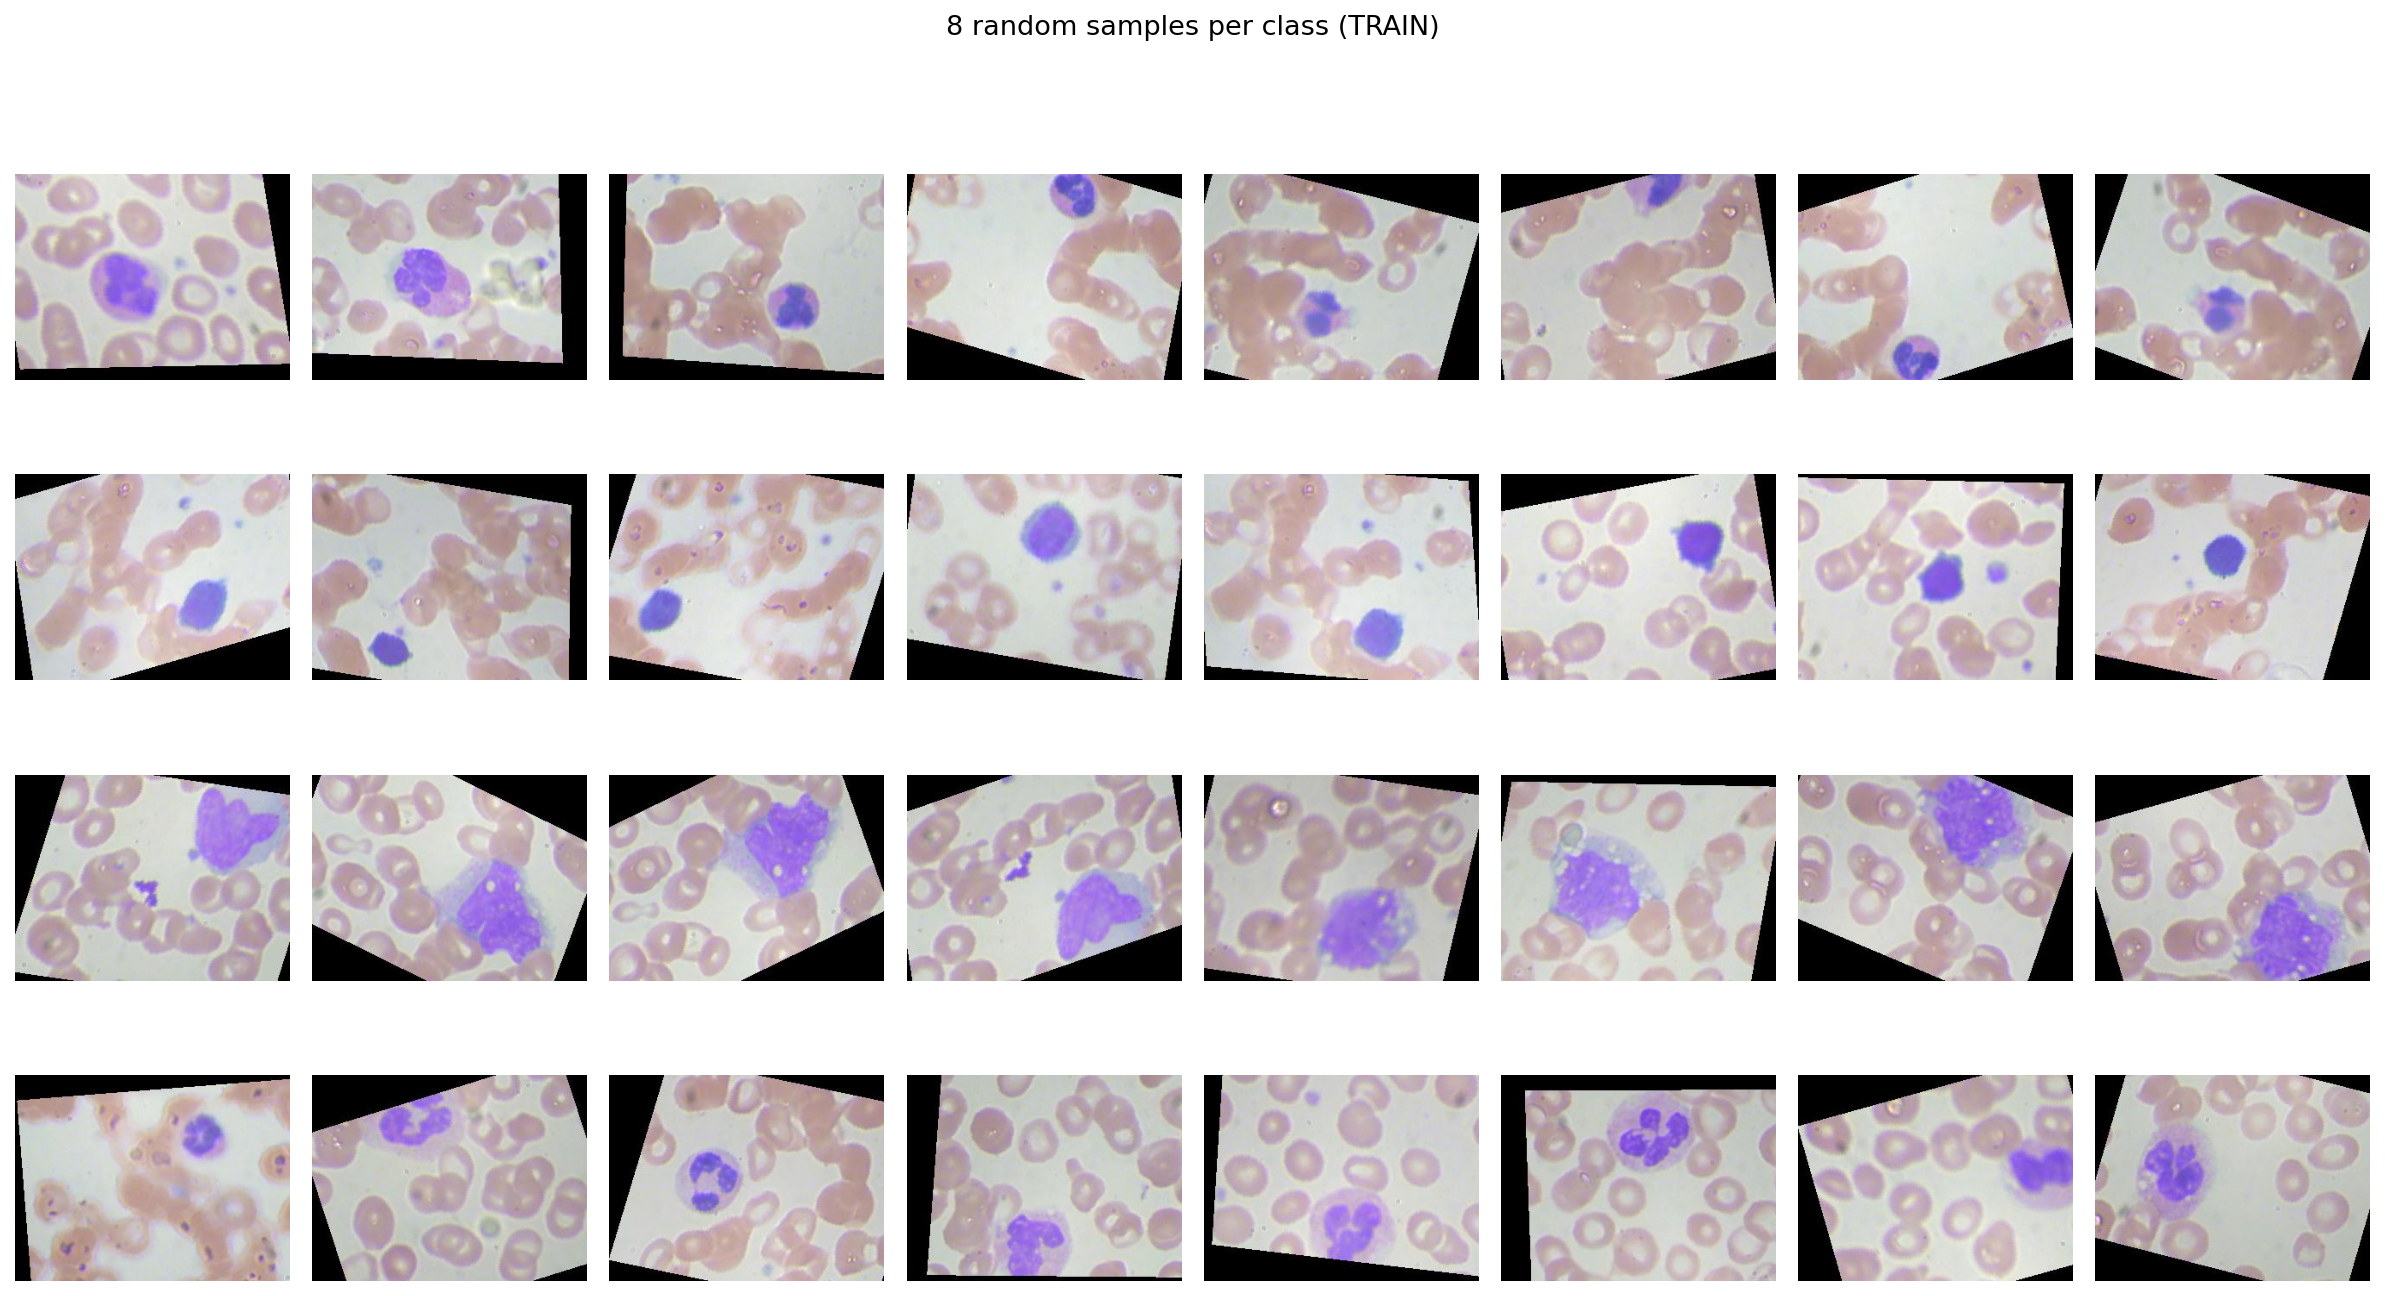
\includegraphics[width=\linewidth]{../outputs/figures/eda_01_sample_grid.png}
    \caption{۸ نمونه تصادفی از هر کلاس در مجموعه آموزشی}
    \label{fig:sample_grid}
\end{figure}

\subsubsection{توزیع کلاس‌ها}

شکل~\ref{fig:class_dist} نشون می‌ده که توزیع کلاس‌ها توی هر سه بخش تقریباً متوازنه — \lr{EOSINOPHIL} با \lr{2{,}497} نمونه، \lr{LYMPHOCYTE} با \lr{2{,}483}، \lr{MONOCYTE} با \lr{2{,}478} و \lr{NEUTROPHIL} با \lr{2{,}499} تا توی مجموعه آموزشی. خوبیش اینه که این تعادل یعنی نه نیازی به \lr{oversampling} داریم، نه نیازی به وزن‌دهی کلاس — مدل از اول با یه دیتای منصفانه سر و کار داره.

\begin{figure}[H]
    \centering
    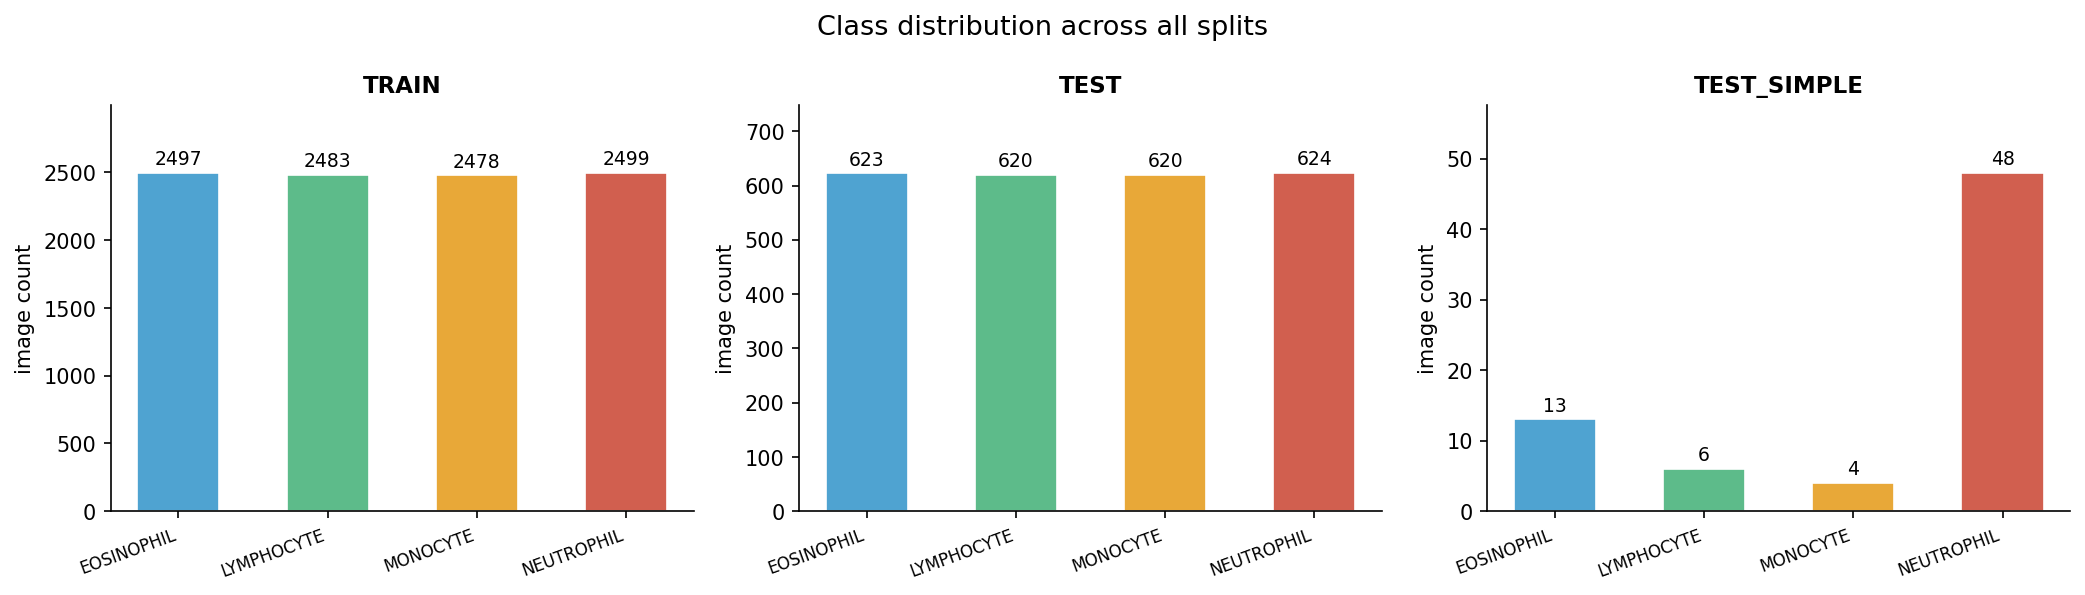
\includegraphics[width=\linewidth]{../outputs/figures/eda_02_class_distribution.png}
    \caption{تعداد تصاویر هر کلاس در سه بخش \lr{TRAIN}، \lr{TEST} و \lr{TEST\_SIMPLE}}
    \label{fig:class_dist}
\end{figure}

\subsubsection{ابعاد تصاویر}

بررسی \lr{300} نمونه تصادفی از مجموعه آموزشی نشون داد که همه تصاویر دقیقاً $320 \times 240$ پیکسل و فرمت \lr{RGB} دارن — هیچ ناهمگونی توی ابعاد نیست. توی مرحله آموزش این تصاویر به $224 \times 224$ پیکسل تغییر اندازه داده می‌شن که هم برای \lr{CNN} سفارشی مناسبه، هم برای \lr{MobileNetV2}.

\subsubsection{توزیع شدت پیکسل}

شکل~\ref{fig:pixel_hist} توزیع سه کانال \lr{R}، \lr{G}، \lr{B} رو برای هر کلاس نشون می‌ده. یه تفاوت جالب اینه که \lr{Eosinophil} بخاطر رنگ‌آمیزی \lr{eosin} یه غلبه قرمز-صورتی مشخص داره، در حالی که \lr{Neutrophil} توزیع آبی بیشتری نشون می‌ده. درنتیجه رنگ به تنهایی می‌تونه یه سیگنال قوی برای تفکیک کلاس‌ها باشه، که این برای مدل یه مزیت حسابه.

\begin{figure}[H]
    \centering
    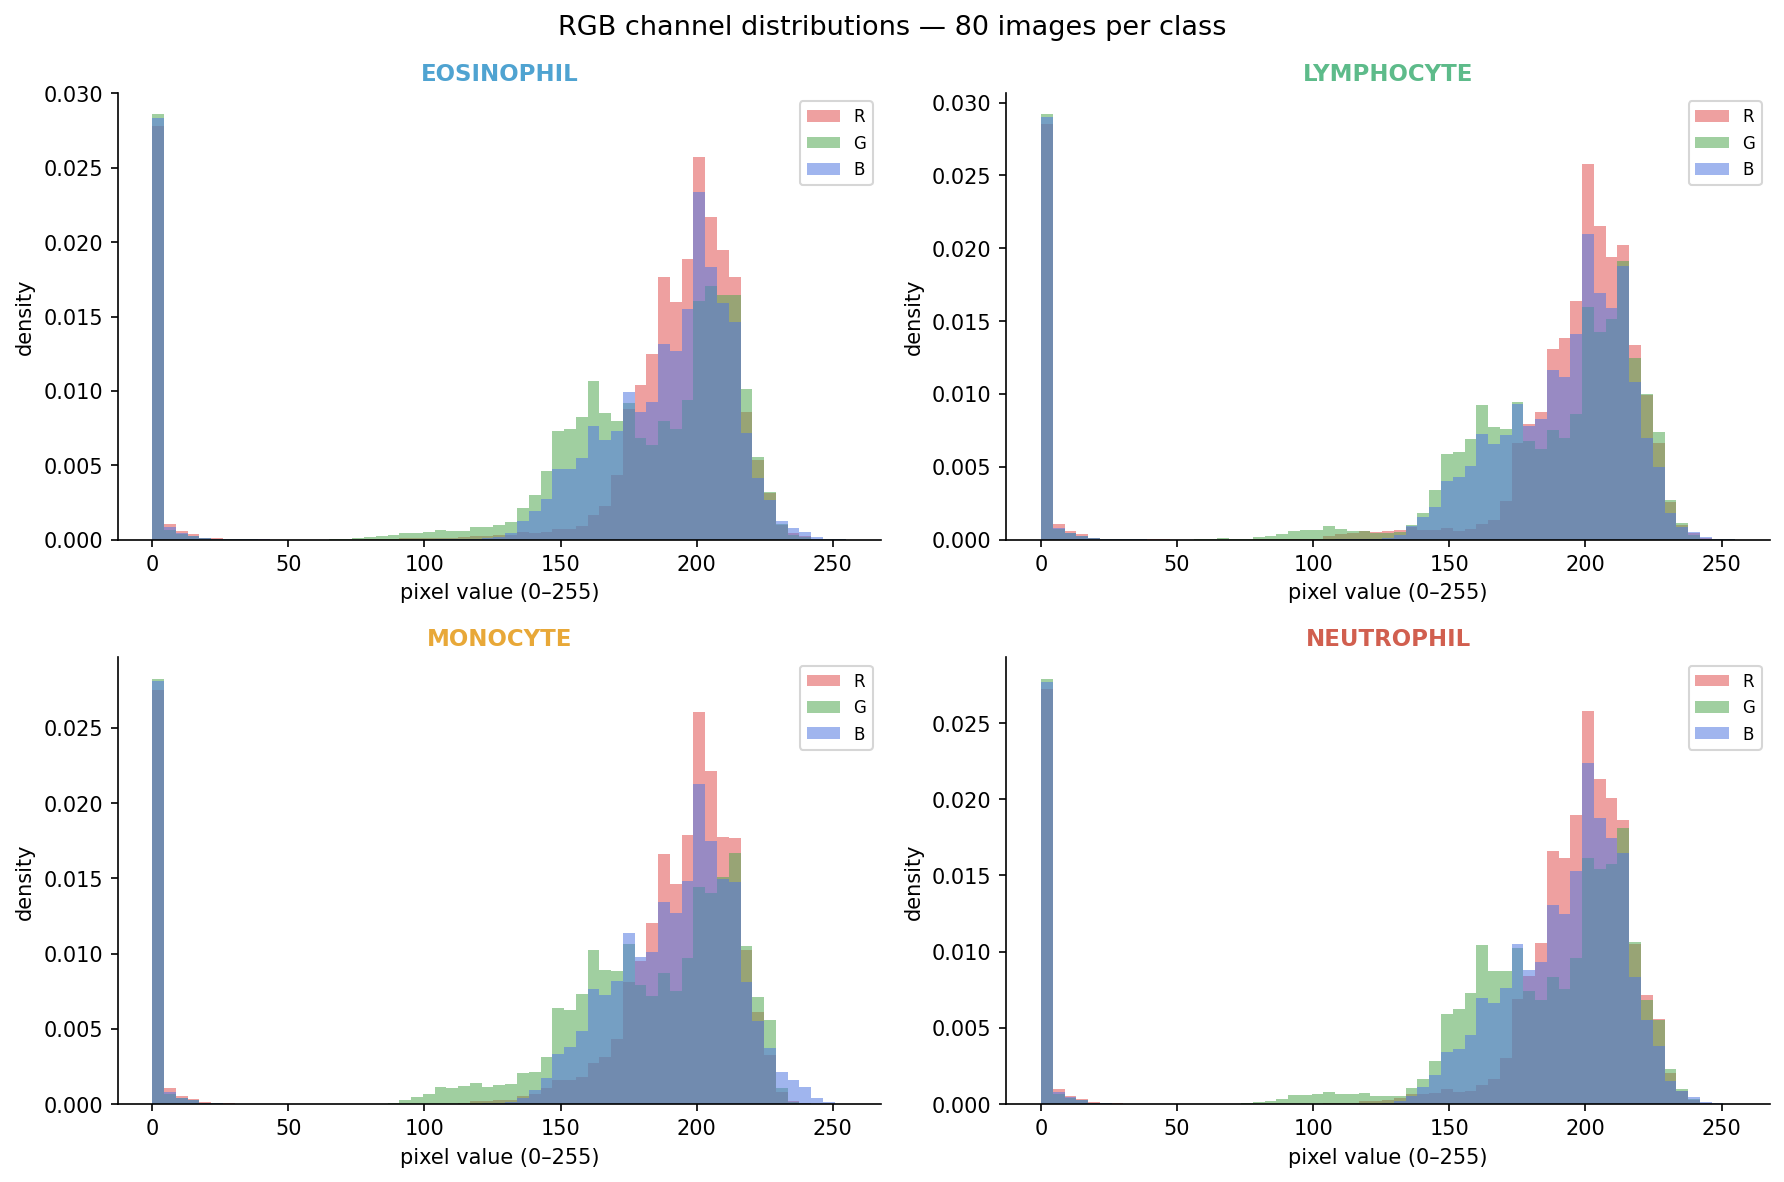
\includegraphics[width=\linewidth]{../outputs/figures/eda_03_pixel_histograms.png}
    \caption{توزیع شدت کانال‌های \lr{RGB} برای ۸۰ نمونه از هر کلاس}
    \label{fig:pixel_hist}
\end{figure}

\subsubsection{تصویر میانگین هر کلاس}

شکل~\ref{fig:mean_img} میانگین \lr{100} تصویر از هر کلاس رو نشون می‌ده. نکته مهم اینه که این تصاویر میانگین هنوزم تیز و قابل تشخیصن — انگار شکل کلی سلول توی همه نمونه‌های یه کلاس خیلی مشابهه. این یعنی هر کلاس از نظر ظاهری نسبتاً همگنه و مدل می‌تونه الگوهای پایدار یاد بگیره.

\begin{figure}[H]
    \centering
    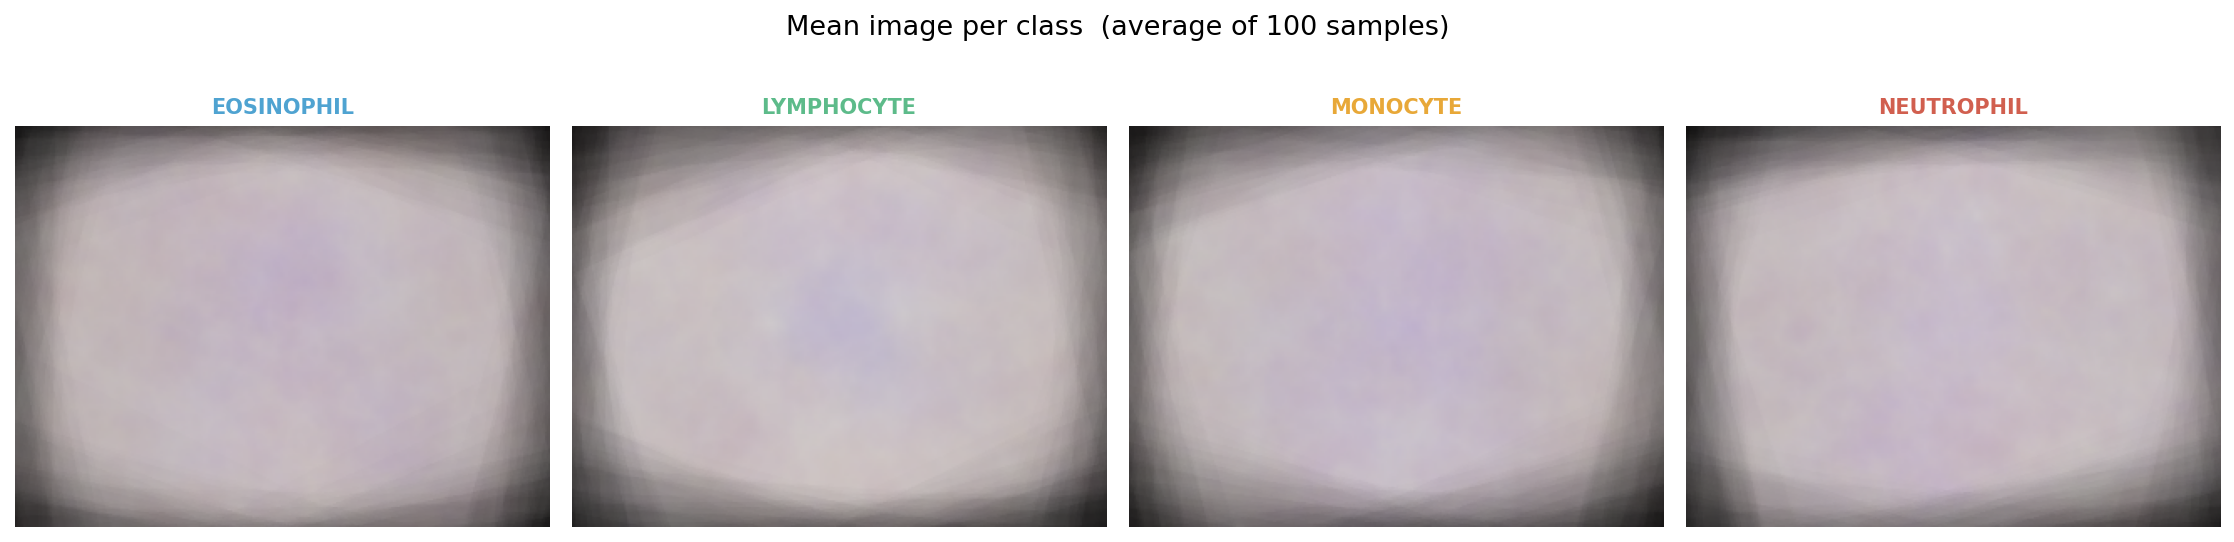
\includegraphics[width=\linewidth]{../outputs/figures/eda_04_mean_images.png}
    \caption{تصویر میانگین هر کلاس (میانگین ۱۰۰ نمونه)}
    \label{fig:mean_img}
\end{figure}

% ---- 3 ----
\section{پیش‌پردازش و افزایش داده}

\subsection{تغییر اندازه و نرمال‌سازی}

همه تصاویر موقع بارگذاری به $224 \times 224$ پیکسل تغییر اندازه داده می‌شن. بعدش مقادیر پیکسل از بازه $[0, 255]$ به $[0, 1]$ نرمال می‌شن:

\[
x_{\text{norm}} = \frac{x}{255}
\]

حالا برای مدل‌های از پیش آموزش‌دیده یه فرق مهم وجود داره — به‌جای این تقسیم ساده، از تابع \lr{preprocess\_input} مخصوص همون مدل استفاده می‌شه که نرمال‌سازی رو متناسب با وزن‌های \lr{ImageNet} اعمال می‌کنه. این یه نکته ظریفه که اگه رعایت نشه، مدل از پیش آموزش‌دیده خوب کار نمی‌کنه. شکل~\ref{fig:preprocess} اثر این پیش‌پردازش رو نشون می‌ده.

\begin{figure}[H]
    \centering
    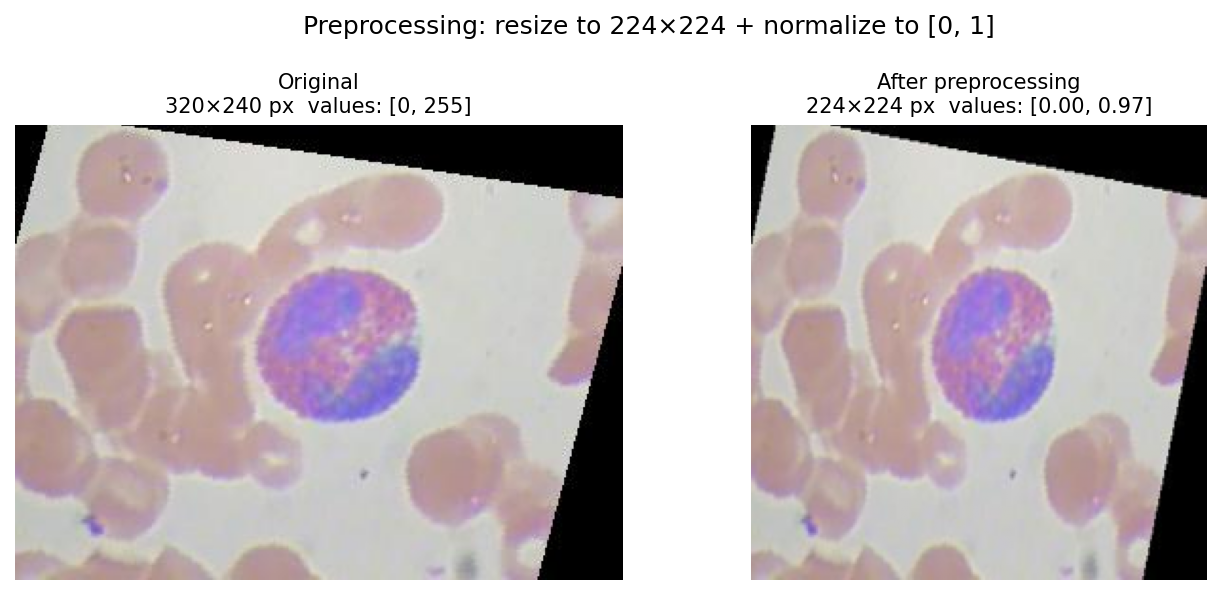
\includegraphics[width=0.75\linewidth]{../outputs/figures/eda_06_preprocessing.png}
    \caption{تصویر اصلی در مقابل تصویر پیش‌پردازش‌شده (تغییر اندازه به $224\times224$ و نرمال‌سازی)}
    \label{fig:preprocess}
\end{figure}

\subsection{تقسیم داده: آموزش و اعتبارسنجی}

بخش \lr{TRAIN} با نسبت \lr{80/20} تقسیم می‌شه — یعنی \lr{7{,}968} تصویر برای آموزش و \lr{1{,}989} تصویر برای اعتبارسنجی. این تقسیم تصادفیه و با \lr{seed=42} انجام می‌شه که نتایج بازتولیدپذیر باشن.

\begin{table}[H]
    \centering
    \begin{tabular}{lccc}
        \toprule
        \textbf{بخش} & \textbf{تعداد تصاویر} & \textbf{درصد} & \textbf{کاربرد} \\
        \midrule
        آموزش (\lr{train})           & \lr{7{,}968} & \lr{80\%} & به‌روزرسانی وزن‌های مدل \\
        اعتبارسنجی (\lr{validation}) & \lr{1{,}989} & \lr{20\%} & انتخاب بهترین \lr{checkpoint} \\
        آزمون (\lr{test})            & \lr{2{,}487} & ---       & ارزیابی نهایی مستقل \\
        \bottomrule
    \end{tabular}
    \caption{تقسیم داده‌ها برای آموزش، اعتبارسنجی و آزمون}
    \label{tab:splits}
\end{table}

\subsection{ساخت \lr{Data Generator}}

برای هر سه بخش یه \lr{generator} جداگانه با \lr{ImageDataGenerator} کرس ساخته می‌شه. \lr{generator} آموزش شامل افزایش داده و \lr{shuffle} هست، ولی \lr{generator}های اعتبارسنجی و آزمون فقط نرمال‌سازی دارن و \lr{shuffle} نمی‌شن.

چرا این تفاوت مهمه؟ خب، توی \lr{train} اگه \lr{shuffle} نباشه ممکنه یه \lr{batch} کامل فقط از یه کلاس بشه که این گرادیان‌های به‌روزرسانی رو بی‌ثبات می‌کنه و آموزش ضعیفی به مدل می‌ده. از طرف دیگه، \lr{validation} و \lr{test} نباید \lr{shuffle} بشن چون می‌خوایم نتایج ارزیابی هر بار دقیقاً یکسون باشن و بشه پیش‌بینی‌ها رو دقیقاً به تصاویر متناظرشون نسبت داد. درنتیجه این دو تا تنظیم مکمل همن، نه اشتباه.

\subsection{افزایش داده}

افزایش داده (\lr{Data Augmentation}) فقط روی مجموعه آموزشی اعمال می‌شه — این یه نکته اساسیه که نباید فراموش بشه. هر تبدیلی که انتخاب شده یه دلیل فیزیکی داره که از ماهیت تصاویر میکروسکوپی میاد:

\begin{table}[H]
    \centering
    \begin{tabular}{lll}
        \toprule
        \textbf{تبدیل} & \textbf{مقدار} & \textbf{دلیل} \\
        \midrule
        چرخش & $\pm 15°$ & سلول‌ها در تمام جهات ظاهر می‌شوند \\
        انعکاس افقی & فعال & تصویر آینه‌ای در میکروسکوپ معتبر است \\
        انعکاس عمودی & فعال & جهت بالا/پایین در میکروسکوپ اهمیتی ندارد \\
        جابجایی افقی/عمودی & $\pm 10\%$ & سلول همیشه دقیقاً در مرکز نیست \\
        زوم & $\pm 10\%$ & تغییر بزرگنمایی میکروسکوپ \\
        روشنایی & $\pm 20\%$ & شدت رنگ‌آمیزی بین اسلایدها متفاوت است \\
        حالت پر کردن & \lr{nearest} & از ایجاد لبه‌های سیاه جلوگیری می‌کند \\
        \bottomrule
    \end{tabular}
    \caption{تبدیل‌های افزایش داده و توجیه آن‌ها}
    \label{tab:augmentation}
\end{table}

اینجوریه که مدل یاد می‌گیره به تغییرات غیرمعنادار حساس نباشه — انگار که هر بار یه نمونه جدید می‌بینه، در حالی که دیتاست اصلی همونه. شکل~\ref{fig:augmentation} نمونه‌ای از تصویر اصلی در کنار ۶ نسخه افزوده‌شده رو برای هر کلاس نشون می‌ده.

\begin{figure}[H]
    \centering
    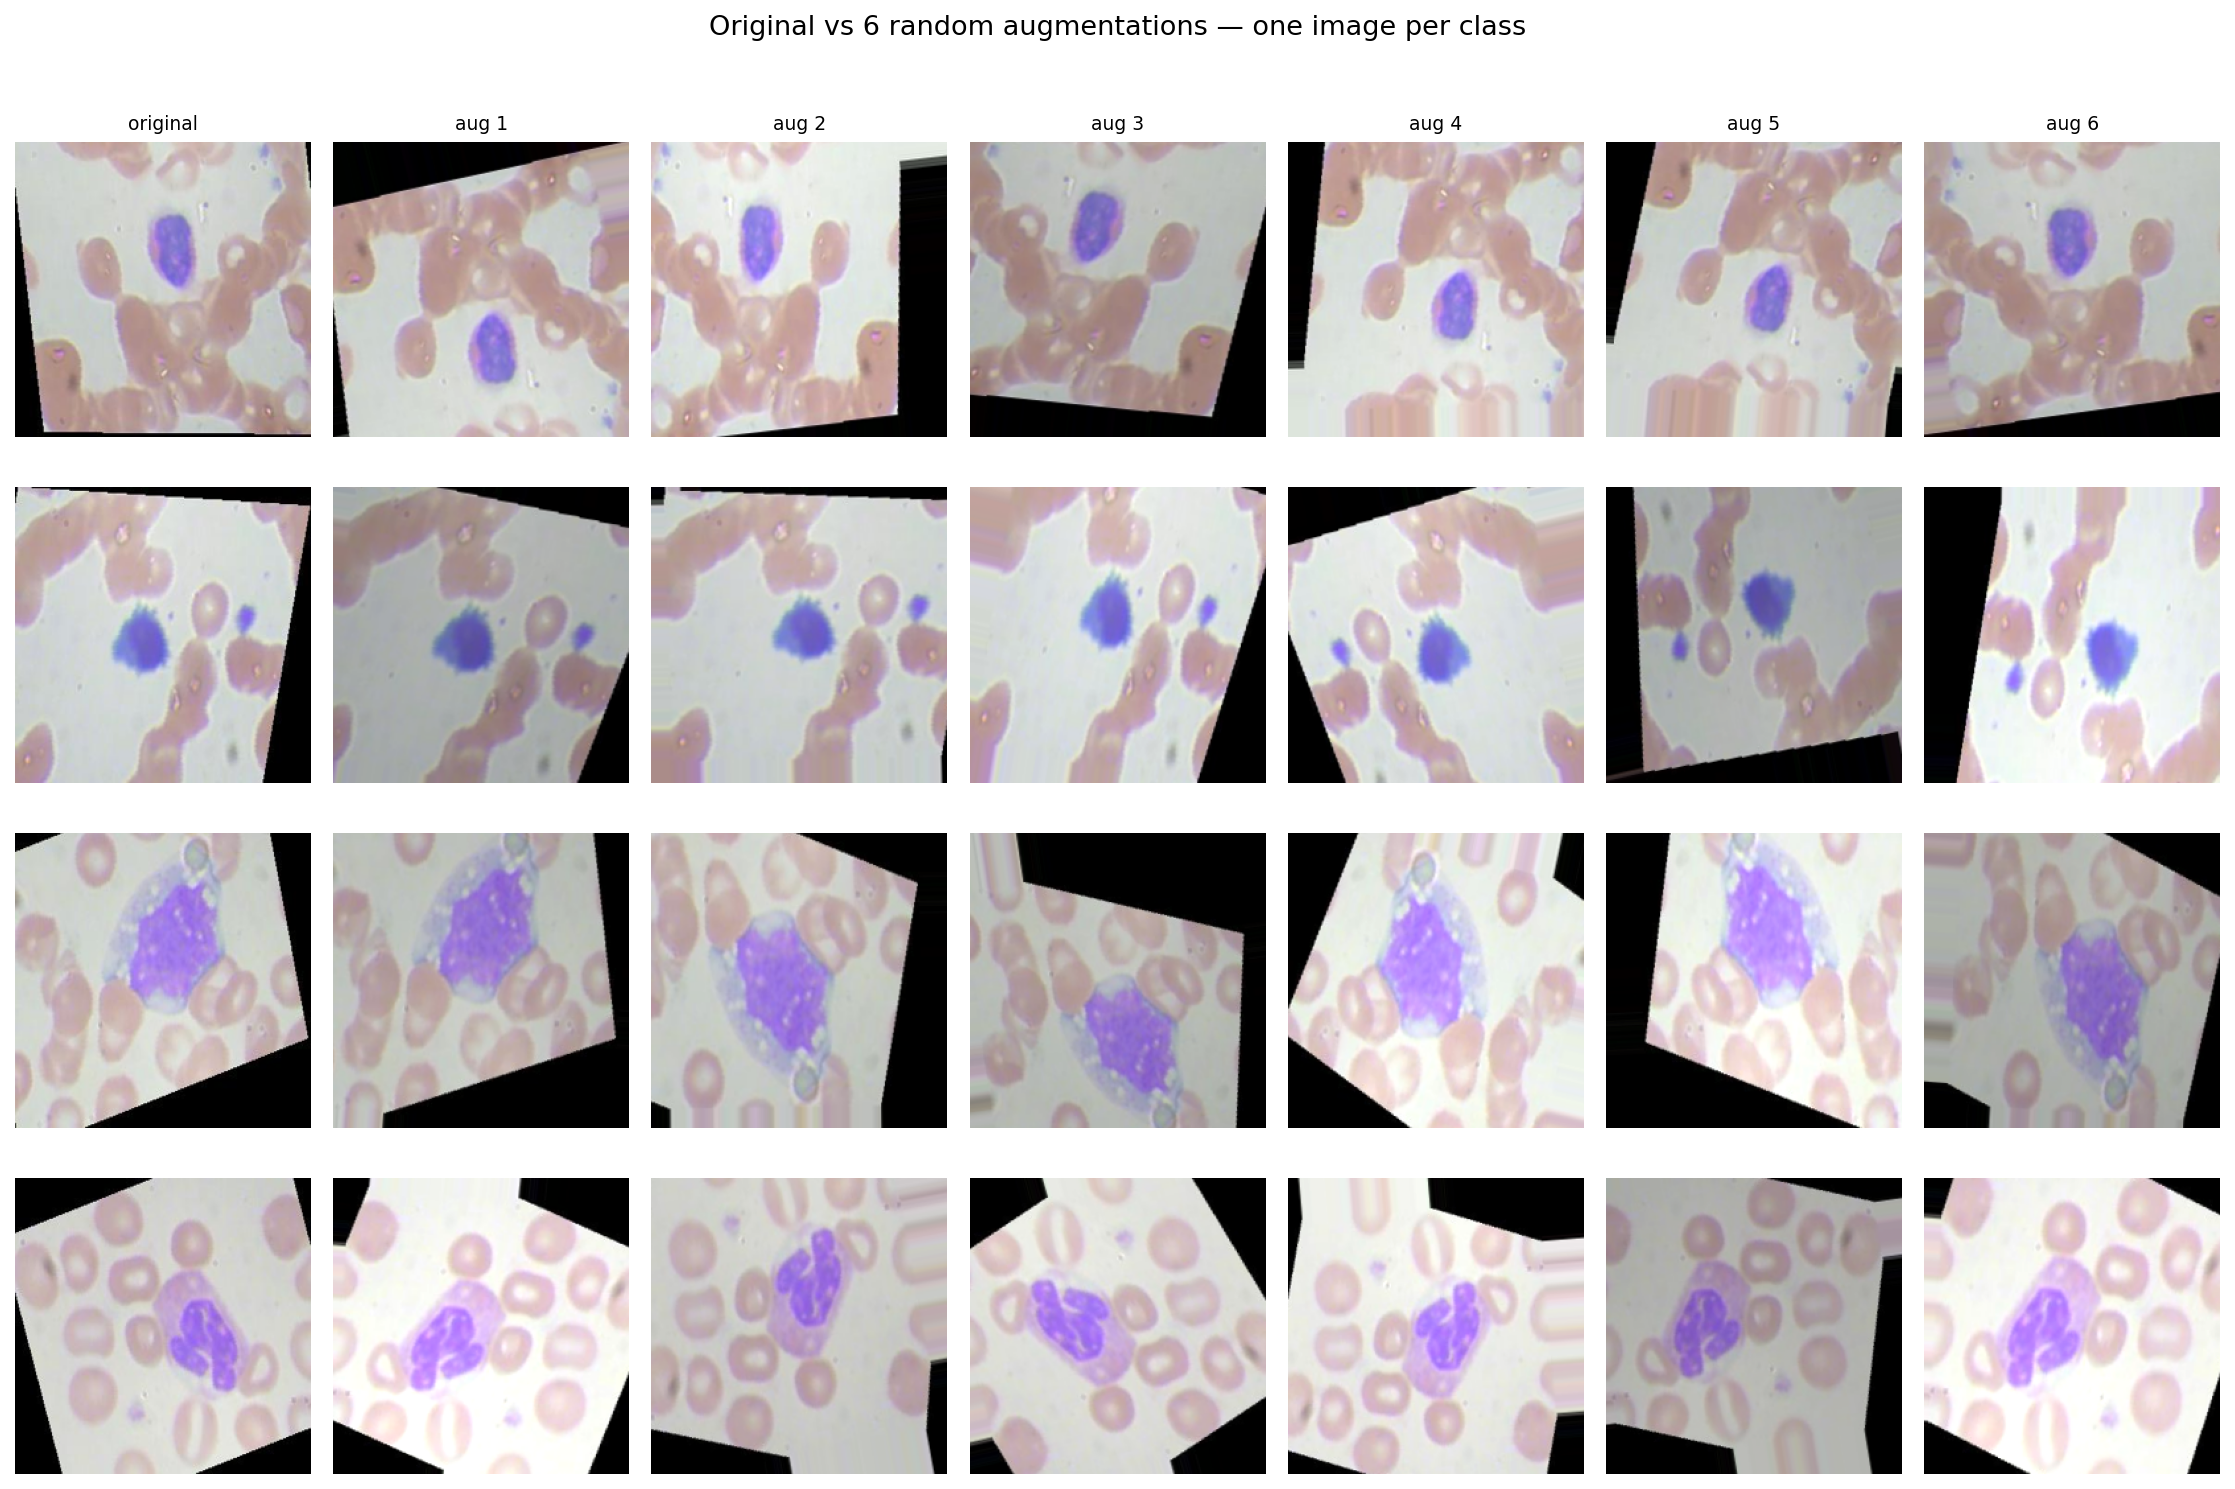
\includegraphics[width=\linewidth]{../outputs/figures/eda_05_augmentation_preview.png}
    \caption{تصویر اصلی در مقابل ۶ نسخه افزوده‌شده برای یک نمونه از هر کلاس}
    \label{fig:augmentation}
\end{figure}

\subsection{نمایش یک \lr{batch} از داده‌های آموزشی}

شکل~\ref{fig:batch} یه \lr{batch} نمونه از \lr{generator} آموزشی رو نشون می‌ده. هر \lr{batch} شامل ۳۲ تصویر با شکل $(32, 224, 224, 3)$ و برچسب‌های \lr{one-hot} با شکل $(32, 4)$ هست — پس ورودی و خروجی مدل دقیقاً همین ابعادن.

\begin{figure}[H]
    \centering
    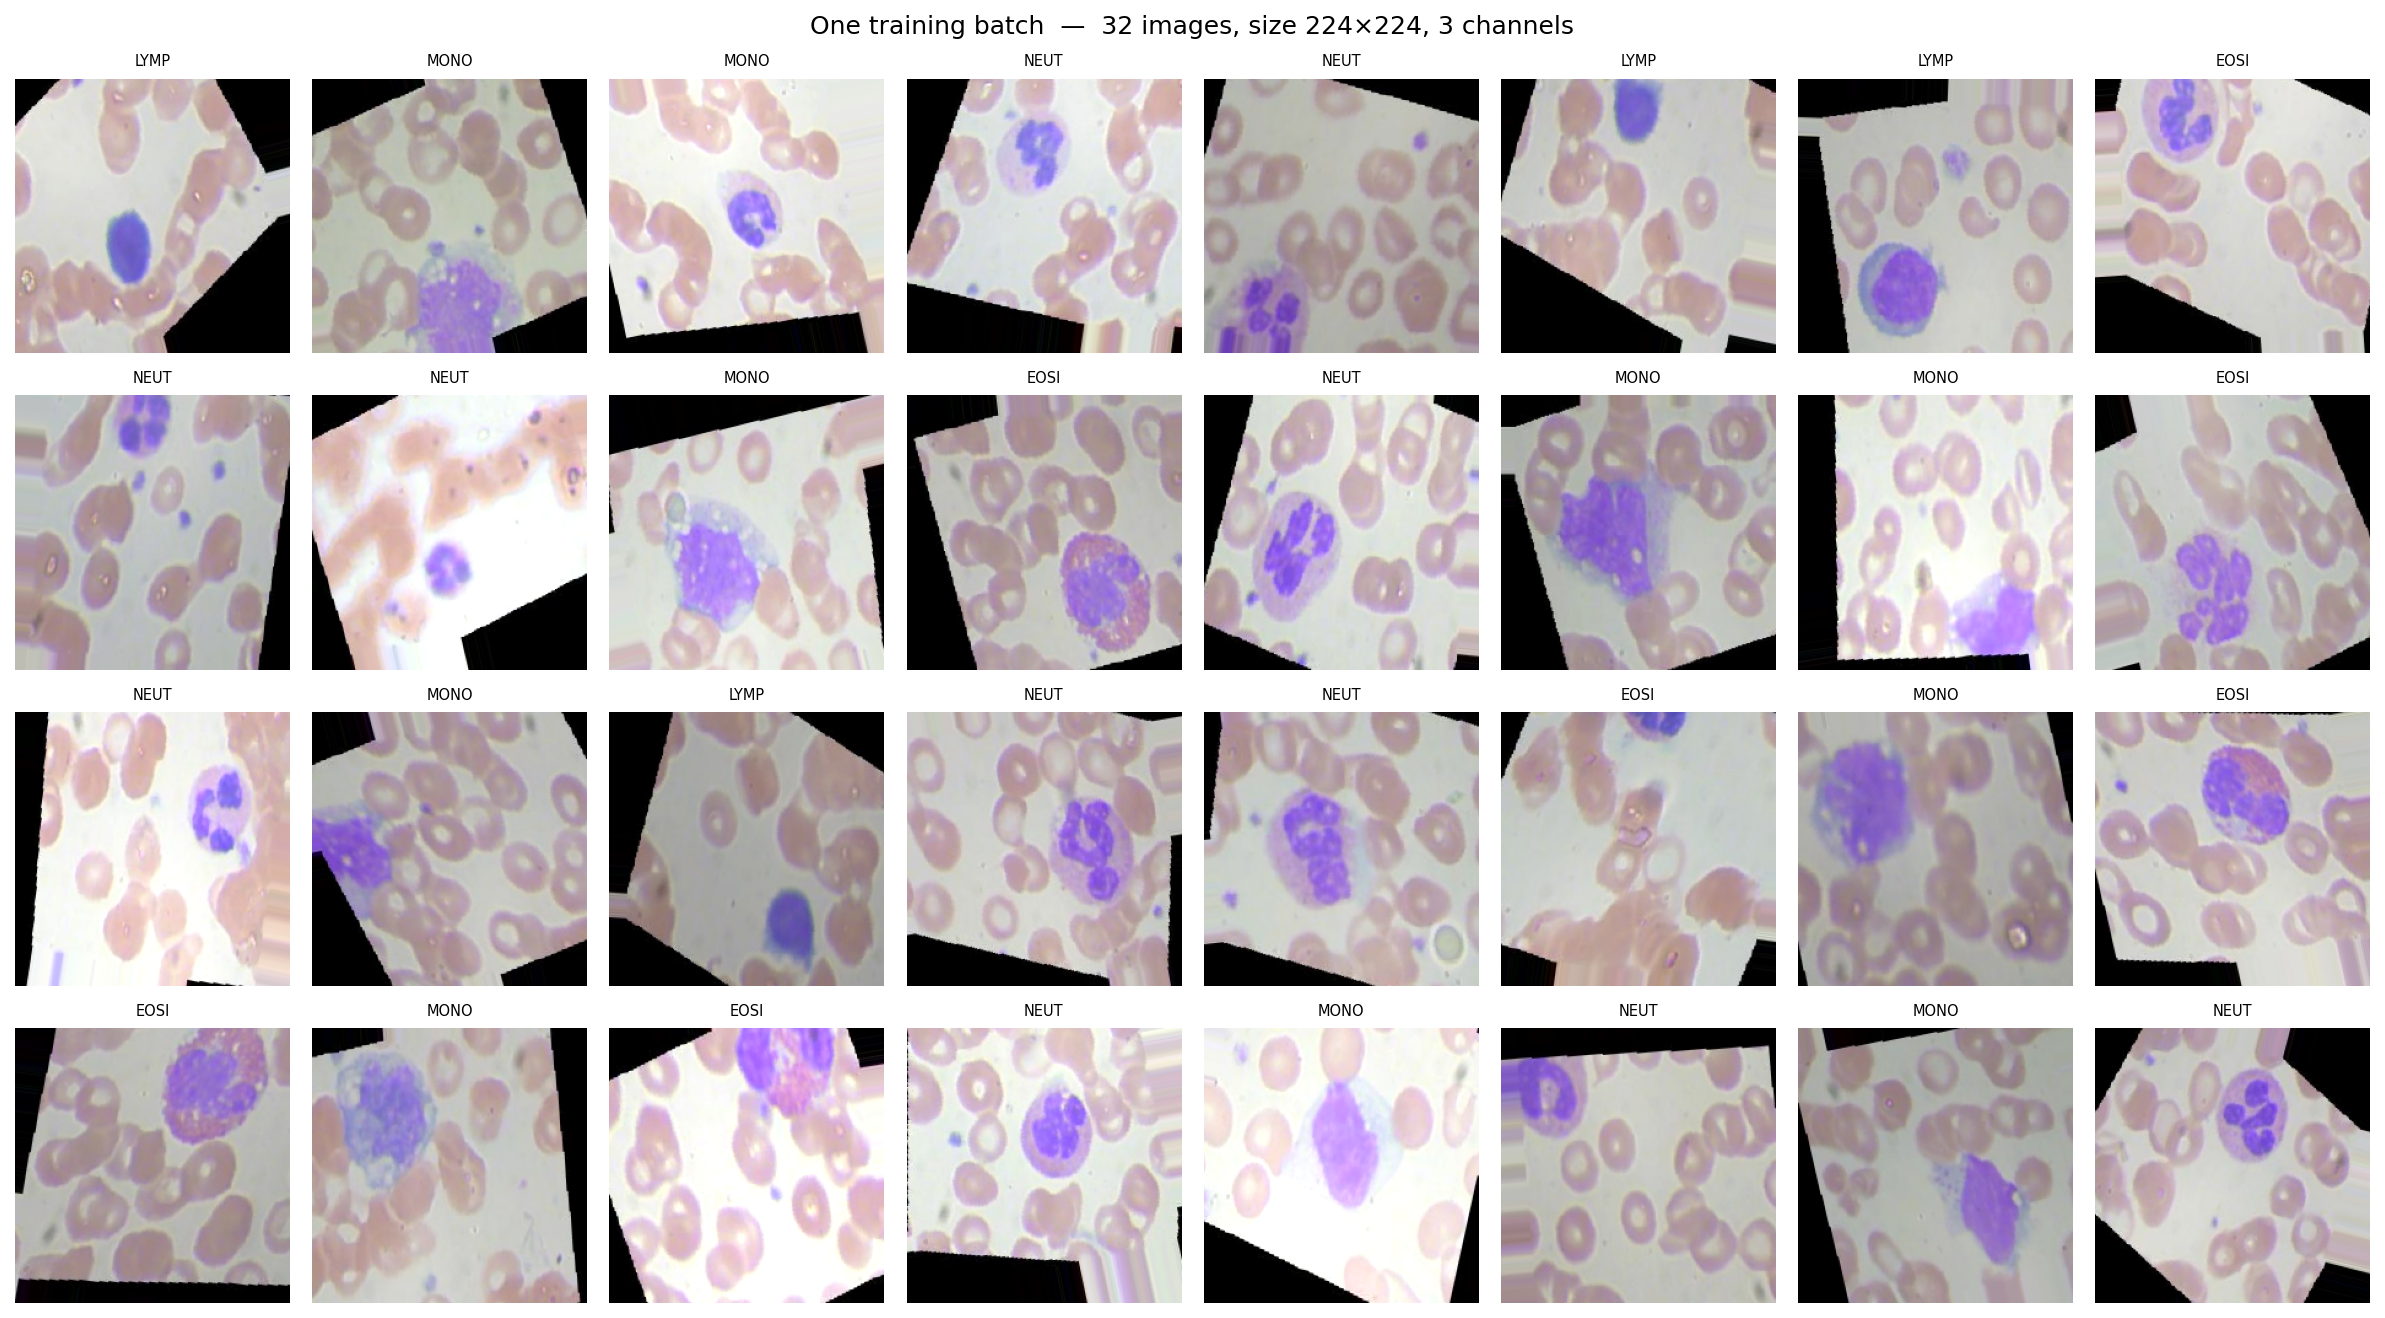
\includegraphics[width=\linewidth]{../outputs/figures/eda_07_batch_display.png}
    \caption{یک \lr{batch} از داده‌های آموزشی — ۳۲ تصویر $224\times224$ با برچسب کلاس}
    \label{fig:batch}
\end{figure}

% ---- 4 ----
\section{مدل \lr{CNN} از پایه}

\subsection{معماری}

خب، اولین کاری که کردیم اینه که یه \lr{CNN} ساده از صفر نوشتیم — بدون وزن از پیش آموزش‌دیده، بدون \lr{Dropout}، بدون \lr{BatchNorm}، بدون هیچ افزایش داده‌ای. هدف اینه که یه \lr{baseline} داشته باشیم که بفهمیم فازهای بعدی چقدر بهترش کردن.

معماری شبکه چهار بلوک کانولوشنی داره که هر کدوم از یه \lr{Conv2D} با \lr{ReLU} و یه \lr{MaxPooling} تشکیل شدن. بعد از این چهار بلوک، یه \lr{Flatten} داریم و دو لایه‌ی \lr{Dense} — اولی با \lr{ReLU} و دومی با \lr{Softmax} که چهار کلاس خروجی میده:

\[
\text{ورودی}\ (128 \times 128 \times 3)
\;\xrightarrow{\text{Conv32+Pool}}\;
\xrightarrow{\text{Conv64+Pool}}\;
\xrightarrow{\text{Conv128+Pool}}\;
\xrightarrow{\text{Conv128+Pool}}\;
\xrightarrow{\text{Flatten}}\;
\xrightarrow{\text{Dense64}}\;
\xrightarrow{\text{Dense4}}
\]

\begin{table}[H]
    \centering
    \begin{tabular}{llcr}
        \toprule
        \textbf{لایه} & \textbf{نوع} & \textbf{شکل خروجی} & \textbf{تعداد پارامتر} \\
        \midrule
        ورودی            & \lr{Input}       & $128 \times 128 \times 3$  & --- \\
        بلوک ۱           & \lr{Conv2D(32)}  & $128 \times 128 \times 32$ & \lr{896} \\
                         & \lr{MaxPool}     & $64 \times 64 \times 32$   & --- \\
        بلوک ۲           & \lr{Conv2D(64)}  & $64 \times 64 \times 64$   & \lr{18{,}496} \\
                         & \lr{MaxPool}     & $32 \times 32 \times 64$   & --- \\
        بلوک ۳           & \lr{Conv2D(128)} & $32 \times 32 \times 128$  & \lr{73{,}856} \\
                         & \lr{MaxPool}     & $16 \times 16 \times 128$  & --- \\
        بلوک ۴           & \lr{Conv2D(128)} & $16 \times 16 \times 128$  & \lr{147{,}584} \\
                         & \lr{MaxPool}     & $8 \times 8 \times 128$    & --- \\
        \lr{Flatten}     & ---              & $8192$                     & --- \\
        \lr{Dense(64)}   & \lr{ReLU}        & $64$                       & \lr{524{,}352} \\
        \lr{Dense(4)}    & \lr{Softmax}     & $4$                        & \lr{260} \\
        \midrule
        \textbf{جمع پارامترها} & & & \textbf{\lr{765{,}444}} \\
        \bottomrule
    \end{tabular}
    \caption{معماری \lr{Baseline CNN} — کمتر از یک میلیون پارامتر}
    \label{tab:baseline_arch}
\end{table}

درواقع کل شبکه \lr{765{,}444} پارامتر قابل آموزش داره که خوشبختانه زیر سقف یک میلیون پارامتر می‌مونه.

\subsection{تنظیمات آموزش}

\begin{table}[H]
    \centering
    \begin{tabular}{ll}
        \toprule
        \textbf{تنظیم} & \textbf{مقدار} \\
        \midrule
        بهینه‌ساز         & \lr{Adam} \\
        نرخ یادگیری      & $0.0001$ \\
        تابع هزینه        & \lr{Categorical Cross-Entropy} \\
        اندازه \lr{batch} & $32$ \\
        تعداد \lr{epoch}  & $30$ \\
        اندازه تصویر      & $128 \times 128$ پیکسل \\
        نرمال‌سازی        & تقسیم بر $255$ \\
        ذخیره بهترین مدل  & \lr{ModelCheckpoint} بر اساس \lr{val\_accuracy} \\
        \bottomrule
    \end{tabular}
    \caption{تنظیمات آموزش \lr{Baseline CNN}}
    \label{tab:baseline_train}
\end{table}

\subsection{نمودار آموزش}

شکل~\ref{fig:baseline_curves} روند \lr{loss} و دقت رو در طول \lr{30} \lr{epoch} برای هر دو مجموعه‌ی آموزش و اعتبارسنجی نشون می‌ده.

\begin{figure}[H]
    \centering
    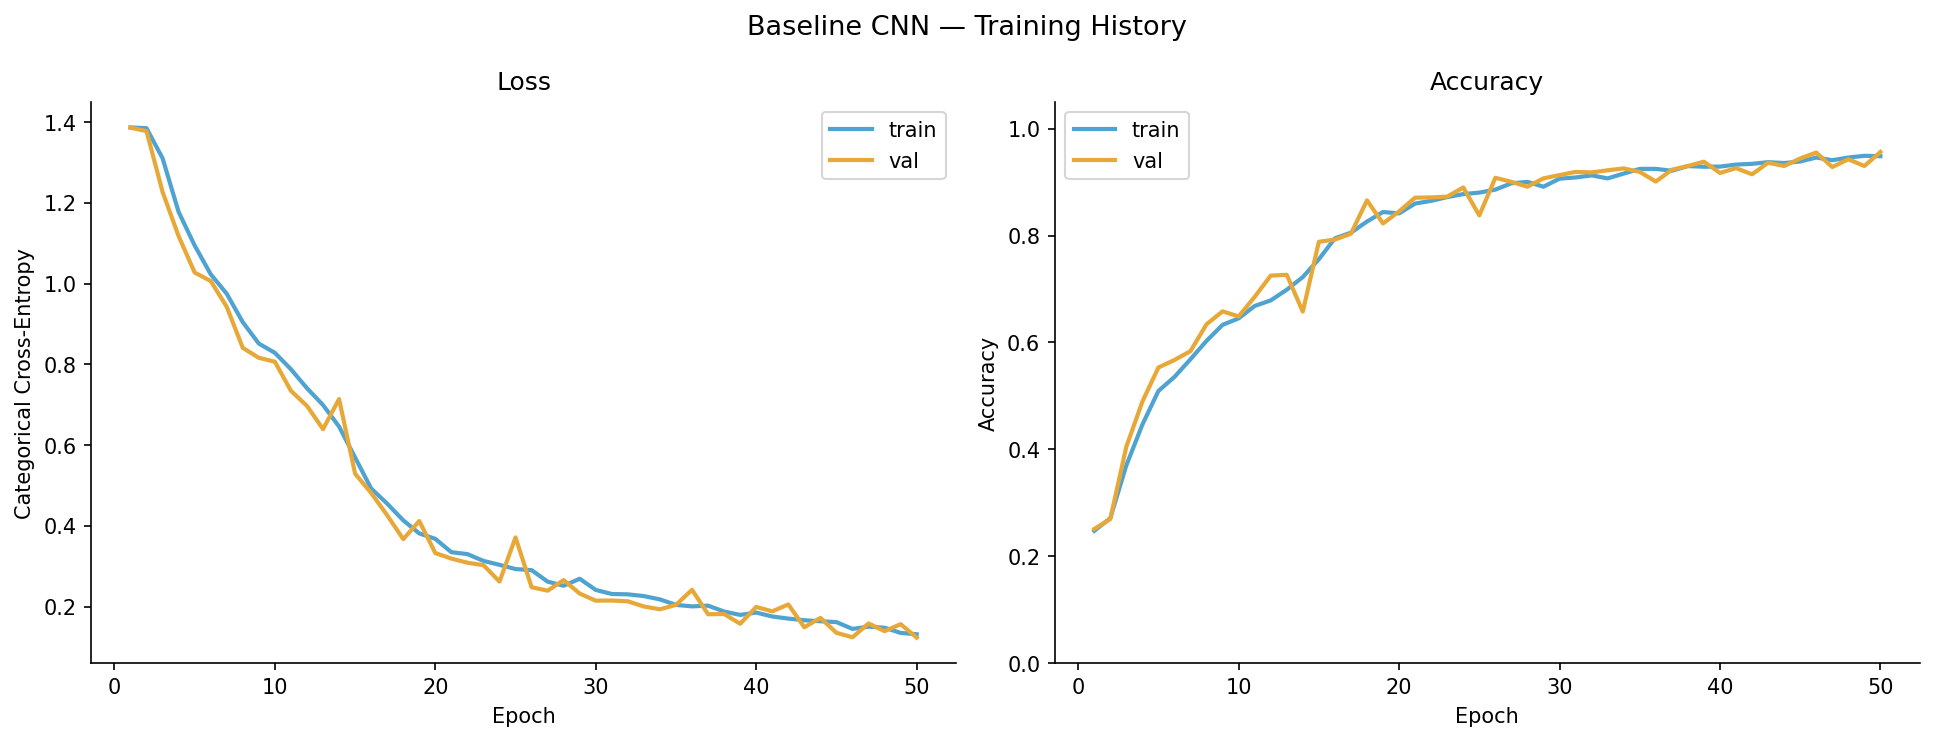
\includegraphics[width=\linewidth]{../outputs/figures/phase2_01_training_curves.png}
    \caption{نمودار \lr{loss} و دقت در طول آموزش — \lr{Baseline CNN}}
    \label{fig:baseline_curves}
\end{figure}

چیزی که توی این نمودار جالبه اینه که هر دو منحنی آموزش و اعتبارسنجی کاملاً با هم پیش رفتن و تا \lr{epoch} آخر هم \lr{val accuracy} داشت بهتر می‌شد — یعنی مدل هنوز داشت یاد می‌گرفت. دقت آموزشی در پایان به \lr{97.55\%} رسید و دقت اعتبارسنجی به \lr{94.57\%}، که اختلافشون فقط \lr{2.98\%} هست. پس \lr{overfitting} شدیدی اتفاق نیفتاده.

\subsection{ارزیابی روی مجموعه آزمون}

بهترین مدل ذخیره‌شده — که بر اساس \lr{val\_accuracy} انتخاب شده — روی مجموعه‌ی آزمون مستقل ارزیابی شد:

\begin{table}[H]
    \centering
    \begin{tabular}{lc}
        \toprule
        \textbf{معیار} & \textbf{مقدار} \\
        \midrule
        دقت (\lr{Accuracy})           & \lr{79.53\%} \\
        دقت ماکرو (\lr{Precision})    & \lr{81.78\%} \\
        فراخوانی ماکرو (\lr{Recall})  & \lr{79.55\%} \\
        \lr{F1-score} ماکرو           & \lr{80.19\%} \\
        \lr{AUC} ماکرو                & \lr{95.52\%} \\
        \bottomrule
    \end{tabular}
    \caption{نتایج ارزیابی \lr{Baseline CNN} روی مجموعه آزمون}
    \label{tab:baseline_test}
\end{table}

عملکرد مدل به تفکیک هر کلاس در جدول زیر آمده:

\begin{table}[H]
    \centering
    \begin{tabular}{lcccc}
        \toprule
        \textbf{کلاس} & \textbf{\lr{Precision}} & \textbf{\lr{Recall}} & \textbf{\lr{F1}} & \textbf{\lr{AUC}} \\
        \midrule
        \lr{Eosinophil} & \lr{0.65} & \lr{0.73} & \lr{0.69} & \lr{0.9150} \\
        \lr{Lymphocyte} & \lr{1.00} & \lr{0.93} & \lr{0.96} & \lr{0.9996} \\
        \lr{Monocyte}   & \lr{0.97} & \lr{0.76} & \lr{0.85} & \lr{0.9848} \\
        \lr{Neutrophil} & \lr{0.66} & \lr{0.76} & \lr{0.71} & \lr{0.9215} \\
        \bottomrule
    \end{tabular}
    \caption{عملکرد به تفکیک کلاس — \lr{Baseline CNN}}
    \label{tab:baseline_perclass}
\end{table}

\subsection{ماتریس درهم‌ریختگی}

شکل~\ref{fig:baseline_cm} ماتریس درهم‌ریختگی مدل روی مجموعه آزمون را نشان می‌دهد.

\begin{figure}[H]
    \centering
    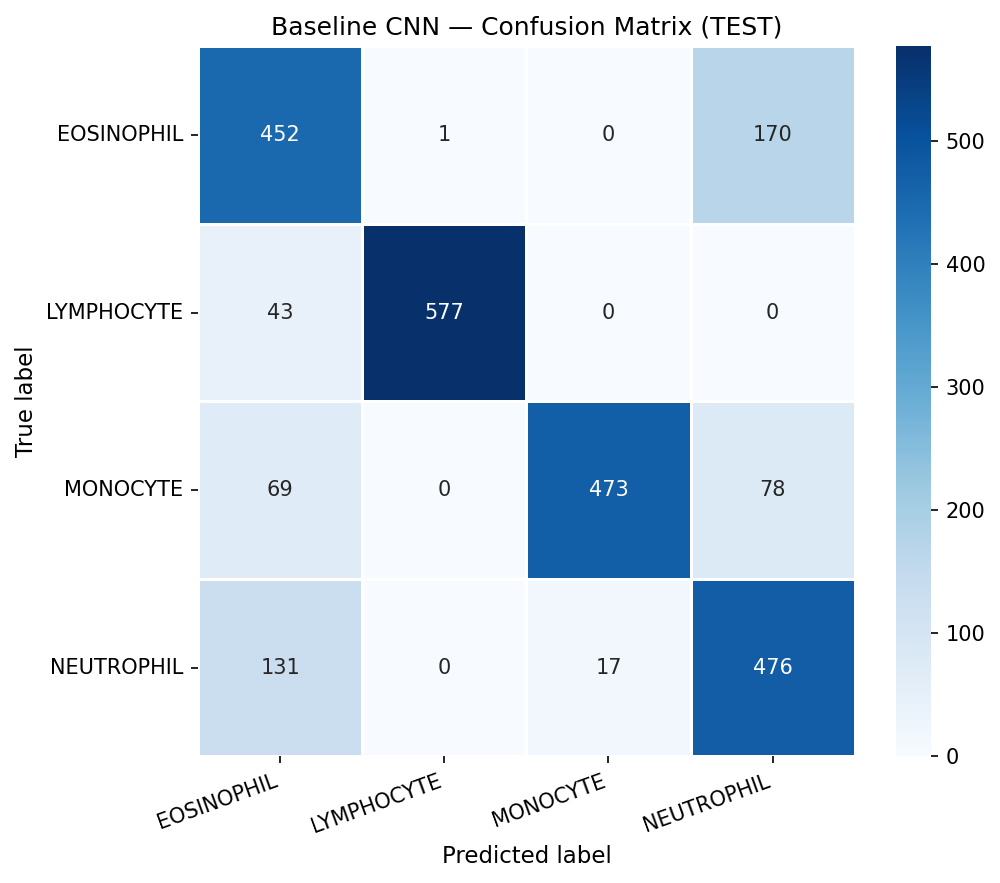
\includegraphics[width=0.72\linewidth]{../outputs/figures/phase2_02_confusion_matrix.png}
    \caption{ماتریس درهم‌ریختگی \lr{Baseline CNN} روی مجموعه آزمون}
    \label{fig:baseline_cm}
\end{figure}

\subsection{منحنی \lr{ROC}}

شکل~\ref{fig:baseline_roc} منحنی‌های \lr{ROC} به تفکیک هر کلاس رو نشون می‌ده. \lr{AUC} مربوط به \lr{Lymphocyte} تقریباً \lr{1.00} هست که انگار مدل این کلاس رو با چشم‌بسته هم می‌شناسه — جداسازیش از بقیه کلاس‌ها کاملاً قطعیه.

\begin{figure}[H]
    \centering
    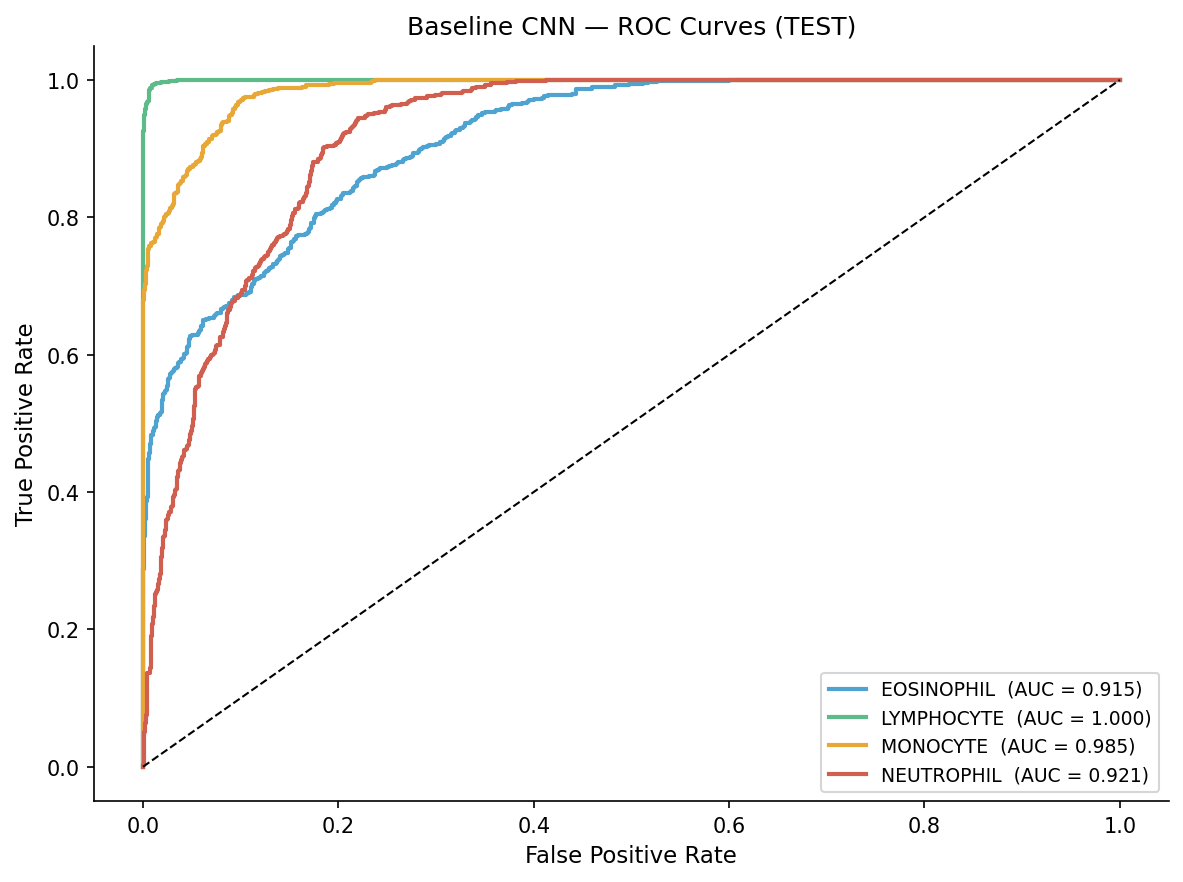
\includegraphics[width=0.7\linewidth]{../outputs/figures/phase2_03_roc_curves.png}
    \caption{منحنی \lr{ROC} برای چهار کلاس — \lr{Baseline CNN}}
    \label{fig:baseline_roc}
\end{figure}

\subsection{نمونه پیش‌بینی‌ها}

شکل~\ref{fig:baseline_preds} چند نمونه از پیش‌بینی‌های مدل رو نشون می‌ده. عنوان سبز یعنی پیش‌بینی درست بوده، قرمز یعنی اشتباه.

\begin{figure}[H]
    \centering
    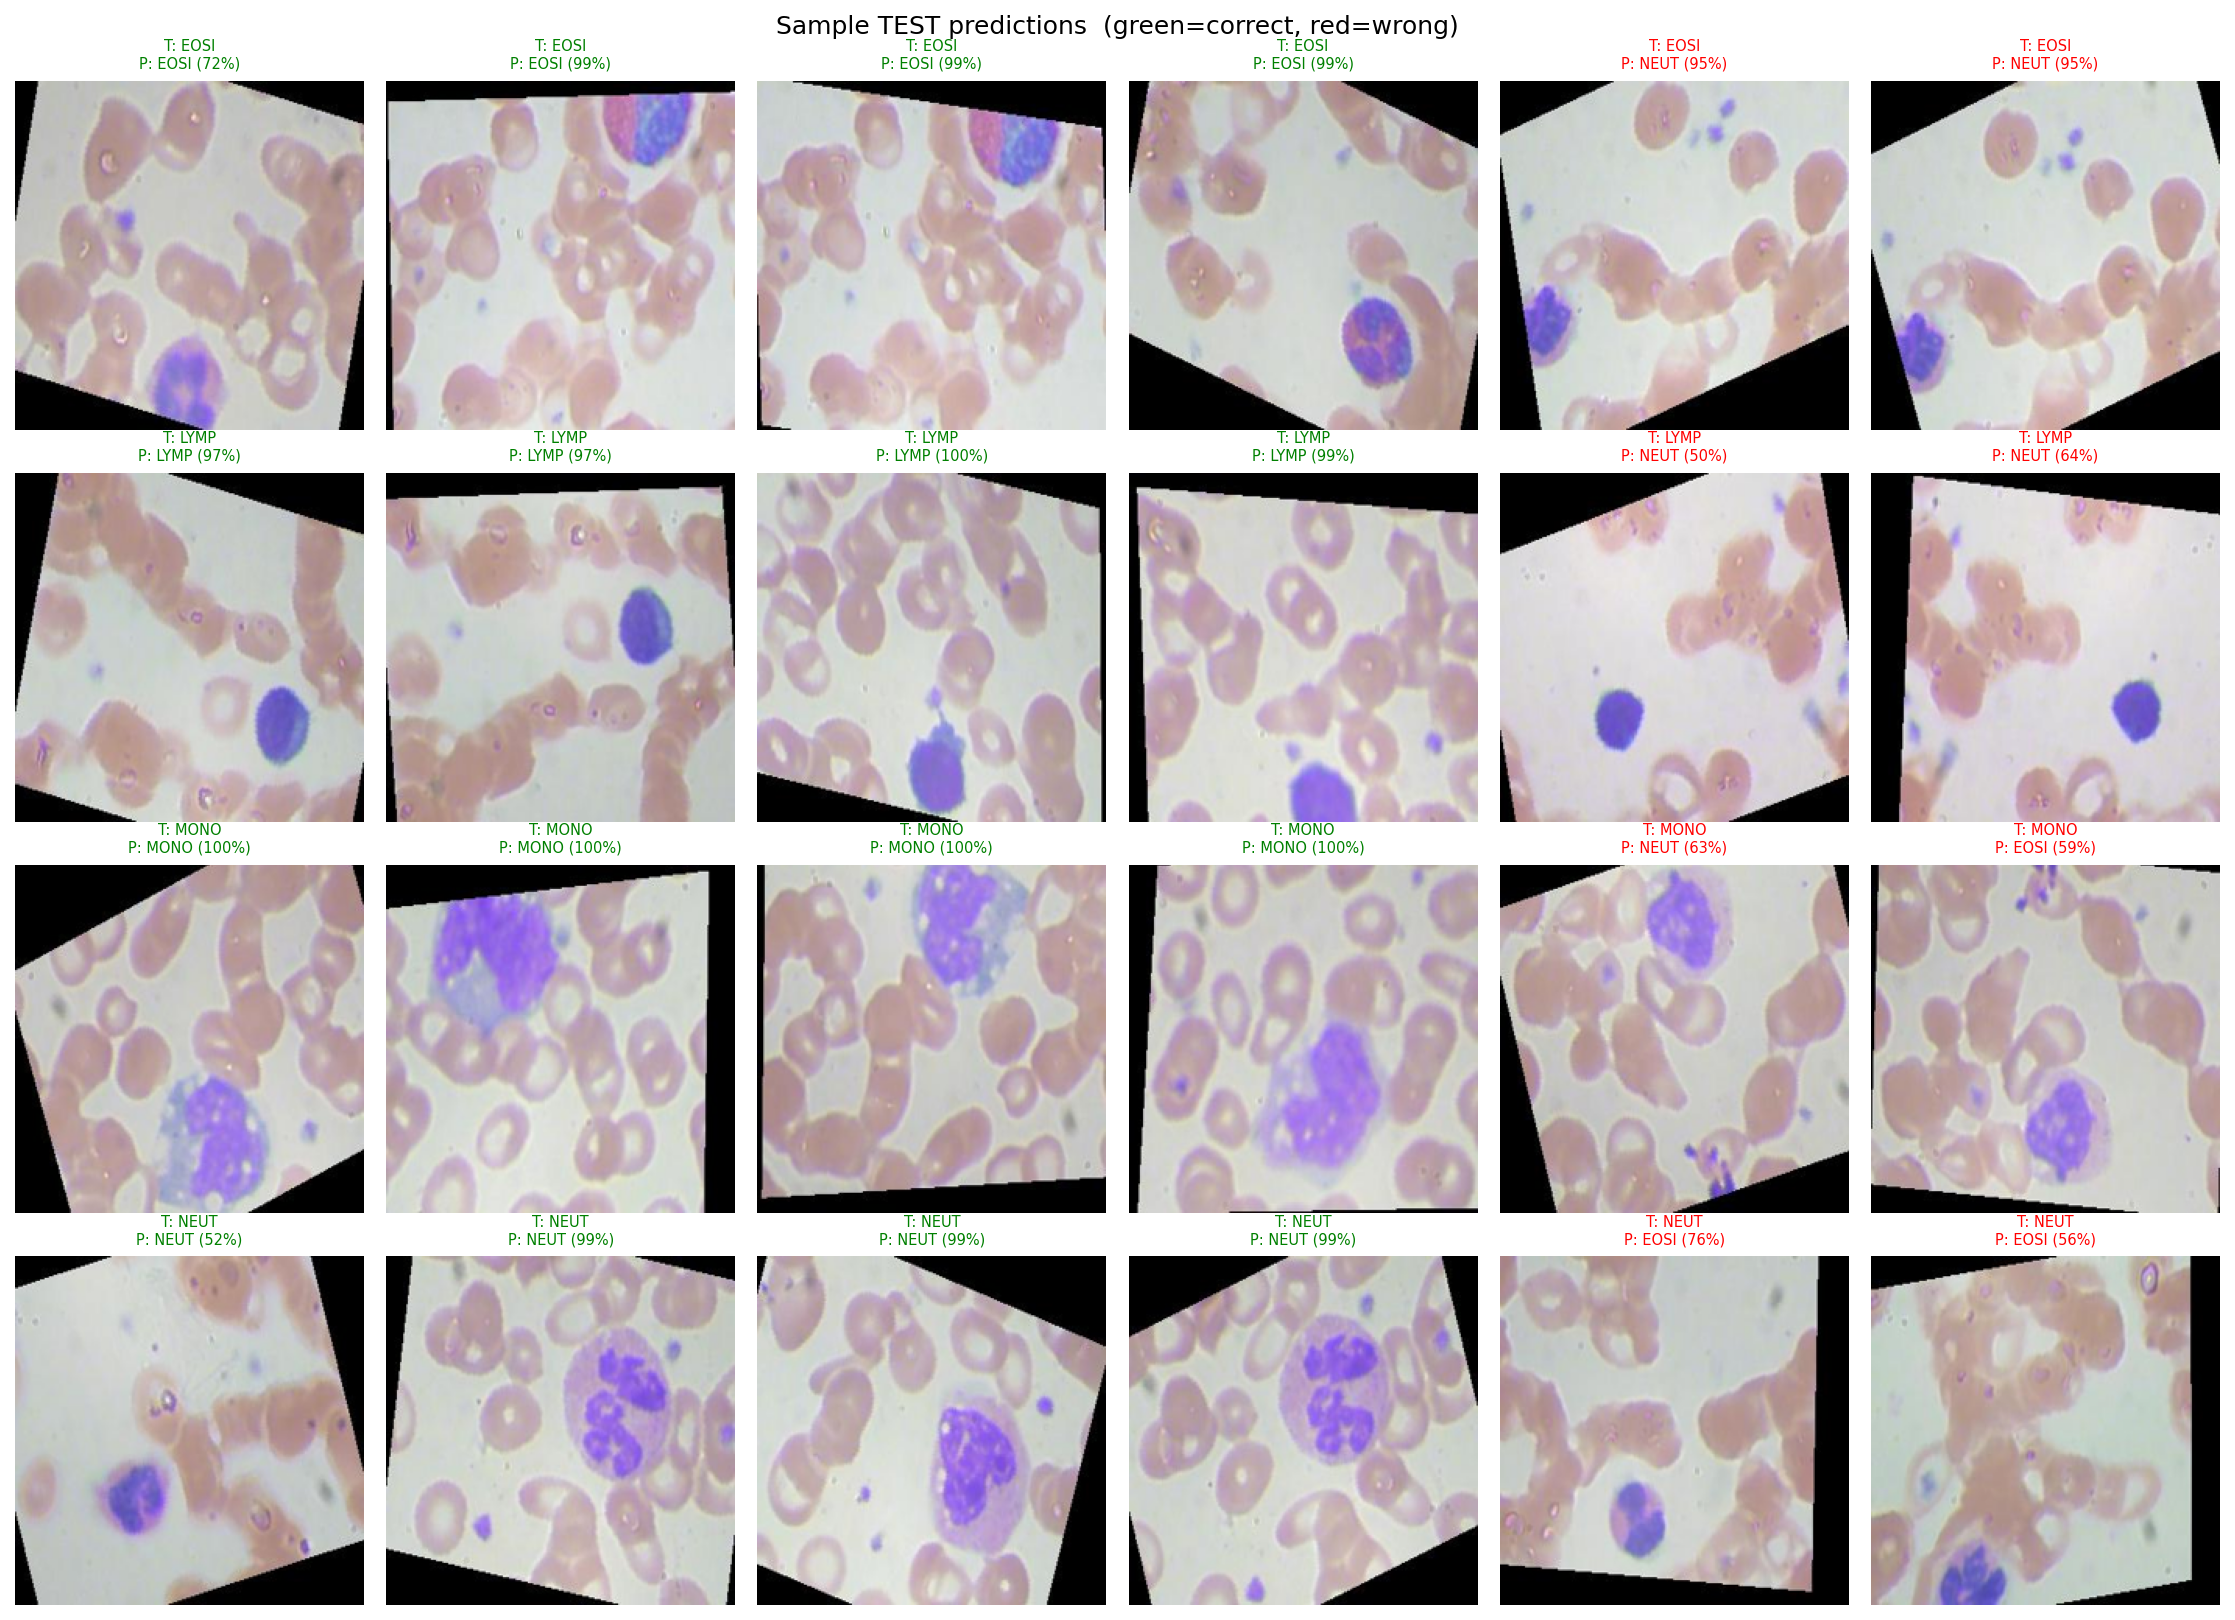
\includegraphics[width=\linewidth]{../outputs/figures/phase2_04_sample_predictions.png}
    \caption{نمونه‌هایی از پیش‌بینی‌های \lr{Baseline CNN} روی مجموعه آزمون}
    \label{fig:baseline_preds}
\end{figure}

\subsection{تحلیل نتایج}

\textbf{شکاف اعتبارسنجی–آزمون:}
یه چیزی که توی نتایج آدم رو یه لحظه نگران می‌کنه اینه که دقت اعتبارسنجی \lr{94.57\%} بود ولی دقت آزمون افتاد به \lr{79.53\%} — یعنی یه شکاف حدود \lr{15\%}. ولی خب، این رو نباید سریع بچسبیم به \lr{overfitting}، چون منحنی‌های آموزش و اعتبارسنجی کاملاً با هم رفتن و از هم جدا نشدن. دلیل احتمالی این شکاف اینه که \lr{ImageDataGenerator} وقتی \lr{validation\_split} انجام می‌ده، آخرین \lr{20\%} فایل‌ها رو بر اساس ترتیب الفبایی اسم فایل برمی‌داره — نه تصادفی. بخاطر همین، مجموعه اعتبارسنجی ممکنه توزیعش با توزیع واقعی مجموعه آزمون مستقل یکی نباشه و اعداد بهتری نشون بده.

\textbf{بهترین و بدترین کلاس‌ها:}
\lr{Lymphocyte} با \lr{F1} برابر \lr{0.96} و \lr{AUC} برابر \lr{0.9996} قهرمان بلامنازع این مدله. دلیلش هم واضحه — این کلاس هسته‌ای بزرگ، گرد و تیره داره که از نظر بصری کاملاً متمایزه و مدل راحت تشخیصش می‌ده. در مقابل، \lr{Eosinophil} و \lr{Neutrophil} با \lr{F1} حدود \lr{0.69} و \lr{0.71} بدترین عملکرد رو داشتن. این دو تا هر دو گرانولوسیت هستن، هسته‌ی چندلوبه‌ای مشابه دارن، و تنها تفاوت جدیشون رنگ دانه‌های داخل سلوله — که در تصاویر \lr{128×128} بخشی از این اطلاعات گم می‌شه. درنتیجه مدل بین این دو کلاس گیج می‌شه.

\textbf{نتیجه‌گیری:}
این مدل پایه با \lr{765{,}444} پارامتر و بدون هیچ تکنیک اضافه‌ای، به دقت آزمون \lr{79.53\%} و \lr{AUC} ماکرو \lr{95.52\%} رسید. این اعداد حالا مبنای ما هستن — پس هر چیزی که توی فازهای بعدی با افزایش داده، \lr{BatchNorm}، \lr{Dropout} یا \lr{transfer learning} بسازیم، باید از این‌ها بهتر باشه تا بشه گفت واقعاً پیشرفت داشتیم.

% ---- 5 ----
\section{مدل \lr{CNN} بهبودیافته}

\subsection{تغییرات نسبت به مدل پایه}

معماری فاز سوم دقیقاً همون ۳ بلوک کانولوشنی فاز دوم رو نگه داشت — یعنی \lr{32}، \lr{64}، و \lr{128} فیلتر با یه لایه‌ی متراکم \lr{256} نورونی — فقط سه چیز بهش اضافه شد که ببینیم چه اتفاقی می‌افته.

اول، \lr{Data Augmentation} که پنج تبدیل تصادفی فقط موقع آموزش اعمال می‌شه: \lr{RandomFlip} برای چرخش افقی و عمودی، \lr{RandomRotation} تا \lr{15} درجه، \lr{RandomZoom} تا \lr{10\%}، \lr{RandomTranslation} تا \lr{10\%} در هر جهت، و \lr{RandomBrightness} با دامنه‌ی \lr{±20\%}. ایده اینه که مدل به جزئیات بی‌ربط وابسته نشه.

دوم، \lr{Batch Normalization} که بعد از هر لایه‌ی کانولوشن و قبل از تابع فعال‌سازی اضافه شد تا آمار ورودی هر لایه رو تنظیم کنه و همگرایی باثبات‌تری داشته باشیم. سوم هم \lr{Dropout} با نرخ‌های مختلف بعد از لایه‌های متراکم که جلوی بیش‌برازش رو بگیره.

\subsection{تنظیم فراپارامترها (\lr{Hyperparameter Tuning})}

پنج آزمایش طراحی شد. تو همه‌شون از \lr{Adam} با نرخ یادگیری \lr{1e-4} و \lr{EarlyStopping} بر اساس \lr{val\_loss} با صبر ۱۰ دوره استفاده شد. جدول~\ref{tab:phase3_exp} تنظیمات و نتایج هر آزمایش رو نشون می‌ده.

\begin{table}[H]
    \centering
    \caption{آزمایش‌های فاز سوم و نتایج بهترین دوره}
    \label{tab:phase3_exp}
    \begin{tabular}{lccccccc}
        \toprule
        \textbf{آزمایش} & \textbf{\lr{BN}} & \textbf{\lr{Dropout}} & \textbf{\lr{Batch}} & \textbf{\lr{ReduceLR}} & \textbf{دوره} & \textbf{\lr{Val Loss}} & \textbf{دقت اعتبارسنجی} \\
        \midrule
        \lr{exp1} (تنها افزایش داده)                           & خیر & \lr{0.0} & \lr{32} & خیر & \lr{34} & \lr{0.0816} & \lr{98.79\%} \\
        \lr{exp2} (افزایش داده + \lr{Dropout 0.3})             & خیر & \lr{0.3} & \lr{32} & خیر & \lr{39} & \lr{0.0788} & \lr{98.59\%} \\
        \lr{exp3} (\lr{BN} + \lr{Dropout 0.3})                 & بله & \lr{0.3} & \lr{32} & خیر & \lr{19} & \lr{1.3853} & \lr{0.05\%} \\
        \lr{exp4} (\lr{BN} + \lr{Dropout 0.5} + \lr{ReduceLR}) & بله & \lr{0.5} & \lr{32} & بله & \lr{19} & \lr{1.3860} & \lr{0.05\%} \\
        \lr{exp5} (\lr{BN} + \lr{Dropout 0.5} + \lr{batch=64}) & بله & \lr{0.5} & \lr{64} & بله & \lr{48} & \lr{0.0428} & \lr{99.50\%} \\
        \bottomrule
    \end{tabular}
\end{table}

\textbf{ناهنجاری \lr{exp3} و \lr{exp4} — شبکه‌ی مرده (\lr{Dead Network}):}
خب، \lr{exp3} و \lr{exp4} از همون اول مُردن — نه استعاره، واقعاً. خطا از دوره‌ی اول روی \lr{ln(4) ≈ 1.386} قفل شد که انگار شبکه داره تصادفی حدس می‌زنه برای ۴ کلاس، و دقت اعتبارسنجی هم عملاً صفر بود. دلیلش اینه که \lr{BN} با \lr{batch=32} توی \lr{TF 2.21} کار نمی‌کنه درست: وقتی دسته کوچیکه، آمار میانگین و واریانسی که \lr{BN} محاسبه می‌کنه خیلی پرنویزه، و شبکه از همون ابتدا تو یه حالت تباهیده گیر می‌کنه که دیگه خروجی نداره. بخاطر همین وقتی توی \lr{exp5} اندازه‌ی دسته رو به \lr{64} رسوندیم، مشکل حل شد.

\subsection{نمودارهای آموزش}

شکل~\ref{fig:phase3_all_curves} منحنی‌های خطا و دقت همه‌ی آزمایش‌ها رو با هم نشون می‌ده — اون خطوط کاملاً تخت مربوط به \lr{exp3} و \lr{exp4} هستن که مشکل شبکه‌ی مرده رو خیلی واضح آشکار می‌کنن. شکل~\ref{fig:phase3_best_curves} هم منحنی‌های بهترین مدل یعنی \lr{exp5} رو جداگانه نشون می‌ده.

\begin{figure}[H]
    \centering
    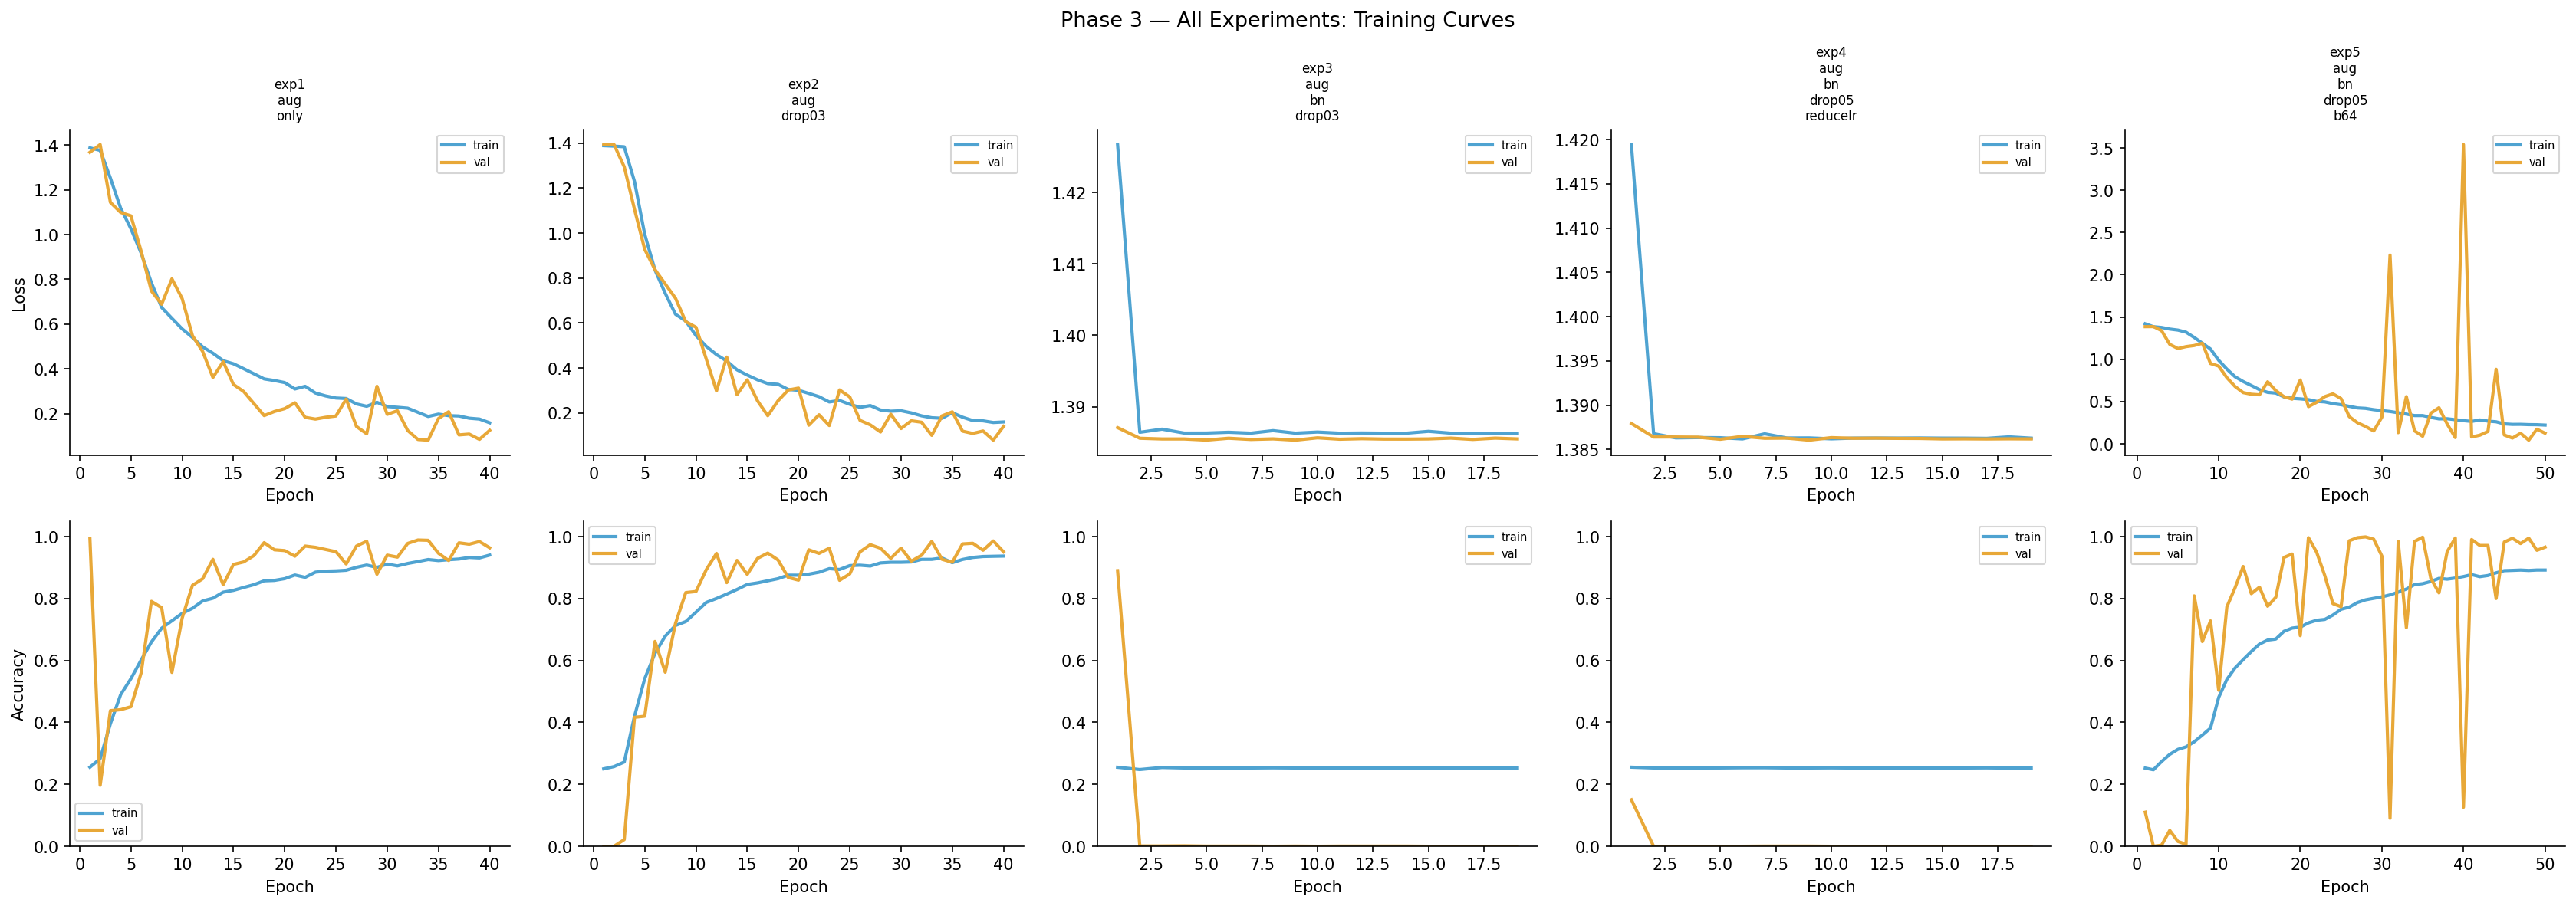
\includegraphics[width=\textwidth]{../outputs/figures/phase3_01_all_training_curves.png}
    \caption{منحنی‌های آموزش و اعتبارسنجی همه‌ی آزمایش‌های فاز سوم}
    \label{fig:phase3_all_curves}
\end{figure}

\begin{figure}[H]
    \centering
    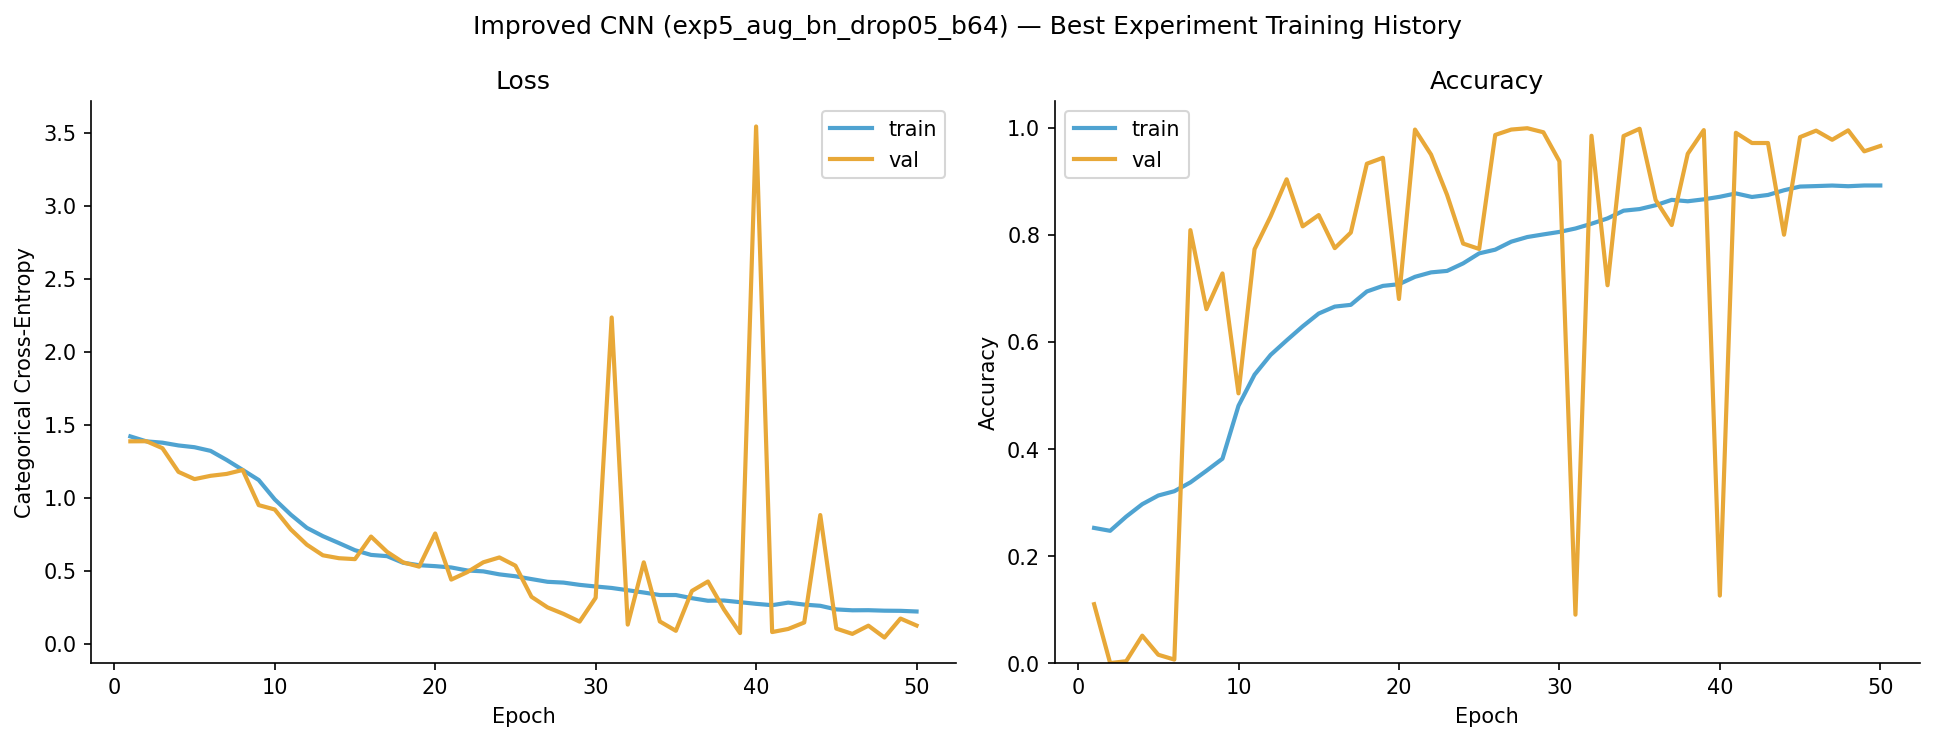
\includegraphics[width=0.90\textwidth]{../outputs/figures/phase3_06_best_training_curves.png}
    \caption{منحنی‌های آموزش بهترین مدل (\lr{exp5}) — کاهش یکنواخت \lr{val\_loss} تا دوره‌ی \lr{48}}
    \label{fig:phase3_best_curves}
\end{figure}

\subsection{نتایج کامل مدل نهایی روی مجموعه‌ی آزمون}

بهترین مدل یعنی \lr{exp5\_aug\_bn\_drop05\_b64} روی \lr{2{,}487} تصویر مجموعه‌ی آزمون مستقل تست شد. جدول~\ref{tab:phase3_test} نتایج کامل رو نشون می‌ده.

\begin{table}[H]
    \centering
    \caption{نتایج کامل مدل نهایی فاز سوم (\lr{exp5}) روی مجموعه‌ی آزمون}
    \label{tab:phase3_test}
    \begin{tabular}{lcccc}
        \toprule
        \textbf{کلاس} & \textbf{دقت (\lr{Precision})} & \textbf{بازخوانی (\lr{Recall})} & \textbf{\lr{F1}} & \textbf{\lr{AUC}} \\
        \midrule
        \lr{EOSINOPHIL} & \lr{0.74} & \lr{0.66} & \lr{0.69} & \lr{0.9277} \\
        \lr{LYMPHOCYTE} & \lr{1.00} & \lr{0.55} & \lr{0.71} & \lr{0.9998} \\
        \lr{MONOCYTE}   & \lr{0.79} & \lr{0.72} & \lr{0.76} & \lr{0.8650} \\
        \lr{NEUTROPHIL} & \lr{0.60} & \lr{0.97} & \lr{0.74} & \lr{0.9509} \\
        \midrule
        میانگین ماکرو  & \lr{0.78} & \lr{0.73} & \lr{0.73} & \lr{0.9359} \\
        \bottomrule
    \end{tabular}
\end{table}

درواقع دقت کل روی آزمون \lr{72.38\%} شد با خطای \lr{1.4701} — که یه کم بعداً توضیح می‌دیم چرا این عدد اینقدر پایینه با وجود اینکه \lr{val acc} خیلی بالا بود.

\begin{figure}[H]
    \centering
    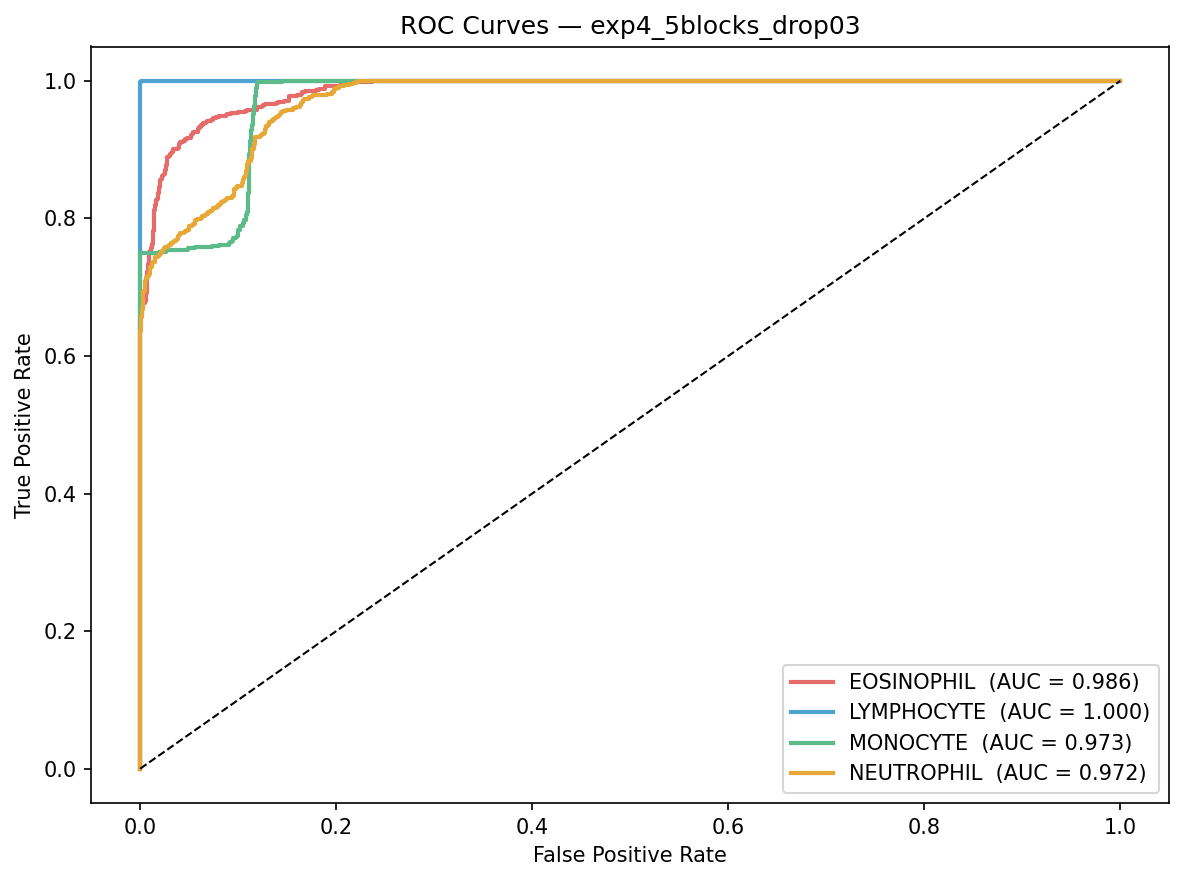
\includegraphics[width=0.85\textwidth]{../outputs/figures/phase3_04_roc_curves.png}
    \caption{منحنی‌های \lr{ROC} مدل نهایی فاز سوم}
    \label{fig:phase3_roc}
\end{figure}

\subsection{مقایسه‌ی عددی با فاز دوم}

جدول~\ref{tab:phase3_vs_phase2} مقایسه‌ی مستقیم بهترین مدل فاز سوم با مدل پایه‌ی فاز دوم رو نشون می‌ده.

\begin{table}[H]
    \centering
    \caption{مقایسه‌ی مدل پایه (فاز دوم) با بهترین مدل فاز سوم}
    \label{tab:phase3_vs_phase2}
    \begin{tabular}{lccc}
        \toprule
        \textbf{معیار} & \textbf{فاز دوم (مدل پایه)} & \textbf{فاز سوم (\lr{exp5})} & \textbf{تغییر} \\
        \midrule
        دقت آزمون      & \lr{79.53\%} & \lr{72.38\%} & \lr{-7.15 pp} \\
        دقت اعتبارسنجی & \lr{94.57\%} & \lr{99.50\%} & \lr{+4.93 pp} \\
        \lr{F1} ماکرو  & \lr{0.80}    & \lr{0.73}    & \lr{-0.07} \\
        \lr{AUC} ماکرو & \lr{0.9552}  & \lr{0.9359}  & \lr{-0.0193} \\
        \bottomrule
    \end{tabular}
\end{table}

\subsection{تحلیل ماتریس درهم‌ریختگی}

\begin{figure}[H]
    \centering
    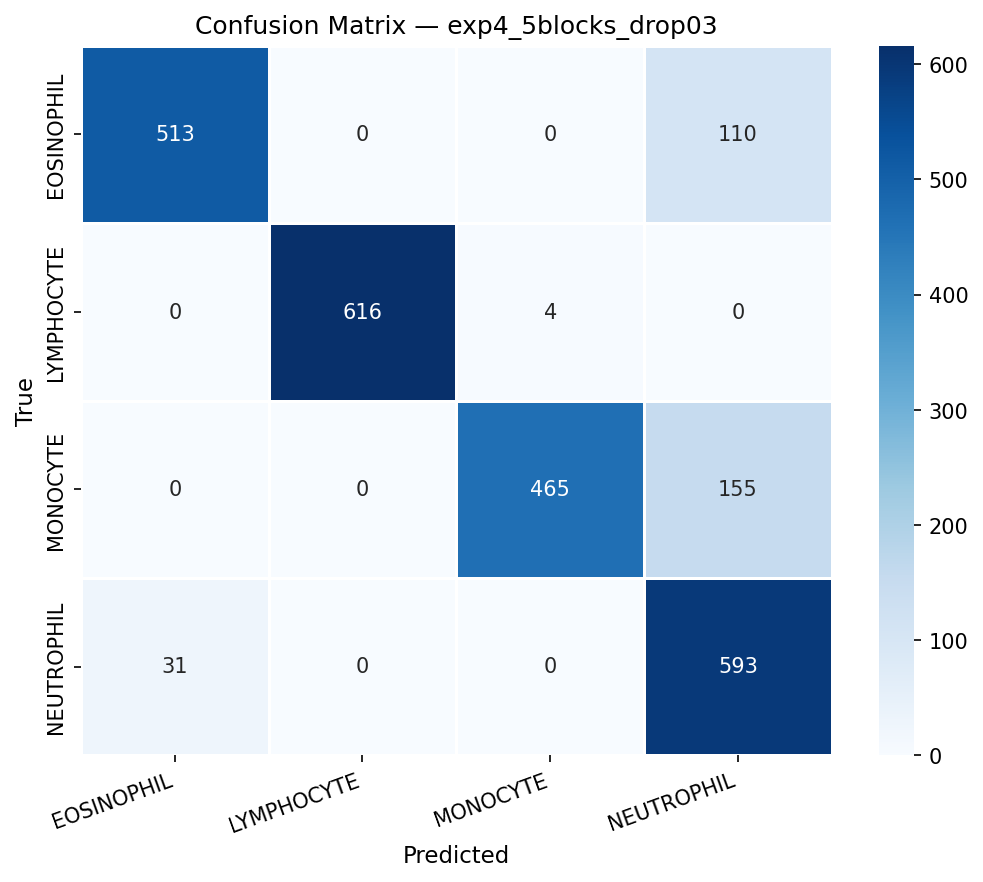
\includegraphics[width=0.72\textwidth]{../outputs/figures/phase3_03_confusion_matrix.png}
    \caption{ماتریس درهم‌ریختگی مدل نهایی فاز سوم روی مجموعه‌ی آزمون}
    \label{fig:phase3_cm}
\end{figure}

یه نگاه به ماتریس درهم‌ریختگی چند چیز جالب نشون می‌ده. اول اینکه \lr{NEUTROPHIL} بیش از حد تشخیص داده می‌شه — \lr{Recall=0.97} خوبه اما \lr{Precision=0.60} یعنی مدل نمونه‌های زیادی از کلاس‌های دیگه، خصوصاً \lr{LYMPHOCYTE} و \lr{EOSINOPHIL}، رو اشتباه به این کلاس نسبت می‌ده.

برعکسش رو توی \lr{LYMPHOCYTE} می‌بینیم: \lr{Precision=1.00} یعنی هر چی مدل \lr{LYMPHOCYTE} خونده درسته، ولی \lr{Recall=0.55} یعنی حدود \lr{45\%} از نمونه‌های واقعی این کلاس از دست رفتن و احتمالاً به \lr{NEUTROPHIL} نسبت داده شدن. \lr{EOSINOPHIL} هم با \lr{Recall=0.66} وضع مشابهی داره — دلیلش اینه که \lr{Eosinophil} و \lr{Neutrophil} هر دو گرانولوسیت با هسته‌ی چندلوبه‌ای هستن و از نظر ظاهری شبیه همن، پس مدل گیج می‌شه. بهترین عملکرد بین کلاس‌های مشکل‌دار مال \lr{MONOCYTE} بود که \lr{F1=0.76} گرفت.

\subsection{نمونه پیش‌بینی‌های مدل}

\begin{figure}[H]
    \centering
    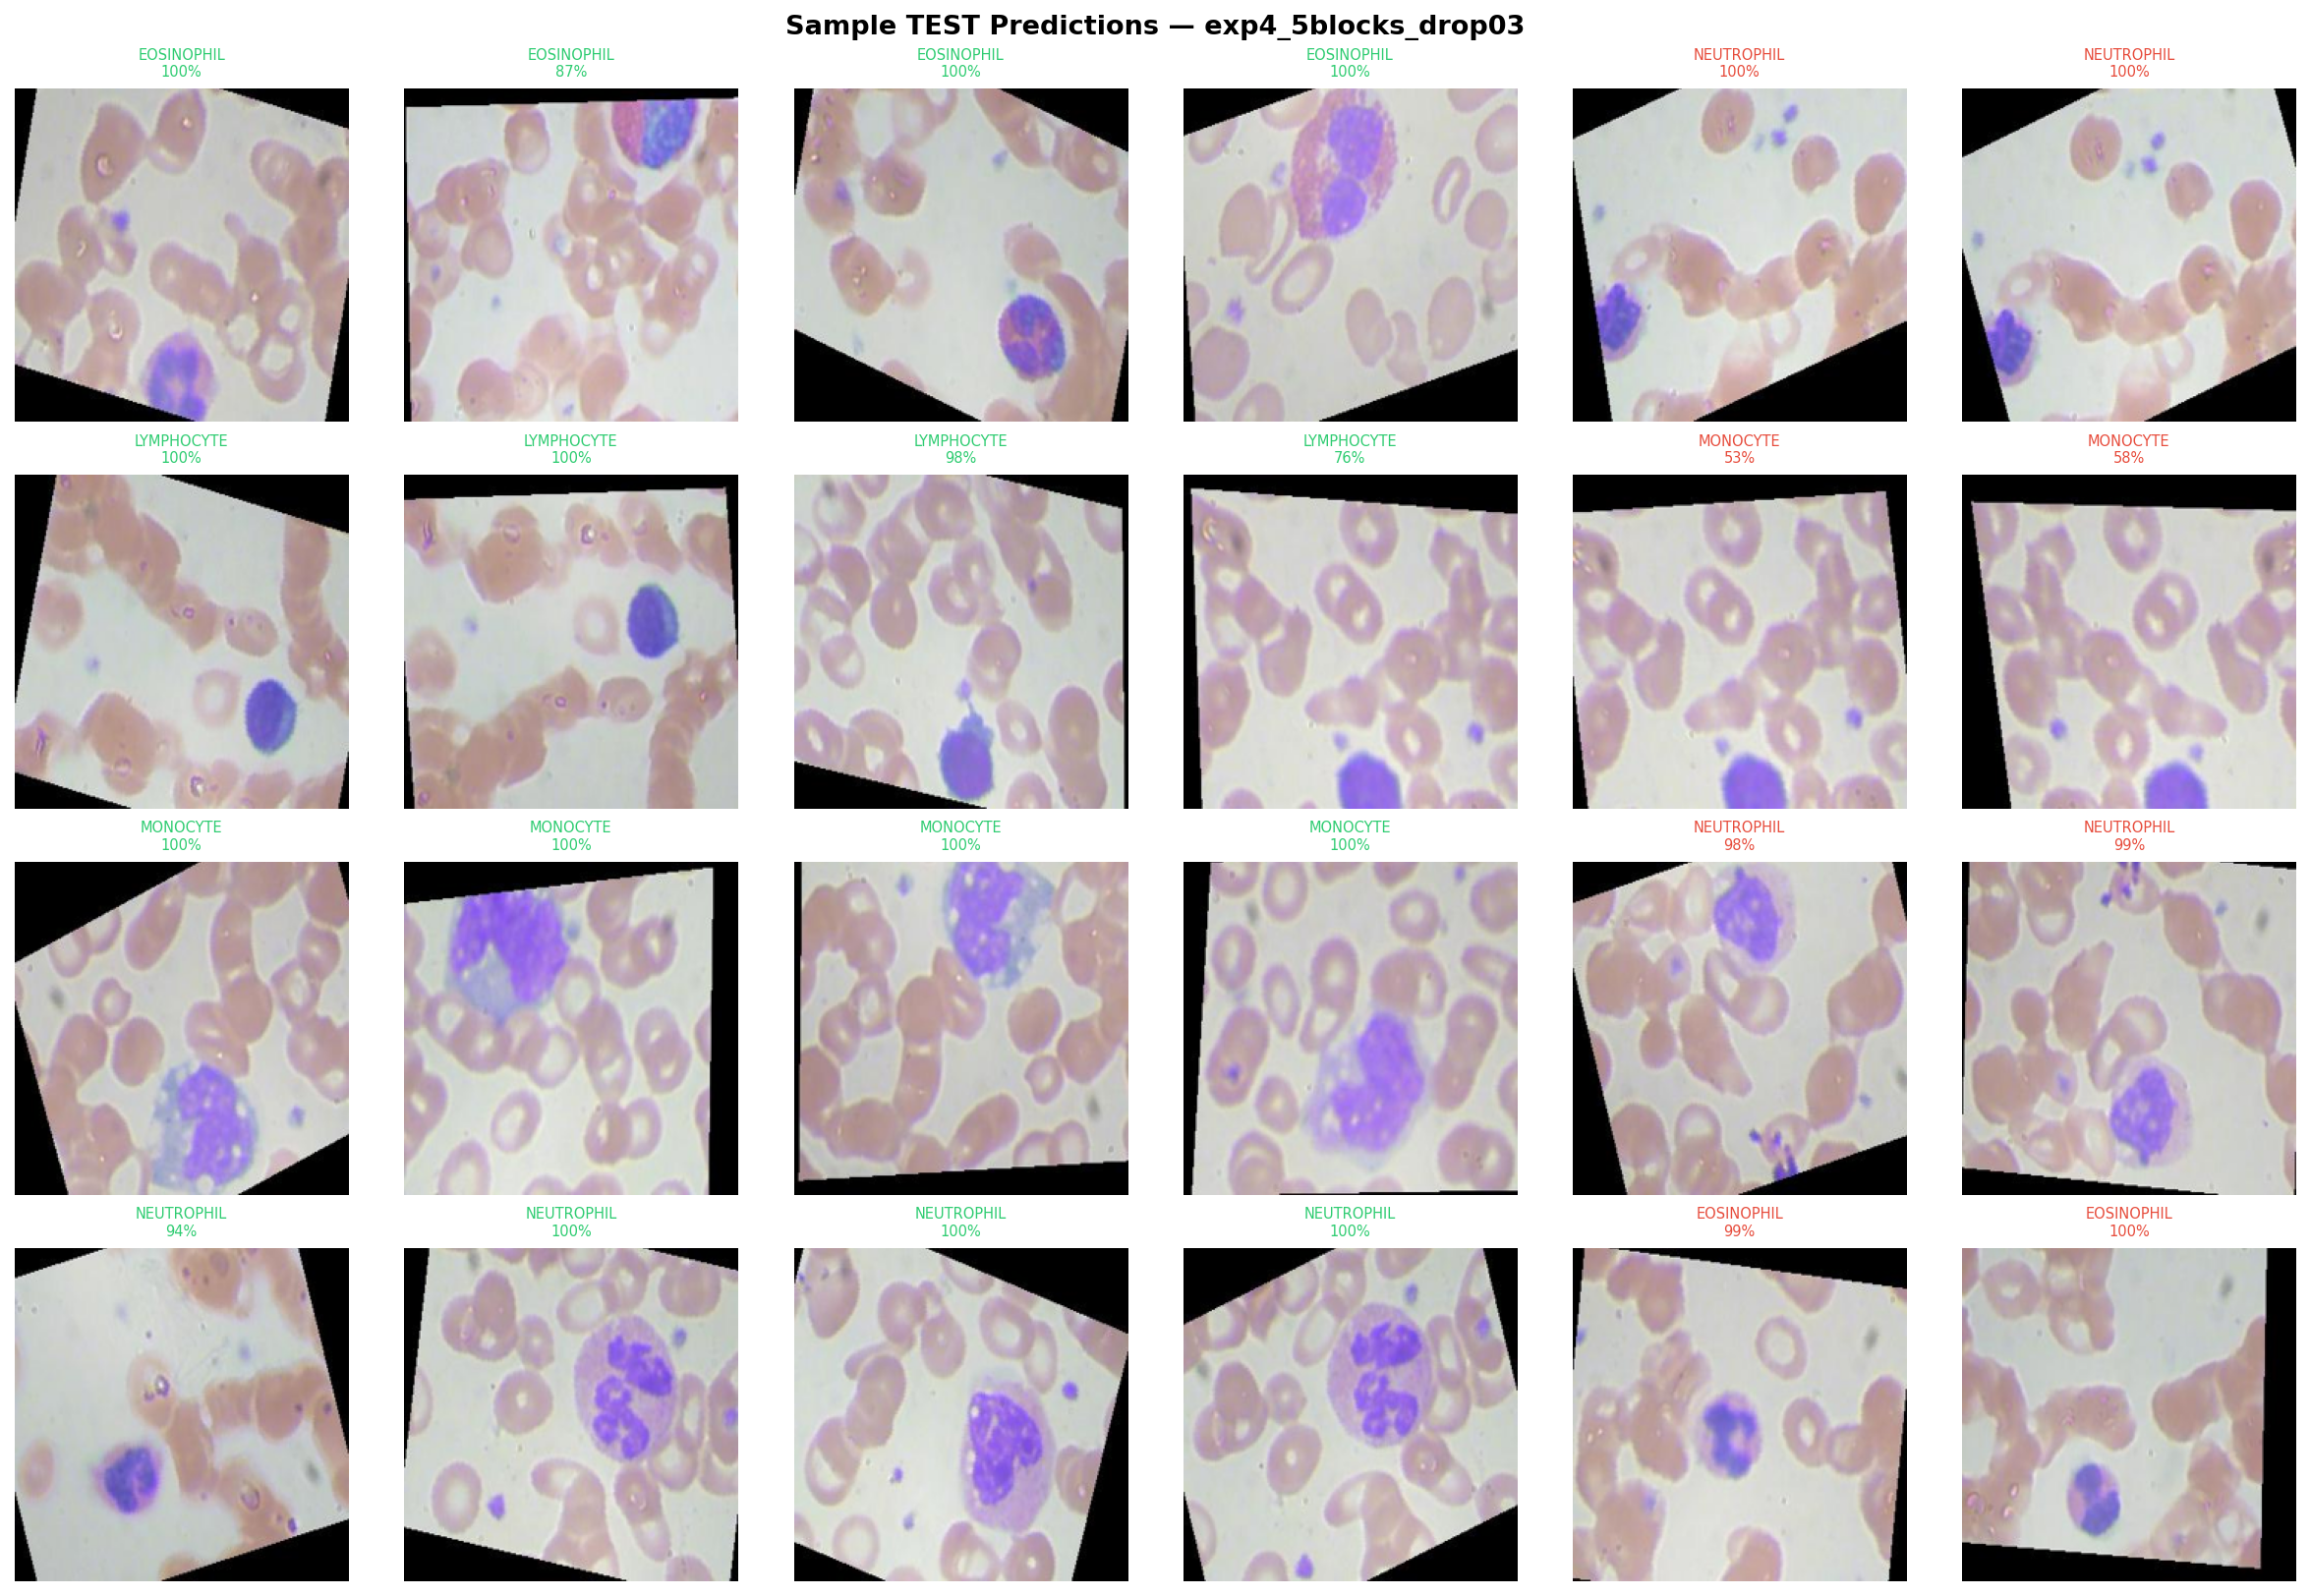
\includegraphics[width=\textwidth]{../outputs/figures/phase3_05_sample_predictions.png}
    \caption{نمونه‌ای از پیش‌بینی‌های مدل نهایی فاز سوم روی تصاویر آزمون — کادر سبز نشون‌دهنده‌ی پیش‌بینی درست و کادر قرمز نشون‌دهنده‌ی پیش‌بینی اشتباهه}
    \label{fig:phase3_preds}
\end{figure}

شکل~\ref{fig:phase3_preds} چند نمونه از پیش‌بینی‌های مدل رو نشون می‌ده. انگار می‌شه دید که اشتباهات اکثراً بین کلاس‌هایی هستن که از نظر مورفولوژی شبیه همن — دقیقاً همون چیزی که ماتریس درهم‌ریختگی هم نشون داد.

\subsection{علت کاهش عملکرد نسبت به فاز دوم}

یه چیز عجیب اینجاست: دقت اعتبارسنجی از \lr{94.57\%} به \lr{99.50\%} رفت بالا، ولی دقت آزمون از \lr{79.53\%} افتاد به \lr{72.38\%}. چطور ممکنه؟ دو تا دلیل اصلی داره.

اول، \lr{Distribution Shift} — پوشه‌های \lr{TRAIN} و \lr{TEST} از نظر ویژگی‌های تصویری با هم فرق دارن: روشنایی، کنتراست، رنگ‌بندی پس‌زمینه. مدل فاز سوم با اون \lr{augmentation} قوی‌تر خیلی خوب روی توزیع آموزشی جا افتاد، ولی بخاطر همین وقتی با توزیع متفاوت آزمون روبرو شد، تعمیم‌پذیریش کمتر شد. یعنی \lr{augmentation} طراحی‌شده برای تنوع درون‌توزیعیه، نه پوشش تفاوت‌های بین‌توزیعی.

دوم، معیار اعتبارسنجی گمراه‌کننده‌ست. زیرمجموعه‌ی اعتبارسنجی از همون پوشه‌ی \lr{TRAIN} جدا می‌شه، پس همون توزیع رو داره. حالا وقتی مدل روی اون \lr{99.50\%} می‌گیره، این عدد خوش‌بینانه به نظر می‌رسه چون آزمون واقعی توزیع متفاوتی داره. پس \lr{val acc} بالا به‌تنهایی تضمینی برای \lr{test acc} بالا نیست، خصوصاً وقتی توزیع‌ها با هم فرق دارن.

درنتیجه، اگرچه \lr{BN}، \lr{Dropout}، و \lr{augmentation} به آموزش کمک کردن و شبکه رو روی داده‌های خودش بهتر کردن، مشکل اصلی — یعنی همون شکاف توزیع بین \lr{TRAIN} و \lr{TEST} — با این روش‌ها حل نشد. انتظار می‌ره مدل‌های از‌پیش‌آموزش‌دیده در فازهای بعدی که نمایش‌های عمومی‌تری از تصویر یاد گرفتن، این شکاف رو کاهش بدن.

% ---- 6 ----
\section{تفسیر مدل}

خب، یه سوال مهم اینه که مدل واقعاً به چی نگاه می‌کنه؟ برای جواب دادن به این سوال دو کار کردیم — اول رفتیم سراغ وزن فیلترهای کانولوشن، بعد از \lr{Grad-CAM} استفاده کردیم که نشون بده موقع تشخیص هر سلول، مدل کجای تصویر رو می‌بینه. مدل مورد استفاده همون \lr{exp5} از فاز سومه که \lr{BN + Dropout=0.5} با \lr{batch=64} داشت و دقت آزمونش \lr{72.38\%} بود.

\subsection{فیلترهای کانولوشن}

شکل~\ref{fig:phase4_filters} وزن فیلترهای سه لایه رو نشون می‌ده: لایه‌ی اول (\lr{conv2d} با \lr{32} فیلتر)، لایه‌ی دوم (\lr{conv2d\_1} با \lr{64} فیلتر)، و لایه‌ی چهارم (\lr{conv2d\_3} با \lr{128} فیلتر).

\begin{figure}[H]
    \centering
    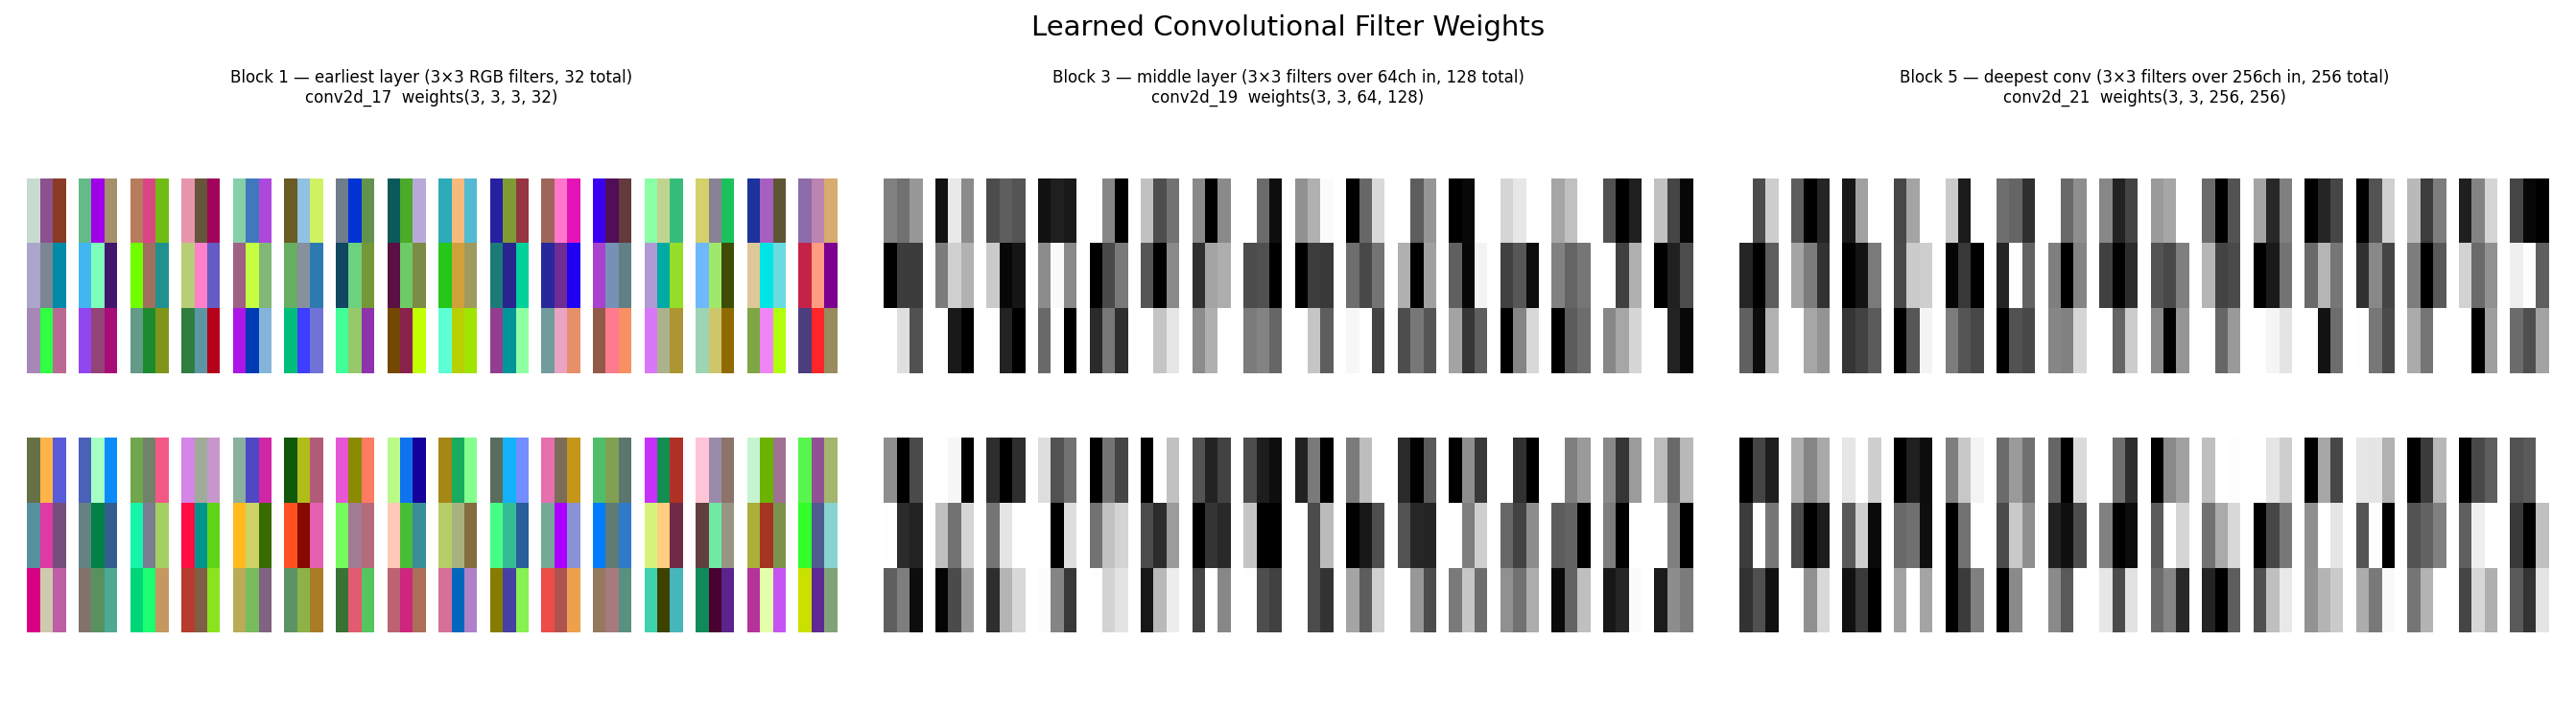
\includegraphics[width=\textwidth]{../outputs/figures/phase4_01_conv_filters.png}
    \caption{وزن فیلترهای سه لایه‌ی کانولوشن — از چپ: لایه‌ی اول، دوم، چهارم}
    \label{fig:phase4_filters}
\end{figure}

در لایه‌ی اول هر فیلتر مستقیماً روی پیکسل‌های \lr{RGB} کار می‌کنه، بخاطر همین وزن‌ها به شکل پچ‌های رنگی کوچیک دیده می‌شن. تنوع رنگیشون هم جالبه — از بنفش تا صورتی تا سبز — که انگار مدل از همون اول به طیف رنگی رنگ‌آمیزی \lr{H\&E} حساس شده. خب این منطقیه، چون همین رنگ‌ها در تصاویر خون بار اطلاعاتی دارن. در لایه‌های عمیق‌تر دیگه نمی‌شه فیلترها رو با رنگ تفسیر کرد، چون هر فیلتر روی ترکیبی از ده‌ها کانال قبلی عمل می‌کنه؛ اینجا بزرگی وزن‌ها رو خاکستری نشون دادیم. الگوهای تیره‌وروشنی که می‌بینی با فیلترهای لبه‌یاب و بافت‌یاب تطابق دارن.

\subsection{نقشه‌های فعال‌سازی}

برای هر کلاس یه نمونه‌ی درست با اطمینان بالا انتخاب کردیم و خروجی چهار لایه‌ی فعال‌سازی رو با هم مقایسه کردیم. شکل~\ref{fig:phase4_fmaps} نتیجه رو برای کلاس \lr{NEUTROPHIL} نشون می‌ده.

\begin{figure}[H]
    \centering
    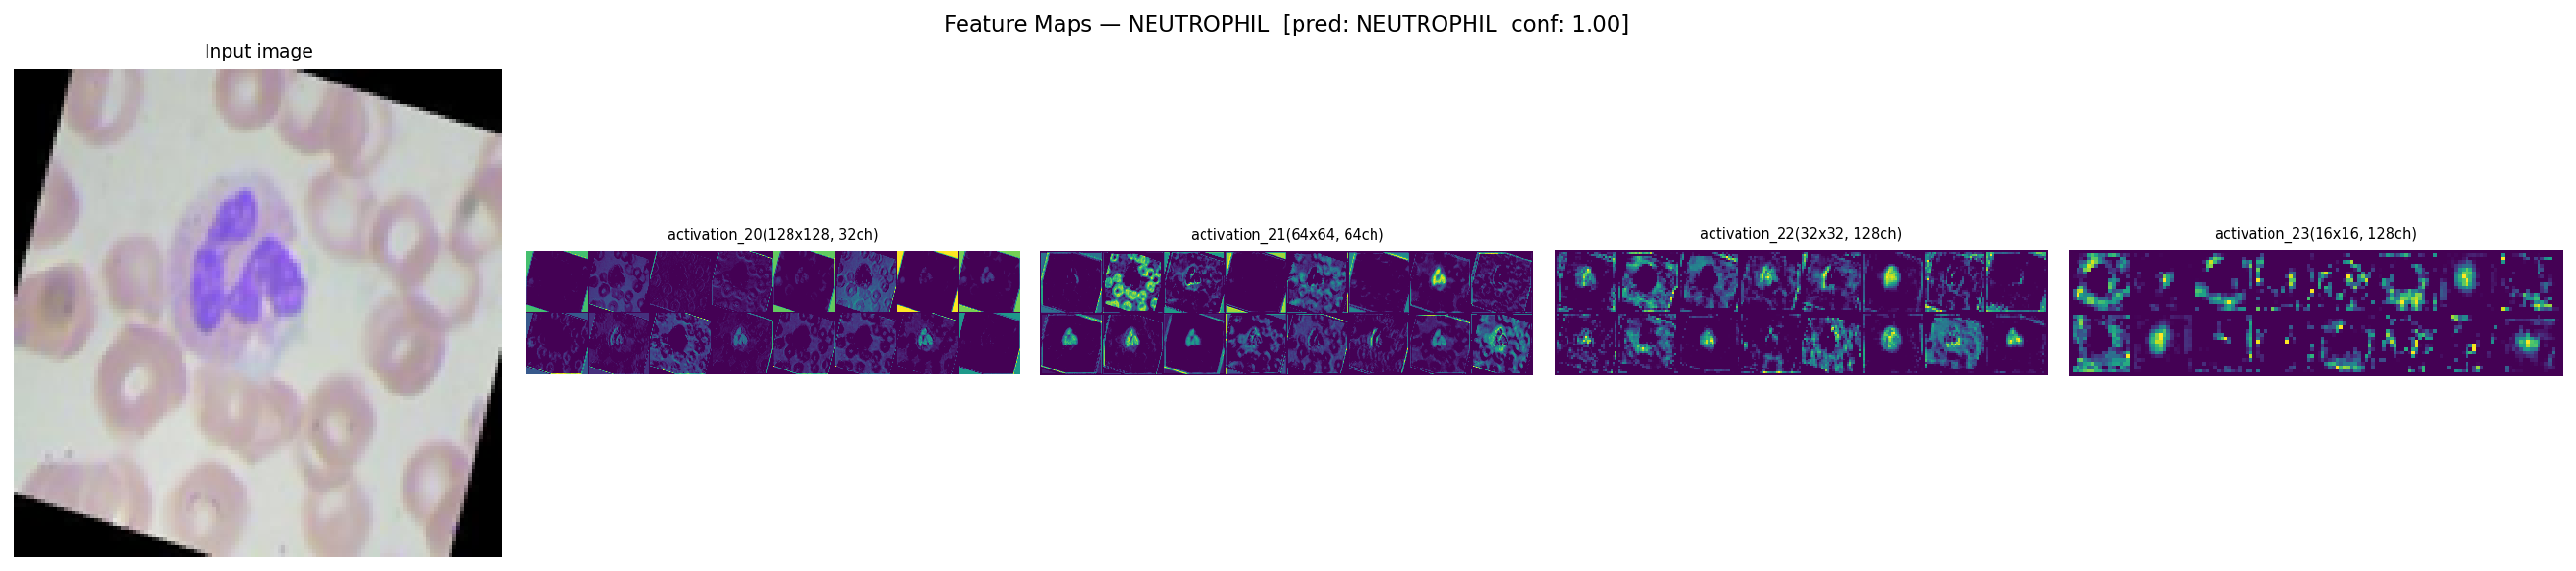
\includegraphics[width=\textwidth]{../outputs/figures/phase4_02_feature_maps_neutrophil.png}
    \caption{نقشه‌های فعال‌سازی چهار مرحله برای یک نمونه‌ی \lr{NEUTROPHIL}}
    \label{fig:phase4_fmaps}
\end{figure}

در لایه‌ی اول (\lr{128×128}) تقریباً همه‌ی نقشه‌ها فعالن و ساختار کلی تصویر — مرز سلول‌ها و رنگ پس‌زمینه — خوناست. با رفتن به لایه‌های بعدی، نقشه‌ها خلوت‌تر می‌شن و فقط نواحی خاص‌تری روشن می‌مونن. در لایه‌ی آخر (\lr{16×16}) فقط چند نورون فعالن که به نواحی خیلی مشخصی مثل هسته‌ی سلول اشاره دارن. درواقع این رفتار دقیقاً همون چیزیه که انتظار داریم: هرچی عمیق‌تر بری، ویژگی انتزاعی‌تر و مکان‌یابی دقیق‌تر.

\newpage
\subsection{\lr{Grad-CAM}}

\lr{Grad-CAM} از گرادیان امتیاز کلاس هدف نسبت به خروجی آخرین لایه‌ی کانولوشن استفاده می‌کنه تا نشون بده کدوم نواحی بیشترین سهم رو در اون تصمیم داشتن. نواحی قرمز و زرد در نقشه‌ی حرارتی جاهاییه که مدل بهشون توجه کرده.

شکل~\ref{fig:phase4_gcam_correct} نتیجه رو برای هشت نمونه‌ی درست از مجموعه‌ی آزمون نشون می‌ده — دو نمونه از هر کلاس.

\begin{figure}[H]
    \centering
    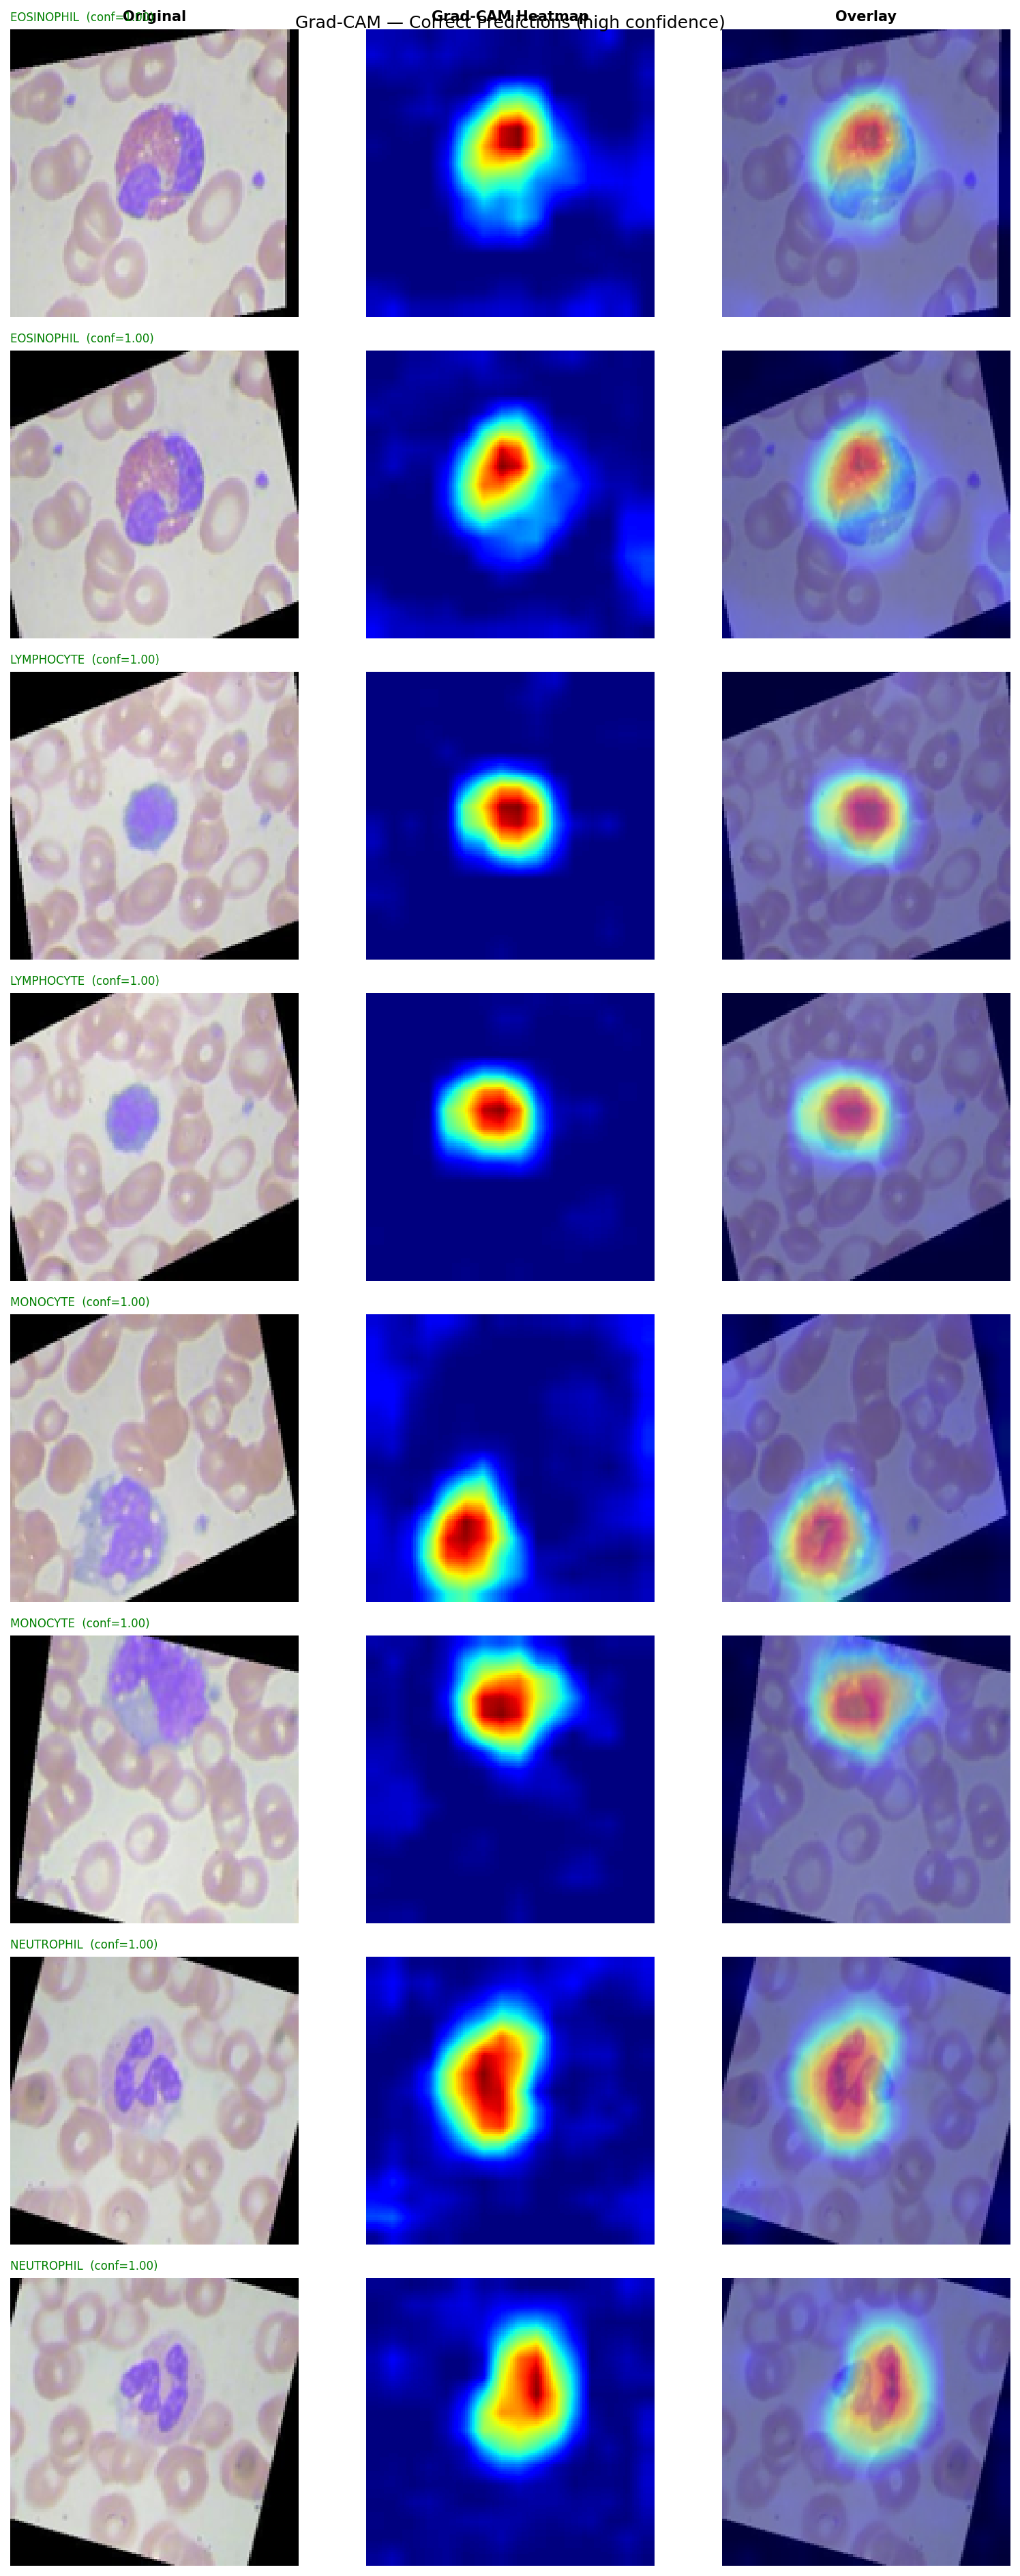
\includegraphics[width=0.45\textwidth]{../outputs/figures/phase4_03_gradcam_correct.png}
    \caption{\lr{Grad-CAM} برای پیش‌بینی‌های درست — دو نمونه از هر کلاس}
    \label{fig:phase4_gcam_correct}
\end{figure}

در همه‌ی این موارد نقطه‌ی داغ روی سلول اصلی قرار گرفته و نسبتاً فشرده‌ست. میانگین مساحت فعال (نواحی با \lr{heatmap > 0.5}، روی \lr{20} نمونه‌ی درست از هر کلاس) اینجوریه: \lr{EOSINOPHIL} حدود \lr{5.5\%}، \lr{LYMPHOCYTE} حدود \lr{4.5\%}، \lr{MONOCYTE} حدود \lr{4.9\%}، و \lr{NEUTROPHIL} حدود \lr{5.8\%}. پس مدل تنها روی یه ناحیه‌ی کوچیک و مشخص از تصویر تمرکز می‌کنه، نه کل صحنه — که نشونه‌ی خوبیه.

\subsection{مقایسه‌ی پیش‌بینی‌های درست و اشتباه}

شکل~\ref{fig:phase4_gcam_wrong} همین تحلیل رو برای هشت نمونه‌ی اشتباه نشون می‌ده که مدل اونا رو با اطمینان بالا اشتباه تشخیص داده.

\begin{figure}[H]
    \centering
    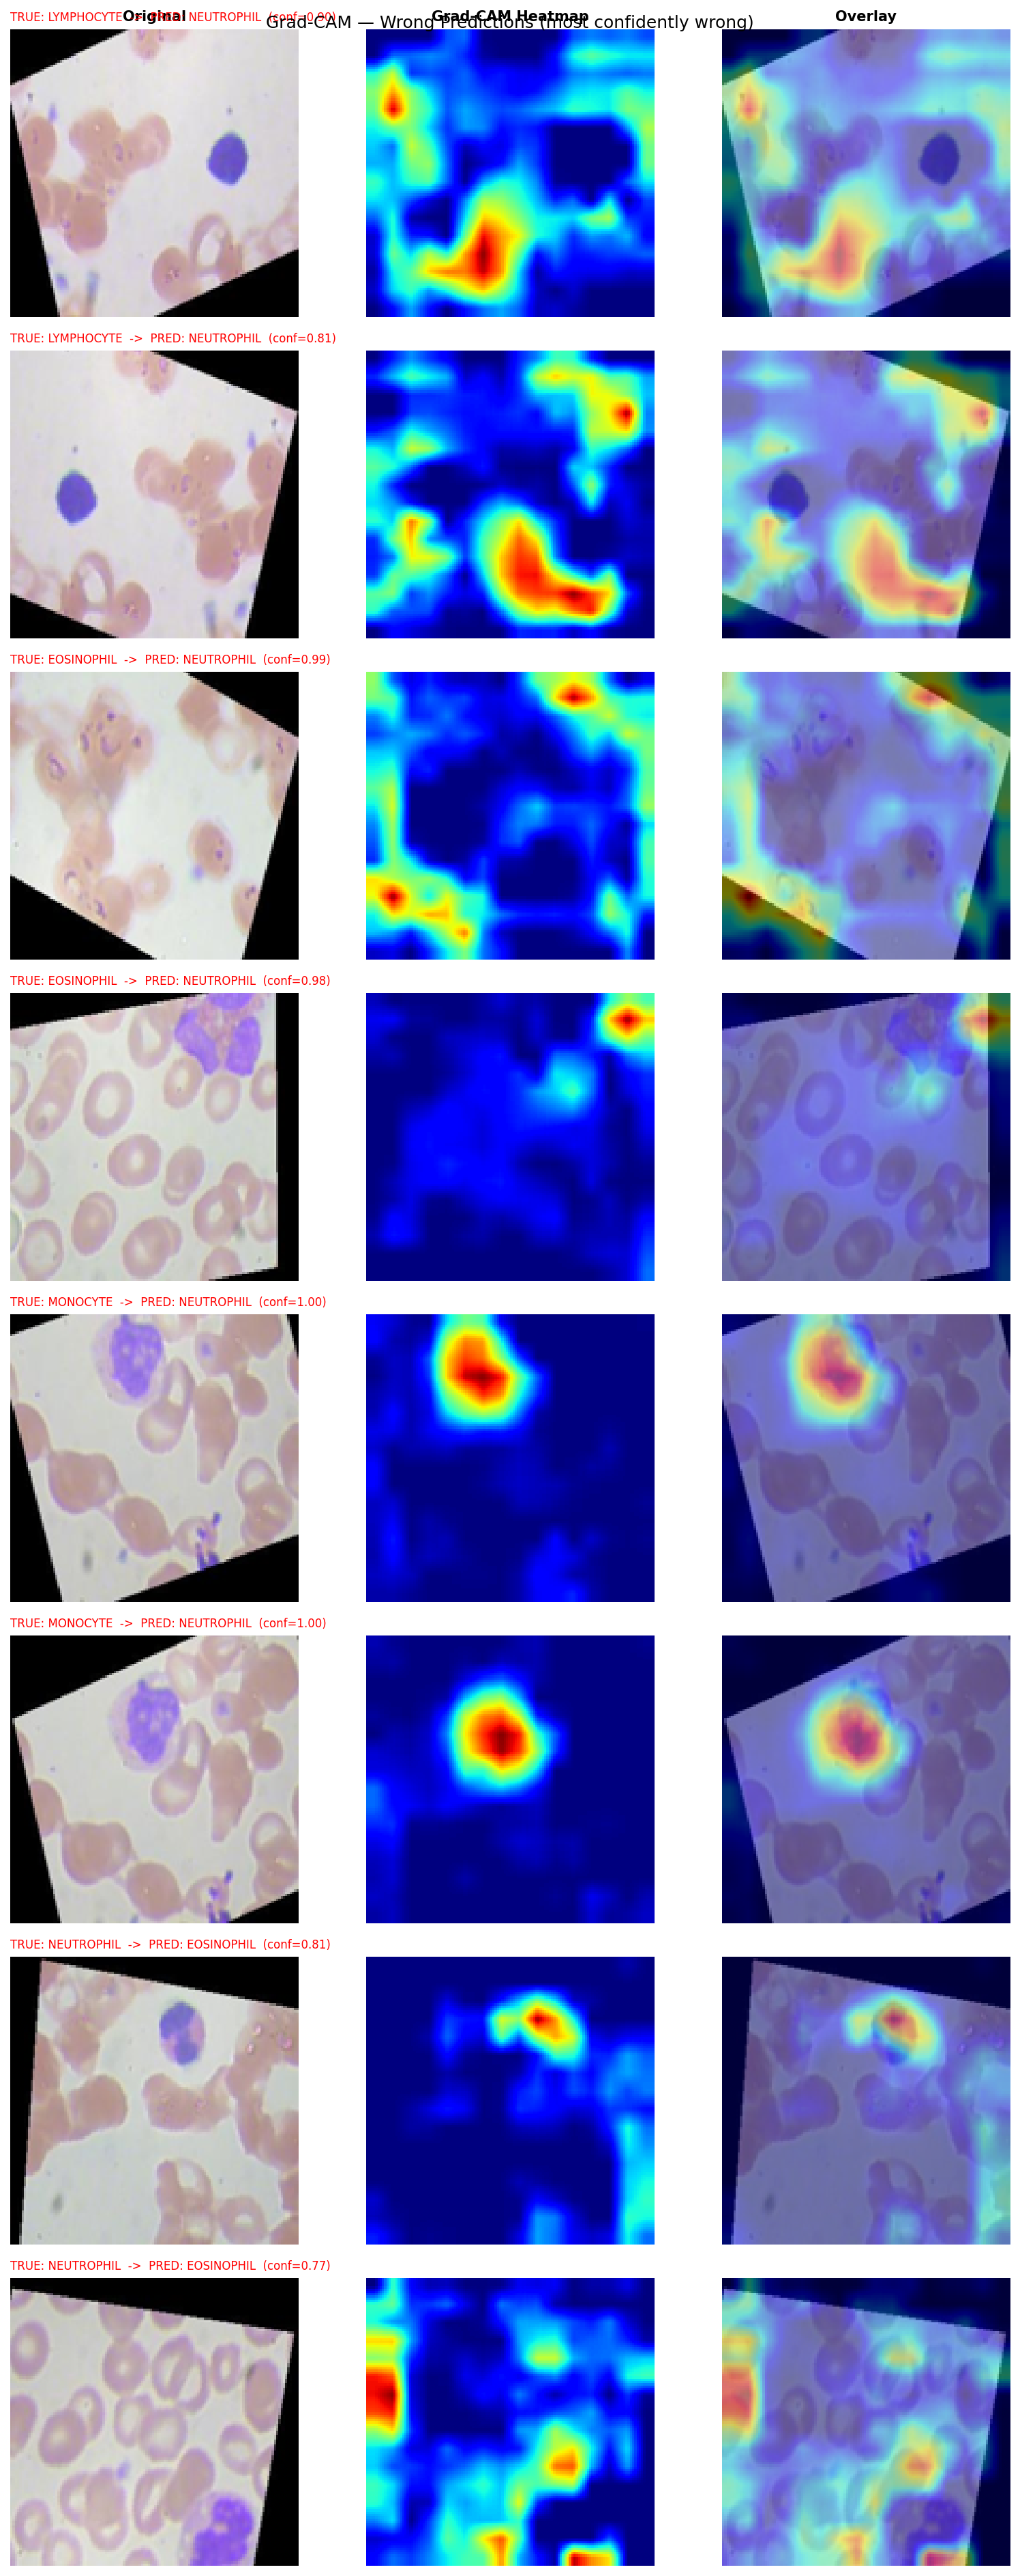
\includegraphics[width=0.45\textwidth]{../outputs/figures/phase4_04_gradcam_wrong.png}
    \caption{\lr{Grad-CAM} برای پیش‌بینی‌های اشتباه}
    \label{fig:phase4_gcam_wrong}
\end{figure}

تفاوت با نمونه‌های درست کاملاً مشهوده. نقشه‌ی حرارتی پراکنده‌ست و روی ناحیه‌ی مشخصی تمرکز نداره؛ در بعضی موارد مدل به پس‌زمینه یا سلول‌های قرمز اطراف توجه کرده نه به سلول اصلی. بخاطر همین وقتی مدل گیج می‌شه، به جای پیدا کردن ویژگی تمایزدهنده، به اطلاعات زمینه‌ای تکیه می‌کنه.

شکل~\ref{fig:phase4_gcam_cmp} این تفاوت رو برای دو کلاس به صورت مقایسه‌ای نشون می‌ده.

\begin{figure}[H]
    \centering
    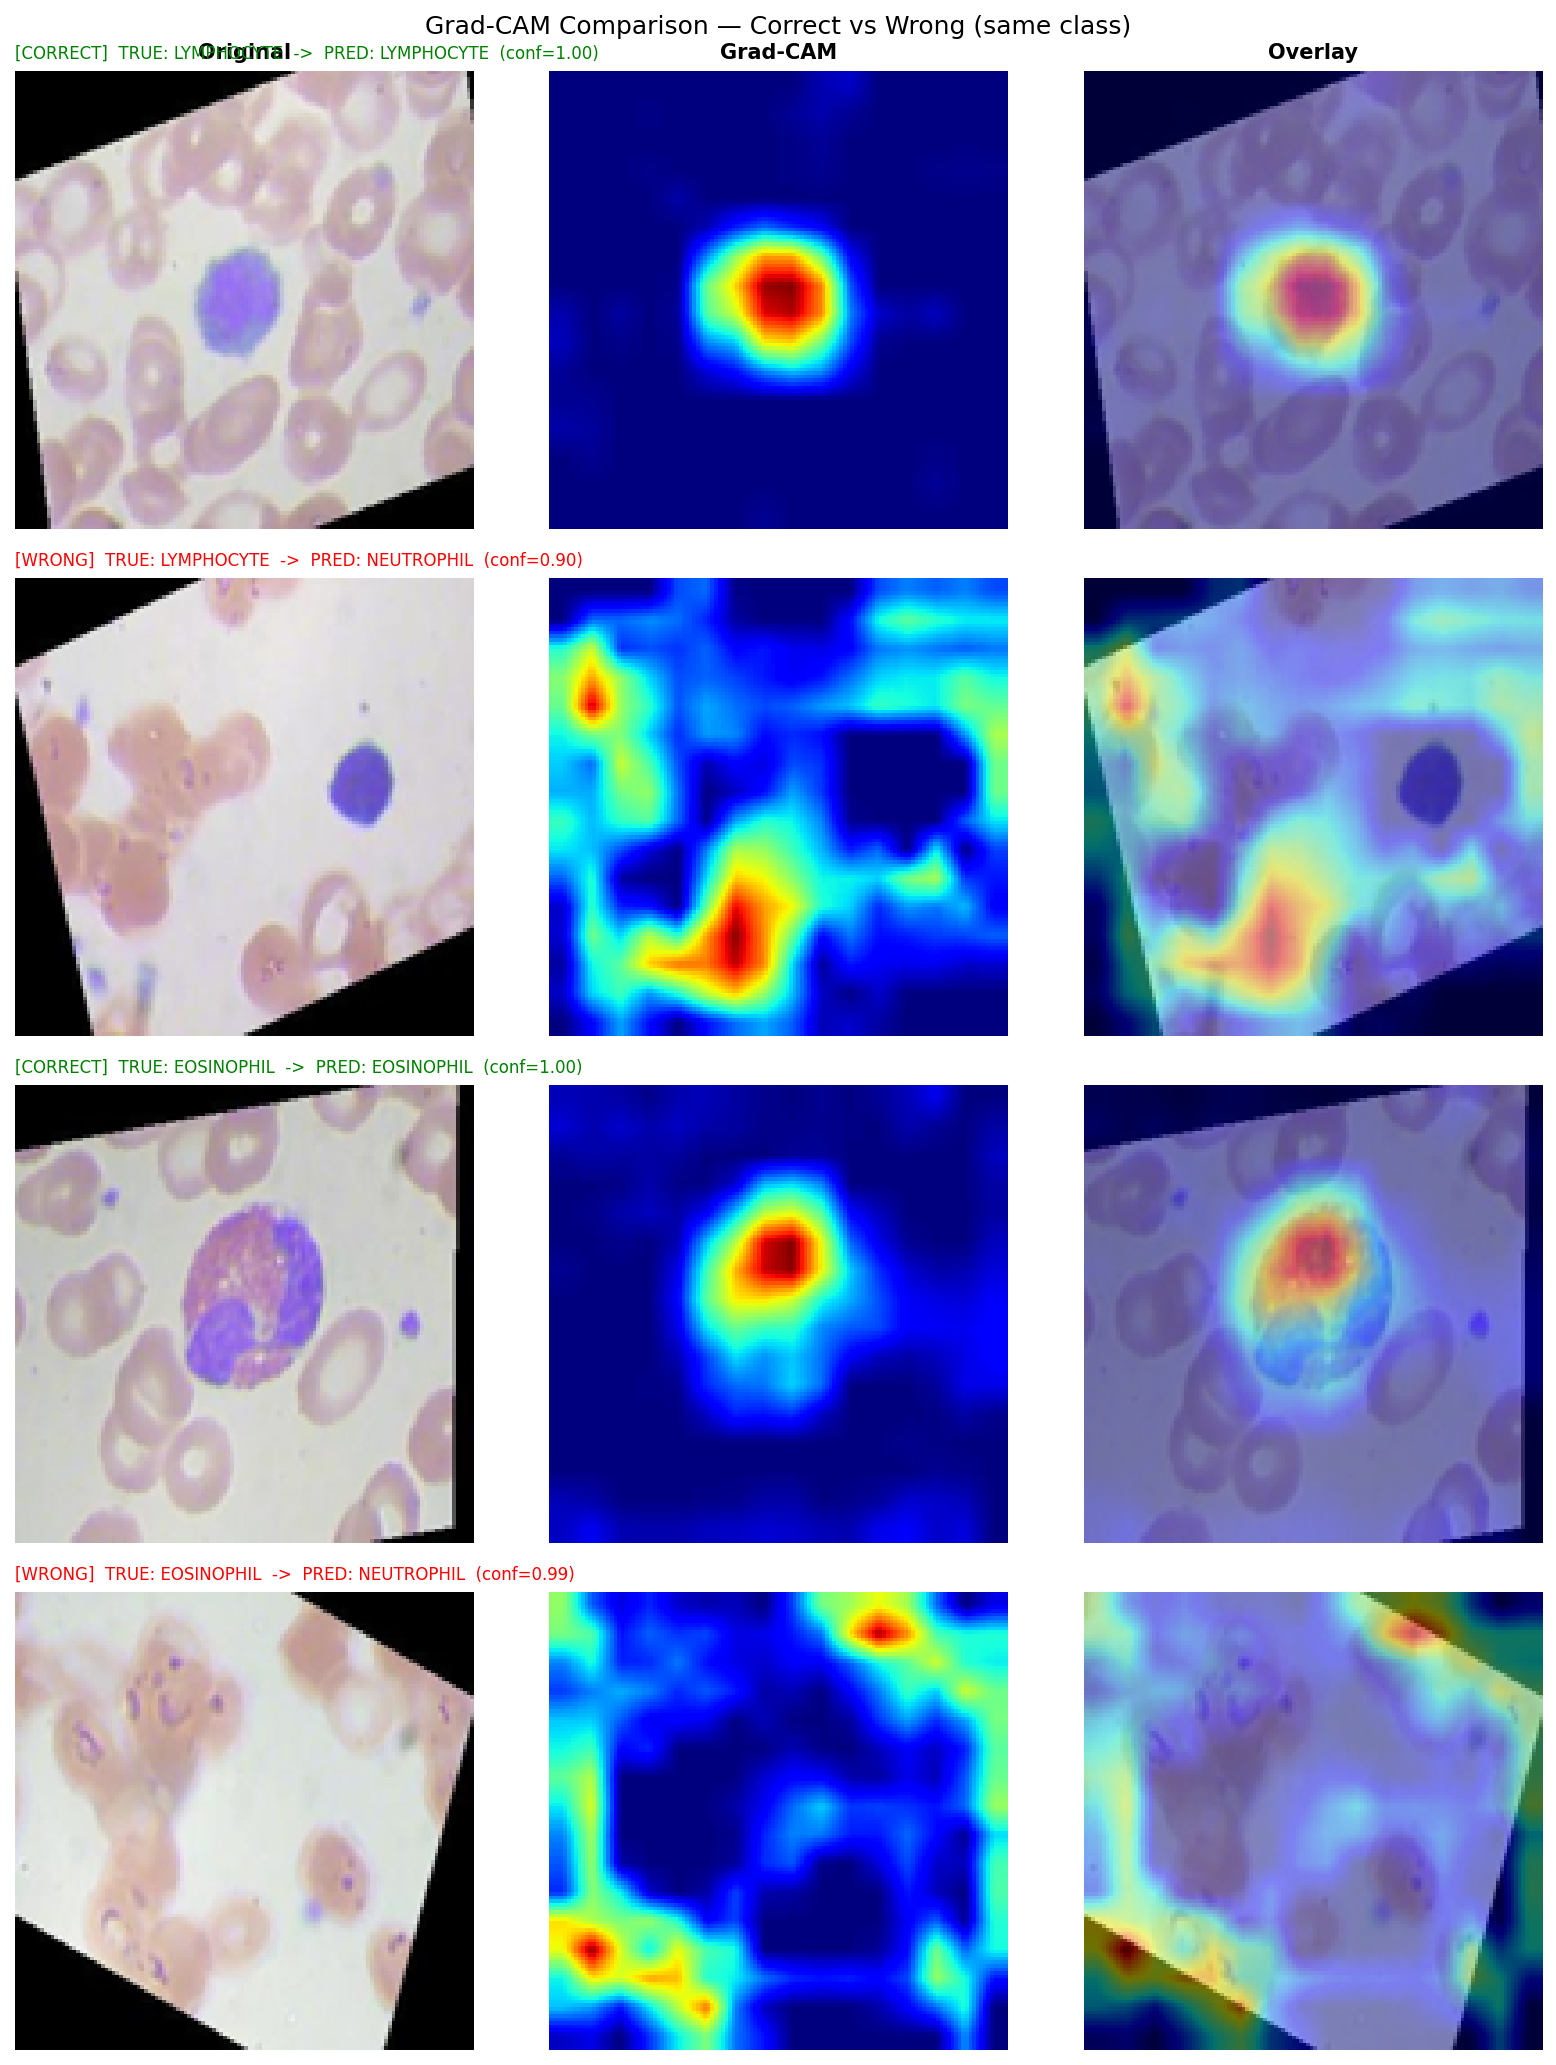
\includegraphics[width=0.72\textwidth]{../outputs/figures/phase4_05_gradcam_comparison.png}
    \caption{مقایسه‌ی \lr{Grad-CAM} برای پیش‌بینی درست و اشتباه از یک کلاس}
    \label{fig:phase4_gcam_cmp}
\end{figure}

در نمونه‌ی درست \lr{LYMPHOCYTE} نقطه‌ی داغ دقیقاً روی هسته‌ی گرد و بزرگه — همون چیزیه که این سلول رو بصری متمایز می‌کنه. در نمونه‌ی اشتباه همون کلاس که به \lr{NEUTROPHIL} تشخیص داده شده، توجه مدل پراکنده‌ست و به سلول‌های قرمز اطراف هم کشیده شده. برای \lr{EOSINOPHIL} هم همین الگو تکرار می‌شه: نمونه‌ی درست روی هسته‌ی چندلوبه‌ای متمرکزه، نمونه‌ی اشتباه روی هیچ ناحیه‌ی مشخصی تمرکز نداره. درنتیجه این تحلیل دلیل \lr{Recall} پایین \lr{LYMPHOCYTE} (\lr{0.55}) و \lr{EOSINOPHIL} (\lr{0.66}) در فاز سوم رو روشن می‌کنه: مدل در نمونه‌های دشوار نمی‌تونه ویژگی تمایزدهنده رو پیدا کنه.

% ---- 7 ----
\section{یادگیری انتقالی با \lr{MobileNetV2}}

در فازهای قبل بهترین دقت آزمون به \lr{72.38\%} رسید. یه دلیل اصلیش اینه که توزیع مجموعه‌ی \lr{TRAIN} با \lr{TEST} جابجاست — ویژگی‌هایی که مدل از داده‌های آموزشی یاد گرفته با آنچه در آزمون می‌بینه کاملاً منطبق نیست. حالا مدل‌های از‌پیش‌آموزش‌دیده روی \lr{ImageNet} این مشکل رو کاهش می‌دن، چون از همون اول ویژگی‌های پایه‌ای قوی‌تری دارن که بهتر تعمیم می‌یابن.

برای این فاز از \lr{MobileNetV2} استفاده کردیم. خوبیش اینه که نسبت به گزینه‌های سنگین‌تر مثل \lr{ResNet50} یا \lr{EfficientNet} پارامتر کمتری داره و روی \lr{GPU}های معمولی راحت‌تر آموزش می‌بینه؛ بدیش اینه که در مقابل اون مدل‌های بزرگ‌تر، سقف دقتش پایین‌تره — ولی برای این دیتاست کافیه.

\subsection{تغییر لایه‌ی خروجی}

\lr{MobileNetV2} در حالت استاندارد برای طبقه‌بندی \lr{1000} کلاس \lr{ImageNet} طراحی شده. برای تطبیق با مسئله‌ی ما که ۴ کلاسه، لایه‌ی \lr{top} اصلی حذف شد (\lr{include\_top=False}) و یه سر طبقه‌بند سبک جایگزینش شد که از سه بخش تشکیل می‌شه. اول \lr{GlobalAveragePooling2D} که خروجی سه‌بُعدی پشته‌ی کانولوشنی رو به یه بردار یک‌بُعدی تبدیل می‌کنه — در مقایسه با \lr{Flatten} پارامتر کمتری داره و به موقعیت مکانی ویژگی‌ها حساسیت کمتری نشون می‌ده. بعدش یه لایه‌ی \lr{Dropout} برای جلوگیری از \lr{overfitting} سر طبقه‌بند. و در آخر \lr{Dense(4, softmax)} که لایه‌ی خروجی با ۴ نورون برای چهار کلاس سلول خونیه.

یه نکته‌ی پیاده‌سازی مهم اینه که در \lr{forward pass}، مدل پایه با آرگومان \lr{training=False} فراخوانی می‌شه. این کار لایه‌های \lr{BatchNormalization} درون \lr{MobileNetV2} رو در حالت استنتاج نگه می‌داره — یعنی از میانگین و واریانس تجمیعی استفاده می‌کنن نه از آمار دسته‌ی جاری. بدون این تنظیم، آموزش سر طبقه‌بند با پارامترهای \lr{BN} فریز ناپایدار می‌شه.

\subsection{پیش‌پردازش ورودی}

\lr{MobileNetV2} انتظار داره پیکسل‌ها در بازه‌ی $[-1, +1]$ باشن، نه $[0, 1]$. بخاطر همین به جای تقسیم ساده بر \lr{255}، از تابع \lr{mobilenet\_v2.preprocess\_input} استفاده شد که پیکسل‌ها رو از $[0, 255]$ به $[-1, +1]$ نگاشت می‌کنه. این تفاوت ظاهراً جزئیه ولی در عمل تأثیر قابل‌توجهی روی کیفیت آموزش داره — چون وزن‌های \lr{ImageNet} با همین توزیع ورودی بهینه شدن و اگه این نگاشت رو نکنی، انگار داری با زبان اشتباه باهاشون حرف می‌زنی.

\subsection{پروتکل آموزش دو مرحله‌ای}

\subsubsection{مرحله‌ی اول — آموزش سر طبقه‌بند}

در مرحله‌ی اول تمام لایه‌های \lr{MobileNetV2} منجمد (\lr{freeze}) شدن و فقط لایه‌های سر طبقه‌بند آموزش دیدن. نرخ یادگیری $10^{-3}$ انتخاب شد — چون این لایه‌ها از صفر شروع می‌کنن و می‌شه با قدم‌های بزرگ‌تر آموزش داد. هدف اینه که سر طبقه‌بند اول یاد بگیره ویژگی‌های \lr{MobileNetV2} رو تفسیر کنه، بدون اینکه وزن‌های از‌پیش‌آموزش‌دیده رو خراب کنه.

\subsubsection{مرحله‌ی دوم — \lr{Fine-tuning} لایه‌های بالایی}

پس از همگرایی مرحله‌ی اول، چند لایه‌ی آخر \lr{backbone} از حالت منجمد خارج (\lr{unfreeze}) شدن و آموزش با نرخ یادگیری خیلی کوچیک‌تر ($10^{-5}$) ادامه یافت. دلیل انتخاب این نرخ یادگیری کوچیک اینه که وزن‌های \lr{ImageNet} در این لایه‌ها از قبل خوبن — فقط نیاز به تطبیق ظریف با دامنه‌ی تصاویر خون داریم. اگه نرخ یادگیری بالا باشه، این وزن‌ها خراب می‌شن و دقت به سطح تصادفی سقوط می‌کنه.

\subsection{تنظیم ابرپارامترها}

کلاً چهار آزمایش انجام شد — دو تا در مرحله‌ی اول با \lr{Dropout} متفاوت، دو تا در مرحله‌ی دوم با تعداد لایه‌های \lr{unfreeze} متفاوت.

\begin{table}[H]
    \centering
    \begin{tabular}{clcccc}
        \toprule
        \textbf{آزمایش} & \textbf{شرح} & \textbf{مرحله} & \textbf{\lr{Dropout}} & \textbf{لایه‌های آزادشده} & \textbf{بهترین \lr{Val Acc}} \\
        \midrule
        \lr{exp1} & سر منجمد، \lr{Dropout} سبک & \lr{1} & \lr{0.3} & ---                  & \lr{88.85\%} \\
        \lr{exp2} & سر منجمد، \lr{Dropout} قوی & \lr{1} & \lr{0.5} & ---                  & \lr{84.58\%} \\
        \lr{exp3} & \lr{Fine-tune} کم‌عمق       & \lr{2} & بهترین \lr{S1} & \lr{30} لایه‌ی آخر & \lr{98.95\%} \\
        \lr{exp4} & \lr{Fine-tune} عمیق‌تر       & \lr{2} & بهترین \lr{S1} & \lr{50} لایه‌ی آخر & \lr{99.60\%} \\
        \bottomrule
    \end{tabular}
    \caption{آزمایش‌های تنظیم ابرپارامتر — فاز پنجم}
    \label{tab:phase5_experiments}
\end{table}

در هر دو مرحله از \lr{EarlyStopping} با ویت \lr{7} و \lr{ReduceLROnPlateau} با فاکتور \lr{0.5} و ویت \lr{4} استفاده شد تا هم از آموزش بیش از حد جلوگیری بشه، هم نوسانات نرخ یادگیری کنترل بشه.

\subsection{نمودارهای آموزش}

شکل~\ref{fig:phase5_curves} نمودارهای دقت و \lr{Loss} رو برای هر چهار آزمایش نشون می‌ده.

\begin{figure}[H]
    \centering
    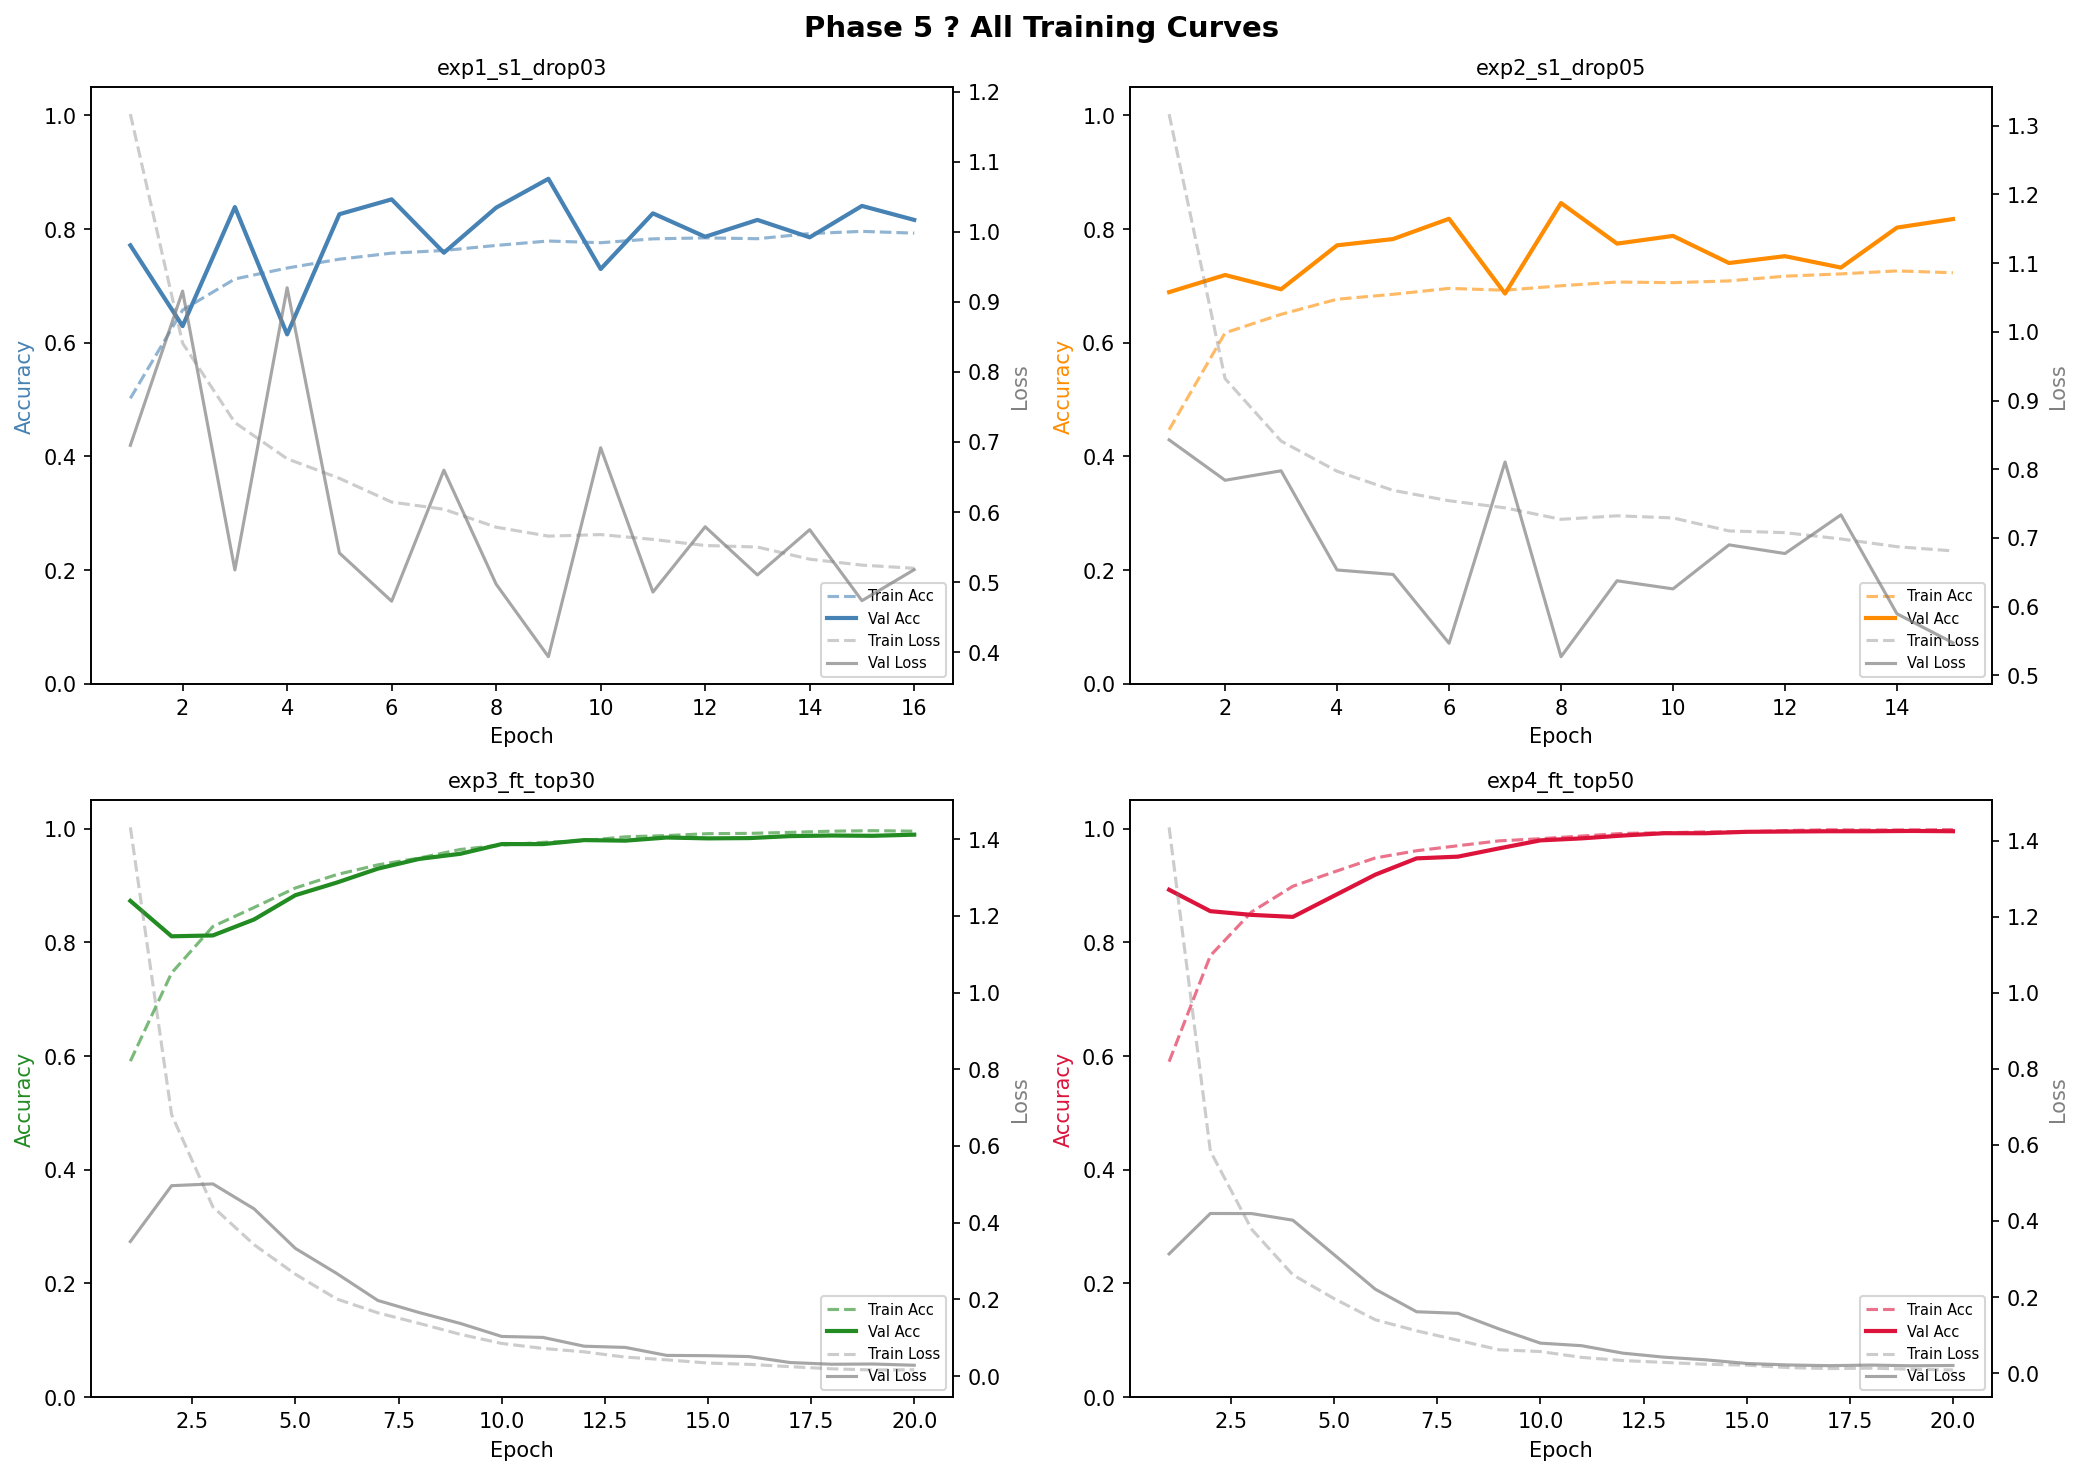
\includegraphics[width=\textwidth]{../reports/figures/phase5_01_all_curves.png}
    \caption{نمودارهای آموزش چهار آزمایش — فاز پنجم}
    \label{fig:phase5_curves}
\end{figure}

در آزمایش‌های مرحله‌ی اول (\lr{exp1} و \lr{exp2}) دقت اعتبارسنجی نسبتاً سریع به یه سقف می‌رسه، چون تمام قدرت ویژگی‌سازی از \lr{ImageNet} میاد و سر طبقه‌بند فقط باید یاد بگیره این ویژگی‌ها رو تفسیر کنه. در آزمایش‌های مرحله‌ی دوم (\lr{exp3} و \lr{exp4}) آموزش از جایی که مرحله‌ی اول متوقف شده ادامه می‌یابه و با قدم‌های آرام‌تری بهبود پیدا می‌کنه — انگار داری یه مدل نیمه‌تمام رو با دقت بیشتر تنظیم می‌کنی.

\subsection{ارزیابی روی مجموعه‌ی آزمون}

\subsubsection{ماتریس درهم‌ریختگی}

شکل~\ref{fig:phase5_cm} ماتریس درهم‌ریختگی رو برای بهترین مدل مرحله‌ی اول و بهترین مدل مرحله‌ی دوم نشون می‌ده.

\begin{figure}[H]
    \centering
    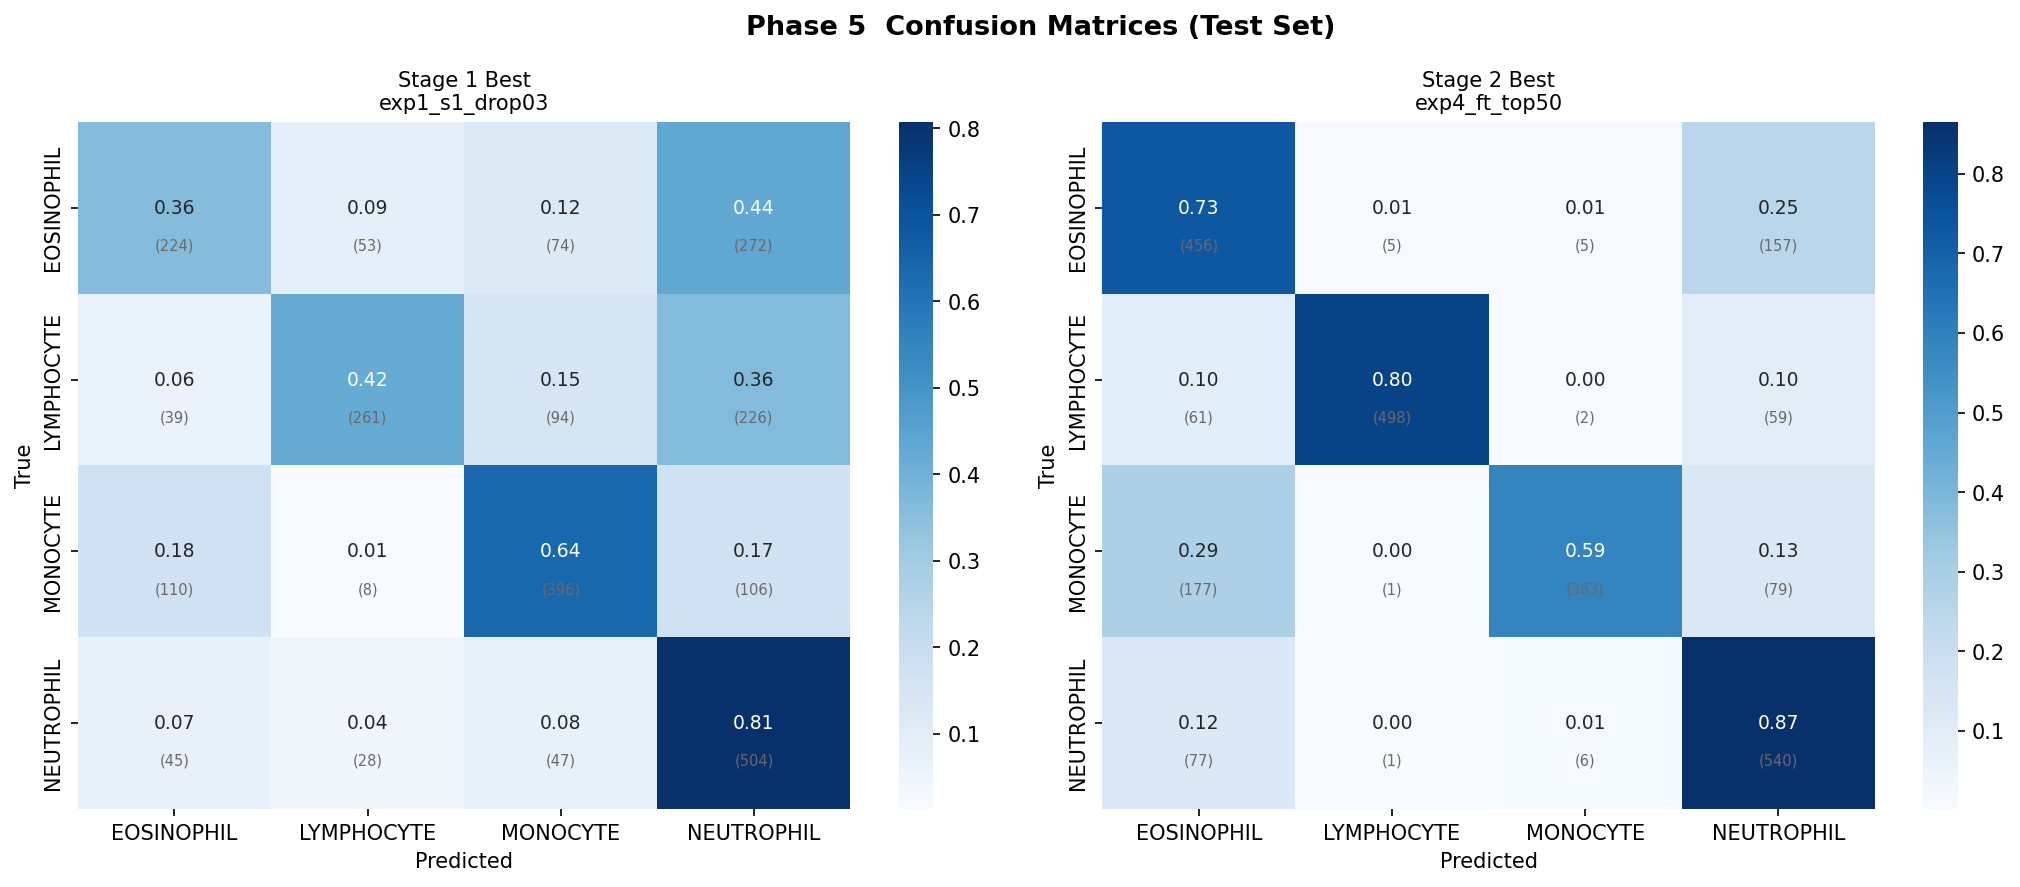
\includegraphics[width=\textwidth]{../reports/figures/phase5_02_confusion_matrix.png}
    \caption{ماتریس درهم‌ریختگی روی مجموعه‌ی آزمون — مرحله‌ی اول و دوم}
    \label{fig:phase5_cm}
\end{figure}

\subsubsection{منحنی‌های \lr{ROC}}

شکل~\ref{fig:phase5_roc} منحنی‌های \lr{ROC} رو به تفکیک کلاس نشون می‌ده. مساحت زیر منحنی (\lr{AUC}) برای هر کلاس در داخل نمودار درج شده.

\begin{figure}[H]
    \centering
    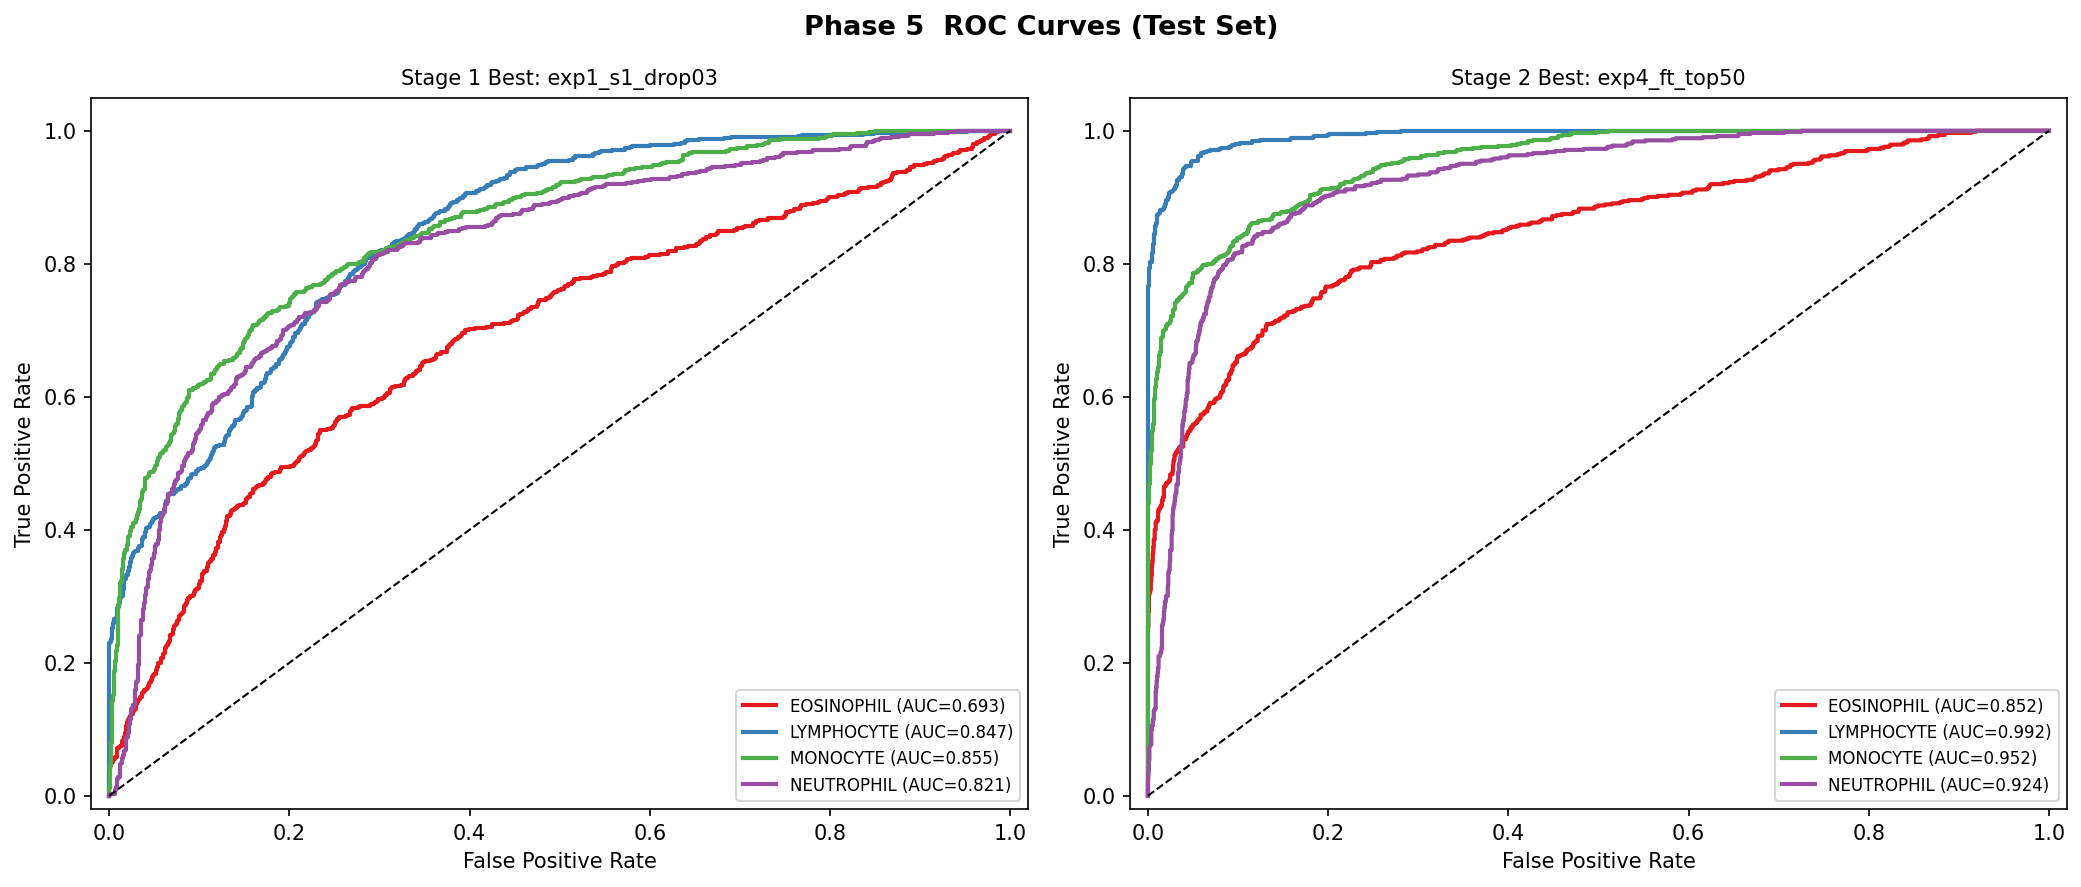
\includegraphics[width=\textwidth]{../reports/figures/phase5_03_roc_curves.png}
    \caption{منحنی‌های \lr{ROC} روی مجموعه‌ی آزمون — مرحله‌ی اول و دوم}
    \label{fig:phase5_roc}
\end{figure}

\subsubsection{نمونه‌های پیش‌بینی}

شکل~\ref{fig:phase5_samples} شانزده نمونه از مجموعه‌ی آزمون رو با برچسب واقعی و برچسب پیش‌بینی‌شده نشون می‌ده. پیش‌بینی‌های درست با کادر سبز و اشتباه‌ها با کادر قرمز مشخص شدن.

\begin{figure}[H]
    \centering
    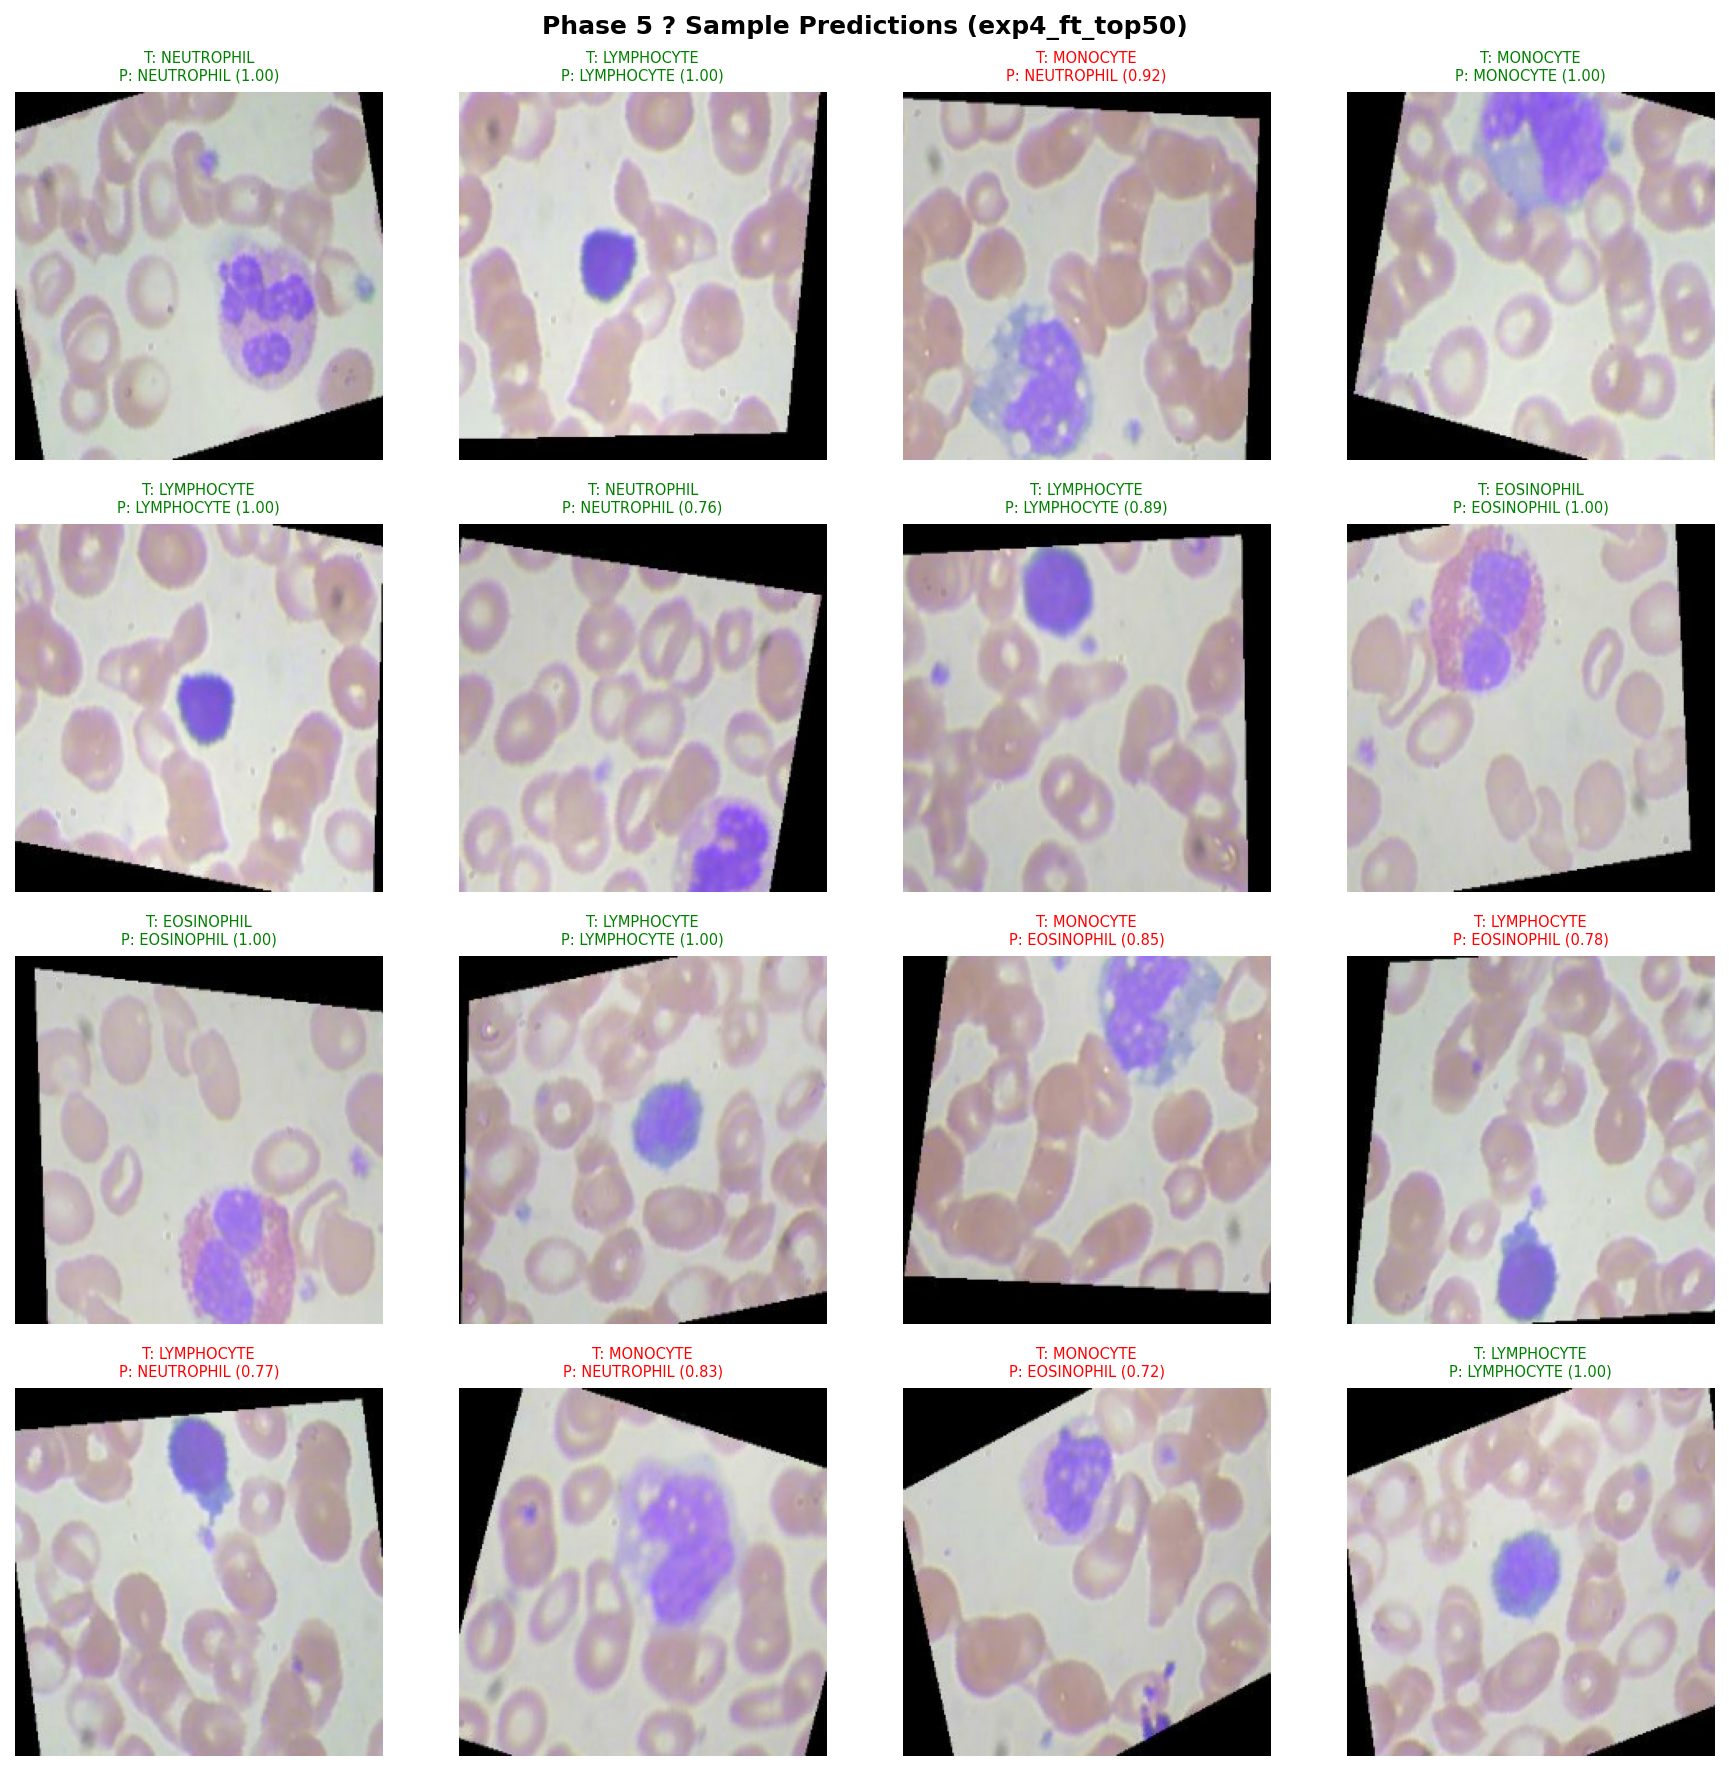
\includegraphics[width=0.9\textwidth]{../reports/figures/phase5_04_sample_predictions.png}
    \caption{نمونه‌های پیش‌بینی روی مجموعه‌ی آزمون — بهترین مدل فاز پنجم}
    \label{fig:phase5_samples}
\end{figure}

\subsubsection{معیارهای کلاس به کلاس روی مجموعه‌ی آزمون}

جدول~\ref{tab:phase5_test} نتایج دقیق‌تر رو برای بهترین مدل هر مرحله نشون می‌ده — \lr{exp1} از مرحله‌ی اول (دقت کل \lr{55.69\%}) و \lr{exp4} از مرحله‌ی دوم (دقت کل \lr{74.67\%}).

\begin{table}[H]
    \centering
    \begin{tabular}{llcccc}
        \toprule
        \textbf{مدل} & \textbf{کلاس} & \textbf{\lr{Precision}} & \textbf{\lr{Recall}} & \textbf{\lr{F1}} & \textbf{\lr{Support}} \\
        \midrule
        \multirow{5}{*}{\lr{exp4} (مرحله‌ی دوم)}
            & \lr{EOSINOPHIL} & \lr{0.59} & \lr{0.73} & \lr{0.65} & \lr{623} \\
            & \lr{LYMPHOCYTE} & \lr{0.99} & \lr{0.80} & \lr{0.89} & \lr{620} \\
            & \lr{MONOCYTE}   & \lr{0.97} & \lr{0.59} & \lr{0.73} & \lr{620} \\
            & \lr{NEUTROPHIL} & \lr{0.65} & \lr{0.87} & \lr{0.74} & \lr{624} \\
            & \lr{Macro avg}  & \lr{0.80} & \lr{0.75} & \lr{0.75} & \lr{2{,}487} \\
        \bottomrule
    \end{tabular}
    \caption{معیارهای کلاس به کلاس روی مجموعه‌ی آزمون — بهترین مدل مرحله‌ی دوم (\lr{exp4})}
    \label{tab:phase5_test}
\end{table}

\lr{Fine-tuning} عمیق‌تر (\lr{exp4}) تونست دقت کل رو از \lr{55.69\%} مرحله‌ی اول به \lr{74.67\%} برسونه — که یه جهش قابل توجهه. بهترین کلاس \lr{LYMPHOCYTE} با \lr{F1=0.89} و ضعیف‌ترین \lr{EOSINOPHIL} با \lr{F1=0.65} بود.

\subsection{مقایسه‌ی نهایی با فازهای قبل}

جدول~\ref{tab:phase_comparison} دقت آزمون تمام فازها رو کنار هم می‌ذاره و شکل~\ref{fig:phase5_cmp} همین مقایسه رو به صورت نمودار میله‌ای نشون می‌ده.

\begin{table}[H]
    \centering
    \begin{tabular}{lcc}
        \toprule
        \textbf{مدل} & \textbf{فاز} & \textbf{دقت آزمون} \\
        \midrule
        بهترین \lr{CNN} سفارشی       & فاز دوم  & \lr{69.98\%} \\
        بهترین \lr{CNN} بهبودیافته   & فاز سوم  & \lr{72.38\%} \\
        \lr{MobileNetV2} مرحله‌ی اول & فاز پنجم & \lr{55.69\%} \\
        \lr{MobileNetV2} مرحله‌ی دوم & فاز پنجم & \lr{74.67\%} \\
        \bottomrule
    \end{tabular}
    \caption{مقایسه‌ی دقت آزمون در تمام فازها}
    \label{tab:phase_comparison}
\end{table}

\begin{figure}[H]
    \centering
    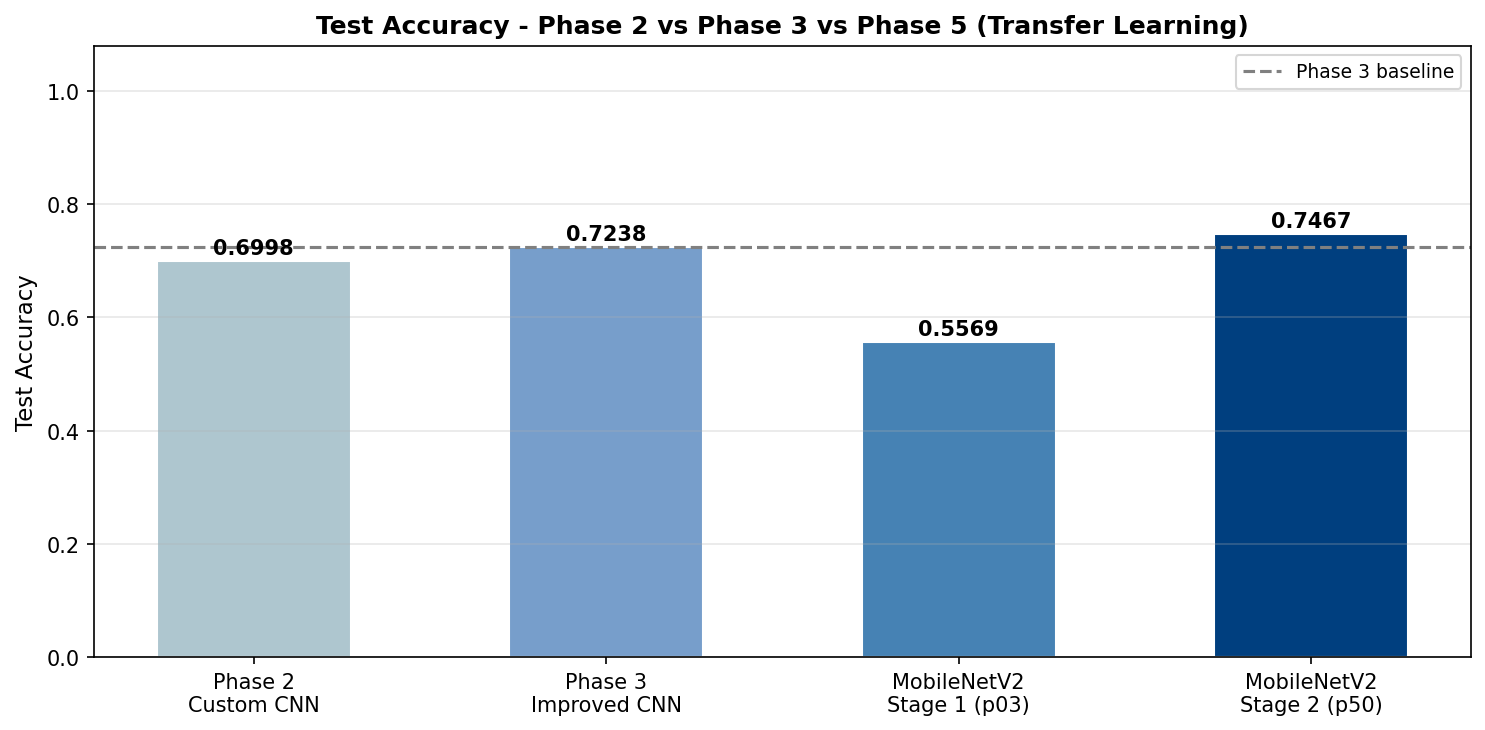
\includegraphics[width=0.85\textwidth]{../reports/figures/phase5_05_phase_comparison.png}
    \caption{مقایسه‌ی دقت آزمون — فاز دوم، سوم، و پنجم}
    \label{fig:phase5_cmp}
\end{figure}

\subsection{تحلیل نهایی}

نتایج این فاز تصویر جالب و در عین حال صادقانه‌ای از محدودیت‌های این دیتاست ارائه می‌ده.

\textbf{شکاف اعتبارسنجی و آزمون.}
بزرگ‌ترین چیزی که این فاز آشکار کرد همون مشکلیه که از فاز سوم می‌شناختیمش: جابجایی توزیع میان \lr{TRAIN} و \lr{TEST}. \lr{exp1} در اعتبارسنجی به \lr{88.85\%} رسید اما روی آزمون فقط \lr{55.69\%} داد — یعنی مدل با وجود وزن‌های \lr{ImageNet}، به همون دام \lr{overfitting} به توزیع آموزشی افتاد. \lr{exp4} این شکاف رو کوچیک‌تر کرد: اعتبارسنجی \lr{99.60\%}، آزمون \lr{74.67\%}. شکاف هنوز وجود داره، که نشون می‌ده ریشه‌ی مشکل در خود دیتاسته، نه فقط در معماری مدل.

\textbf{مقایسه با فازهای قبل.}
بهترین مدل این فاز (\lr{exp4} با دقت آزمون \lr{74.67\%}) نسبت به بهترین مدل فاز سوم (\lr{72.38\%}) حدود \lr{2.3} واحد درصد بهتر شد. این بهبود کوچیک‌تر از اون چیزیه که معمولاً از \lr{Transfer Learning} انتظار می‌ره؛ ولی با توجه به جابجایی توزیع دیتاست قابل توضیحه — وزن‌های \lr{ImageNet} کمک کردن ویژگی‌های بهتری استخراج بشه، اما مشکل اصلی که تفاوت توزیعه با هیچ معماری‌ای به‌تنهایی برطرف نمی‌شه.

\textbf{تحلیل کلاس به کلاس.}
در بهترین مدل (\lr{exp4}) کلاس \lr{LYMPHOCYTE} با \lr{Precision} بالای \lr{0.99} بهترین عملکرد رو داشت — شاید چون این سلول ویژگی بصری مشخص‌تری (هسته‌ی گرد بزرگ) داره که \lr{MobileNetV2} به خوبی یادش گرفته. در مقابل، \lr{MONOCYTE} با \lr{Recall} پایین \lr{0.59} مشکل‌دارترین کلاس بود: مدل اکثر \lr{MONOCYTE}های واقعی رو به کلاس‌های دیگه تشخیص داده، که احتمالاً به دلیل شباهت ظاهری این سلول با \lr{LYMPHOCYTE} در نمونه‌های آزمونه.

\textbf{نتیجه‌گیری کلی.}
از میان همه‌ی مدل‌های آزمایش‌شده در این پروژه، \lr{MobileNetV2} با \lr{Fine-tuning} (\lr{exp4}) بهترین دقت آزمون رو داشت. ولی بهبودش نسبت به فاز سوم اندک بود، چون مشکل اصلی این دیتاست — جابجایی توزیع بین مجموعه‌های آموزش و آزمون — یه مشکل ساختاریه که با انتخاب معماری بهتر به‌تنهایی حل نمی‌شه. پس برای حل اساسی‌تر این مشکل، روش‌هایی مثل \lr{domain adaptation} یا جمع‌آوری داده‌ی آموزشی متنوع‌تر لازمه.

\end{document}
